\documentclass[11pt,a4paper]{article}

\usepackage{fullpage}
\usepackage{hyperref}
\usepackage{graphicx}
\usepackage{grffile}
\usepackage{svg}
\usepackage{subfig}
\usepackage{listings}
\usepackage{mathtools}
\usepackage{tabulary}
\usepackage{tabularx}
\usepackage{fancyhdr}
\usepackage{adjustbox}
\usepackage{amsmath}
\usepackage{amssymb}
\pagestyle{fancy}
\fancyhf{}

\renewcommand{\headrulewidth}{0pt}
\renewcommand{\footrulewidth}{0pt}

\fancypagestyle{firstpagefooter} {
	\lfoot{\tiny{Version: 21.09.2017}}
	\cfoot{}
	\rfoot{\thepage}
	
}

\lfoot{Name: Jovan Nikolic Legi: 16-947-376}
\rfoot{\thepage}

\newenvironment{conditions*}
{\par\vspace{\abovedisplayskip}\noindent
	\tabularx{\columnwidth}{>{$}l<{$} @{${}:{}$}
		>{\raggedright\arraybackslash}X}} {\endtabularx\par\vspace{\belowdisplayskip}}

\begin{document}

\title{Advanced Systems Lab Report\\ \normalsize{Autumn Semester 2017}}
\author{Name: Jovan Nikolic\\Legi: 16-947-376}
\date{
	\vspace{4cm}
	\textbf{Grading} \\
	\vspace{0.5cm}
	\begin{tabular}{|c|c|}
		\hline  \textbf{Section} & \textbf{Points} \\
		\hline  1                &                 \\ 
		\hline  2                &                 \\ 
		\hline  3                &                 \\ 
		\hline  4                &                 \\ 
		\hline  5                &                 \\ 
		\hline  6                &                 \\ 
		\hline  7                &                 \\ 
		\hline \hline Total      &                 \\
		\hline 
	\end{tabular} 
}
\maketitle
\thispagestyle{firstpagefooter}

\newpage

\section{System Overview (75 pts)}

The middleware designed consists of 5 key units: \textbf{Net-Thread}, \textbf{internal request queue}, \textbf{pool with worker threads}, \textbf{instrumentation infrastructure}, \textbf{Shut-Down thread}. In the remaining of this section, each key unit will be described in detail. Illustration of most important processing phases in the middleware are given in figure \ref{Figure:illustration}. Flowchart of correct execution of the middleware is illustrated in figure \ref{Figure:flowchart}.

\begin{figure}[htp]
	\begin{center}
		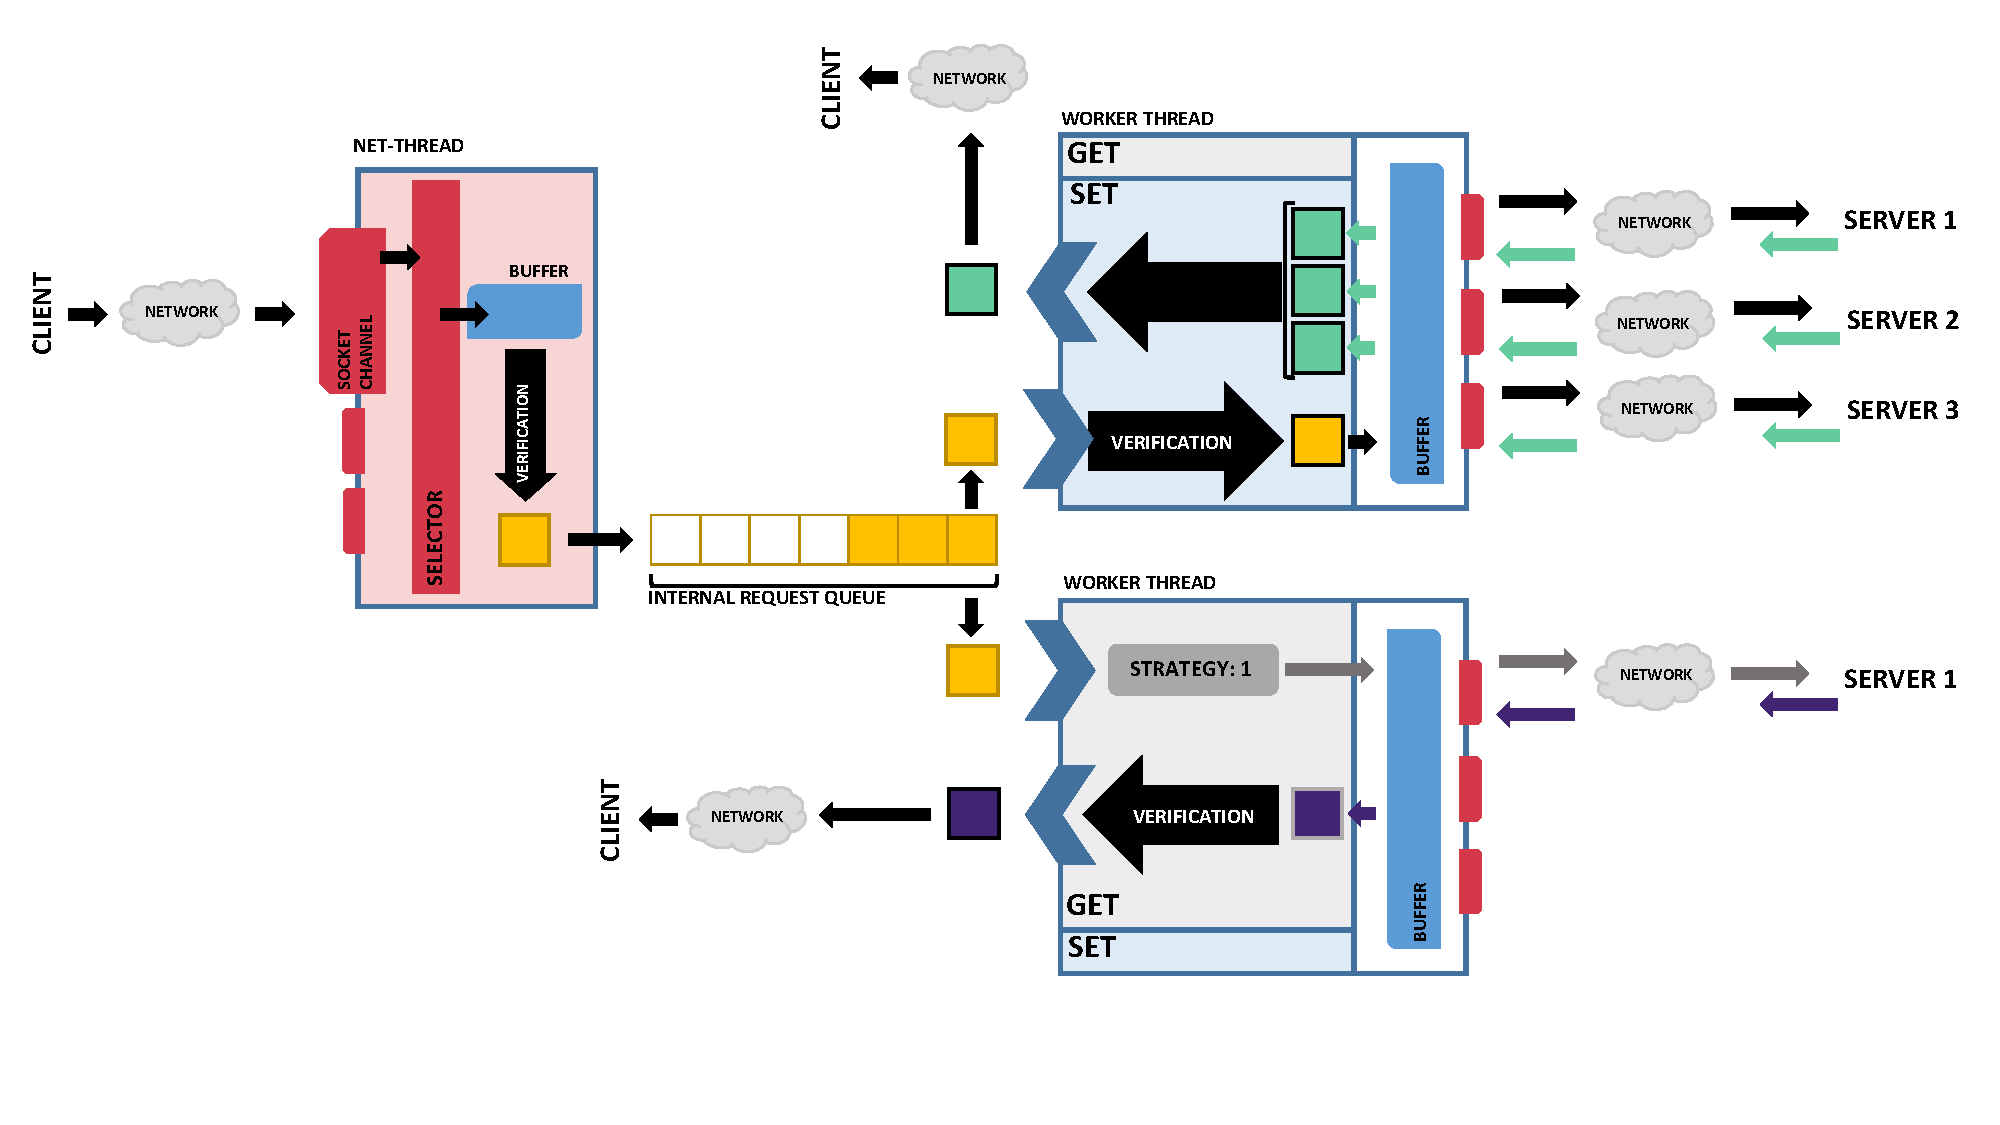
\includegraphics[width=1\linewidth]{../plots/illustration.pdf}
		\caption[illustration]{\textit{Illustration of main units and mechanisms in the middleware}. Request travels from client to the input stream of Socket Channel, Selector detects that the request has arrived, and Net-Thread reads it into the buffer and performs light verification before enqueuing it. Worker threads can support both types of requests, and here are displayed only 2 workers, each with emphasis on different type of requests. Each worker thread has its own individual buffer. For GET request, worker chooses one of the servers (here server 1) to forward the request to and then waits for a response from it. For SET requests, it forwards the request to all 3 servers, and reads responses from all of them. In both cases, worker chooses one final response and sends it back to the client (through the same individual buffer, but this is not shown here).  }
		\label{Figure:illustration}
	\end{center}
\end{figure}

\begin{figure}[htp]
	\begin{center}
		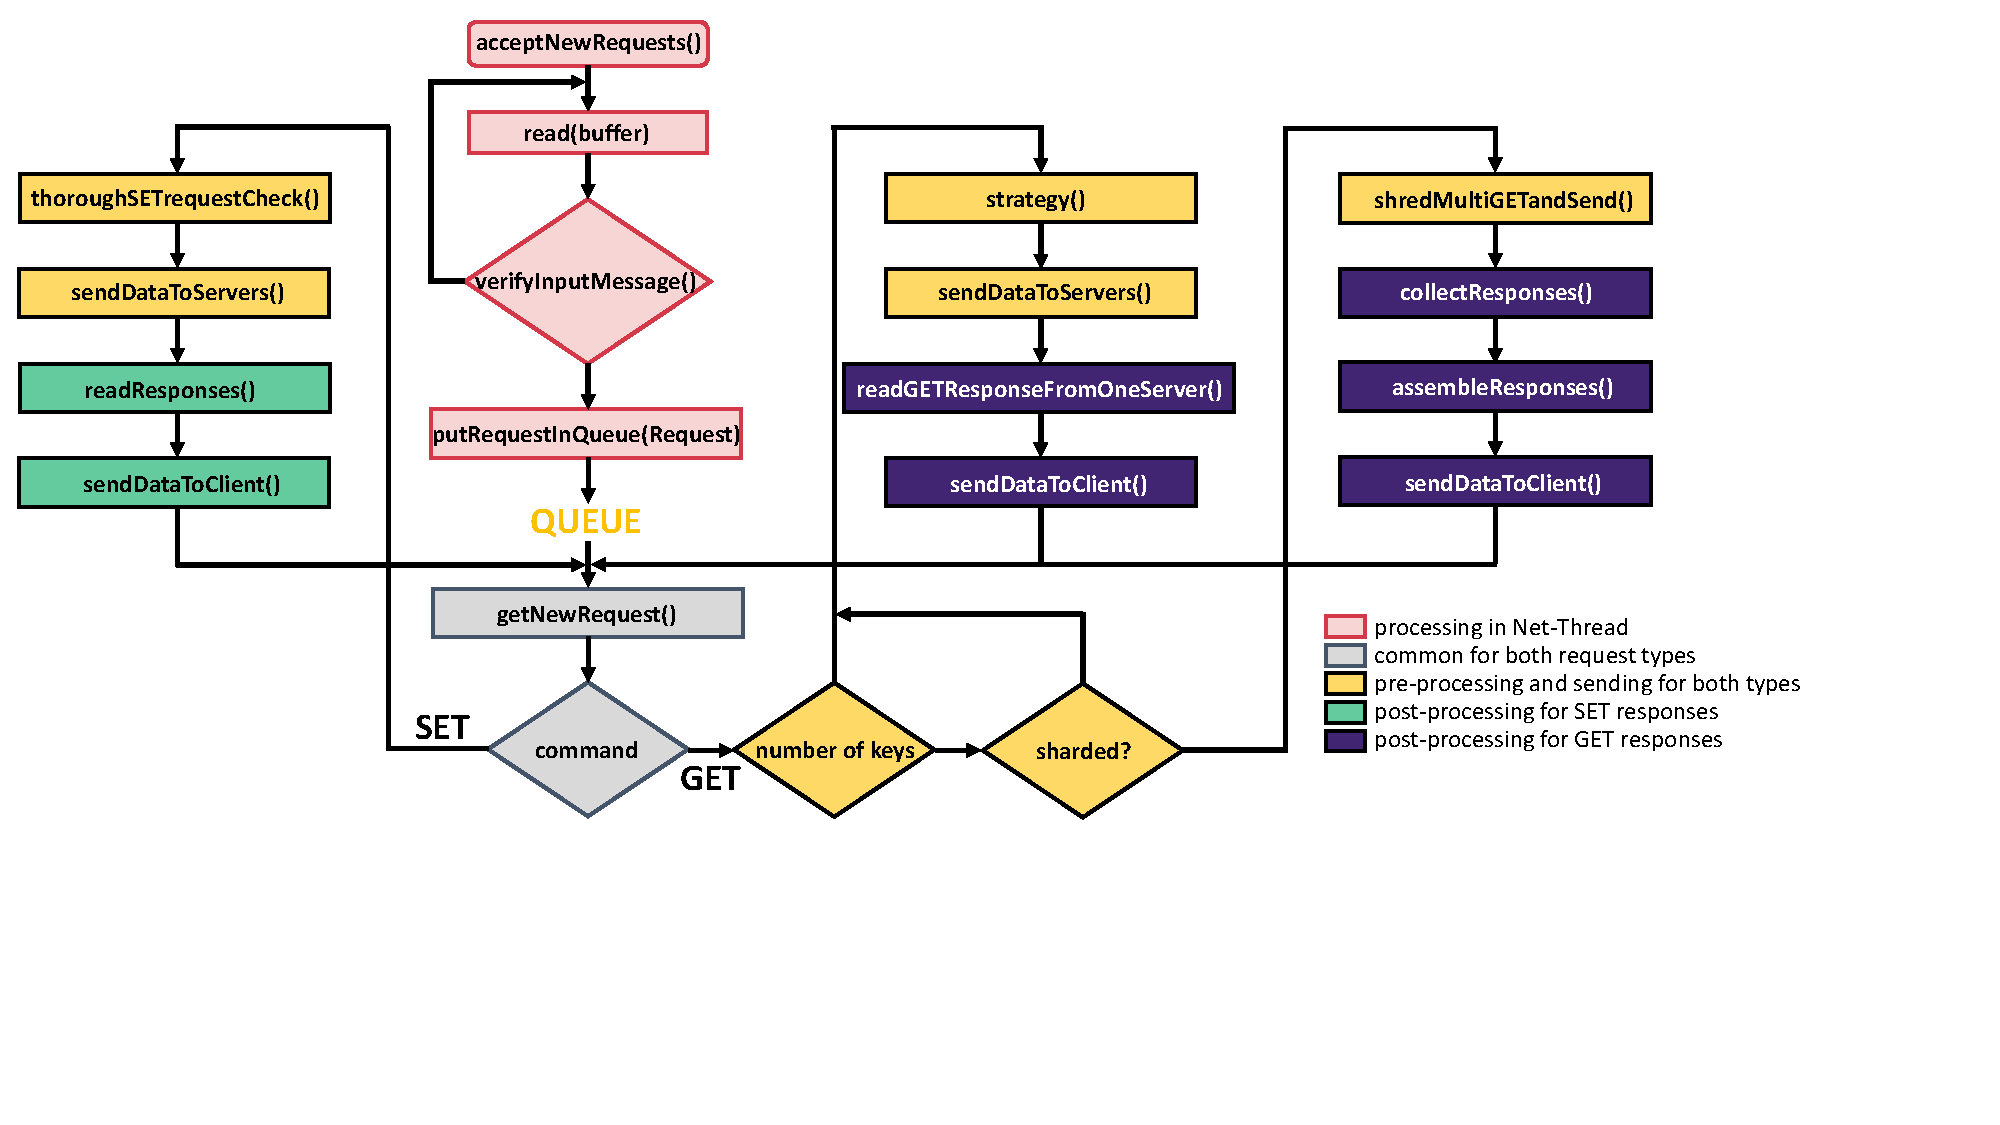
\includegraphics[width=1\linewidth]{../plots/flowchart.pdf}
		\caption[illustration]{\textit{Flowchart of method calls for correct middleware execution}.  }
		\label{Figure:flowchart}
	\end{center}
\end{figure}

\subsection{Net-Thread}

Net-Thread is the thread that receives requests from clients, performs first light processing of the requests, and stores them in the internal request queue. Net-Thread's implementation relies on \texttt{java.nio} package, specifically on \texttt{Selector}\footnote{https://docs.oracle.com/javase/8/docs/api/java/nio/channels/Selector.html}, \texttt{ServerSocketChannel}\footnote{https://docs.oracle.com/javase/8/docs/api/java/nio/channels/ServerSocketChannel.html}, \texttt{SocketChannel}\footnote{https://docs.oracle.com/javase/8/docs/api/java/nio/channels/SocketChannel.html} and \texttt{ByteBuffer}\footnote{https://docs.oracle.com/javase/8/docs/api/java/nio/ByteBuffer.html} classes. Handling multiple registered \texttt{SocketChannels} and \texttt{ServerSocketChannels} within a single thread is achieved by blocking the thread on \texttt{Selector} object, while \texttt{Channel}s remain in a non-blocking mode. \texttt{Channel}-s send and receive messages in streams. In order for message to be sent, it must first be written into a \texttt{ByteBuffer} object and then actual sending is done by \texttt{Channel}, and to receive message means to read bytes from the \texttt{Channel}'s stream into \texttt{ByteBuffer} object (\texttt{SocketChannel::read(buffer)} method in Figure \ref{Figure:flowchart}).

During Net-Thread initialization, \texttt{Selector} and \texttt{ServerSocketChannel} objects are created, and \texttt{ServerSocketChannel} is registered at \texttt{Selector}. Once \texttt{Selector} detects that new client wants to connect, Net-Thread establishes connection with the client by creating \texttt{SocketChannel} object, setting it a non-blocking mode and registering at \texttt{Selector} object as well.

With every new client accepted, a \texttt{ByteBuffer} object is created and assigned, one per new client. The buffer is then later reused for any incoming (and only incoming) traffic from the client to Net-Thread. Based on maximal sizes of SET and GET requests that middleware should handle, the capacity of \texttt{ByteBuffer} in Net-Thread (only!) is set to 2575 bytes which corresponds to multi-GET request with 10 keys, each key of maximal length of 256 bytes. 

Once new request from already accepted clients is detected (\texttt{Net-Thread:: accept New Requests()}) and received (into \texttt{ByteBuffer}), the request undergoes light verification (\texttt{Utils:: verify Input Message()} in Figure \ref{Figure:flowchart}). If the verification was successful, the message together with pointer to clients \texttt{SocketChannel} is wrapped in \texttt{Request} object and stored in internal request queue (\texttt{NetThread:: putRequestInQueue(Request)} in Figure \ref{Figure:flowchart}), and the buffer is cleared.

\textit{\textbf{Verification of requests by Net-Thread.}} The goal of the verification process is to determine if received data represents complete request:
\begin{itemize}
	\item GET request is considered fully received if it ends with bytes corresponding to \texttt{\textbackslash r\textbackslash n} and first 3 bytes correspond to "\texttt{get}".
	\item SET request is considered fully received if it ends with bytes corresponding to \texttt{\textbackslash r\textbackslash n}, first 3 bytes correspond to "\texttt{set}" and there is at least one more occurrence of bytes corresponding to \texttt{\textbackslash r\textbackslash n} between \texttt{set} and \texttt{\textbackslash r\textbackslash n} in the end.
\end{itemize}
In any other case, received data is considered incomplete. While verification of GET requests cannot produce false positives (unless keys do not conform to the protocol, e.g. keys should not contain bytes corresponding to \texttt{\textbackslash r\textbackslash n}), verification of SET requests can produce false positives. This happens in case that final bytes corresponding to \texttt{\textbackslash r\textbackslash n} do not represent end of data-block line, but are valid parts of data-block. The verification process cannot produce false negatives.

In case that verification of received data was unsuccessful, read data is kept in the buffer. When new message from the same client is detected, it is just being appended to the content of the buffer, as it is assumed that it is remaining of the message (clients cannot generate new request before receiving response from the previous request). All aforementioned actions are applied to this "appended" request as well. 

\subsection{Internal request queue}

Internal request queue is a \texttt{LinkedBlockingQueue}\footnote{https://docs.oracle.com/javase/8/docs/api/java/util/concurrent/LinkedBlockingQueue.html} object from \texttt{java.util.concurrent} package. Net-Thread enqueues \texttt{Request} objects into this queue and worker threads are removing requests from it. It is thread-safe, orders element is FCFS (First-Come-First-Served) fashion and inserting elements is successful only if adding new element would not exceed it's capacity and is a non-blocking function. On the other hand, removing elements from the queue is blocking and worker threads are blocked until queue is non-empty. Capacity of the queue is not specified, hence it is set to \texttt{Integer.MAX\char`_VALUE} which equals to $2^{31} - 1$ elements, which is more than enough. Note that this high capacity does not have extra costs in memory, since \texttt{LinkedBlockingQueue} is based on linked nodes, which are added dynamically.

\subsection{Pool of worker threads}

Class \texttt{Worker} extends \texttt{Thread}\footnote{https://docs.oracle.com/javase/8/docs/api/java/lang/Thread.html} class from \texttt{java.lang} package and represents worker thread of the middleware. Worker threads are created and started during creation of the middleware, and only then. Pointers to worker threads are stored in an \texttt{ArrayList} object, which can be considered as "worker thread pool". Number of worker threads in the "pool" is determined by command line argument. Minimal number of worker threads necessary for correct execution of the middleware is 1.

In the remaining of this section, each of specific \texttt{Worker} functionalities will be described in detail. However, instrumentation infrastructure is omitted from this list, and will be described in a separate subsection.

\subsubsection{Main Loop of the \texttt{Worker}}

After being started, all worker threads are initially blocked on the internal request queue, waiting for an element to appear in it. Once they are unblocked and request is obtained (\texttt{Worker::getNewRequest()} in Figure \ref{Figure:flowchart}), based on the type of the request, it is pre-processed accordingly and corresponding request(s) are sent to the server(s). After responses are collected, they are post-processed again according to their types, and one final response is sent to the client. Then, \texttt{Worker} gets blocked on the queue again, and so on. This loop is illustrated in Figure \ref{Figure:flowchart}.

\subsubsection{Initialization and opening and closing connections}

Initialization of \texttt{Worker} object consists of: initializing instrumentation infrastructure (described later), initializing a \texttt{ByteBuffer} object and opening connections to the servers.

Much like Net-Thread has one reusable buffer object per client, each \texttt{Worker} has one reusable \texttt{ByteBuffer} object which is used for any outgoing and incoming traffic from server(s) and for outgoing traffic towards clients. Capacity of this buffer is set according to the maximal size of the message that it should be able to handle - 13010 bytes, which corresponds to the response from multi-GET request with 10 keys where length of one key equals to 256 bytes, which is maximal key length allowed by memcached protocol, and data-block size is fixed to 1024 bytes. Allocating memory for \texttt{ByteBuffer} is an expensive operation, and often reserves more memory than necessary, which is why it is done only in the beginning. This may, however, require temporal storing of the content of the buffer in other structures (\texttt{BufferStruct}), but the content is often significantly shorter than buffer's capacity. 

\textbf{Opening connections} to servers is performed only during initialization of \texttt{Worker} object, and connections are kept open throughout whole runtime of the middleware. Unlike Net-thread, \texttt{Worker} thread does not rely on \texttt{Selector}, but only on \texttt{SocketChannel}s. There is one \texttt{SocketChannel} per server per worker thread which are all configured in a blocking mode. This means that a worker thread is blocked directly on the \texttt{SocketChannel} object until there are bytes to be read from its input stream.

\textbf{Closing connections} with servers is triggered by Shut-Down thread. Until this moment, connections to the servers are kept open.

During opening and closing of connections with servers, various exceptions can occur, which are caught and logged. However, the middleware assumes stable internet connection with servers and clients and that servers will not close connections with workers during middleware runtime. Hence, workers are not equipped with functionalities to reconnect to the servers or to overcome these exceptions anyhow.

\subsubsection{Request Pre-Processing}

In Figure \ref{Figure:flowchart}, method-calls corresponding to pre-processing phase are in yellow.

Once \texttt{Request} is obtained, it undergoes verification and pre-processing based on its type:
\begin{itemize}
	\item \textbf{SET request}: As verification in Net-thread can produce false positives, more thorough check (\texttt{Utils::thoroughSETrequestCheck()}) is performed here - the whole message is split into its (space-separated) constituents ("tokens"). Verification is successful if all the following requirements are met:
	\begin{itemize}
		\item \textit{first line}: command name equals to \texttt{set}, and there exist tokens for key, flag, expiration time and data-block size. Length of the key is not checked, and it is assumed that key is no longer than 256 bytes.
		\item \textit{second line}: length of this line (excluding final two bytes corresponding to \texttt{\textbackslash r\textbackslash n}) is equal to the number indicated in data-block size token.
	\end{itemize}
	Otherwise, the verification fails and error message is sent back to the client. Request that passed the verification successfully is then sent to all available servers (\texttt{Worker::sendData ToServers()}) in the same order in which servers were listed in command-line argument.
	\item \textbf{GET request}: Check that Net-Thread performs if received request is complete in case of GET requests cannot produce false negatives, so here further actions are determined based on number of keys in the request:
	\begin{itemize}
		\item \textbf{single GET request}: Since there is only one key, the whole received request is forwarded to the server without any additional check. Server is chosen based on a \textit{ round-robin strategy} (\texttt{Worker::strategy()}).
		\item \textbf{mutli-GET in non-sharded case}: This case is treated in the exactly same way as single GET request is. There are between 2 and 10 keys in the request.
		\item \textbf{multi-GET in sharded case}: In this case, there are between 2 and 10 keys in the request as well. The keys are equally split (\texttt{Worker::shredMultiGETandSend()}) between all servers, and matching between splits and servers is determined by the \textit{strategy}. The splittings for some special cases are given in Table \ref{(Table:sharding_example)}. Individual \texttt{get} requests are created for each of the servers and sent out.
	\end{itemize}
	
	Initially, servers are listed in the same order in which they were positioned in command-line argument. \textit{Strategy} returns next server in the list relative to the last returned server, and starts from the beginning when previous server was last in the list (round-robin). In sharded case, \textit{strategy} is invoked 2 or 3 times, thus making permutation of available servers.
	
\end{itemize}
If verification in case of SET request failed, or if GET request has 0 keys, error message is immediately sent back to the client, without forwarding the request to servers. In both cases, the same error message is sent - \texttt{ERROR\textbackslash r\textbackslash n}.

\begin{center}
	\begin{table}[!ht]
		\centering
		\begin{tabulary}{\linewidth}{ | C | C | C | C | C |}
			\hline \textbf{Number of keys}	& \textbf{Number of servers}	& \textbf{Chosen Server 1}	& \textbf{Chosen Server 2}	& \textbf{Chosen Server 3} \\ 
			\hline 2	& 2	& 1	& 1	& -	\\ 
			\hline 2	& 3	& 1	& 1	& - \\ 
			\hline 3    & 3	& 1	& 1	& 1 \\
			\hline 4	& 3	& 2	& 1	& 1	\\
			\hline 5	& 3	& 2	& 2	& 1 \\
			\hline
		\end{tabulary}
		\caption{\textit{Splitting keys between available servers in sharded case}. Identification of the servers here refer to their position in the permutation generated by \textit{round-robin strategy}.}
		\label{(Table:sharding_example)}
	\end{table}
\end{center}

\subsubsection{Request Post-Processing}

After forwarding requests to the servers, \texttt{Worker} threads are blocked on \texttt{SocketChannel}s, waiting for response from them. Based on the type of the request forwarded, different actions are taken:
\begin{itemize}
	\item \textbf{SET request}: The worker reads responses from the servers sequentially in the same order in which it had previously sent requests to them (\texttt{Worker::readResponses()} in Figure \ref{Figure:flowchart}). Once all responses are collected, \texttt{Worker} thread checks responses. If all responses are equal to the string \texttt{STORED\textbackslash r\textbackslash n}, then one of them is sent back (\texttt{Worker::SendDataToClient()} in Figure \ref{Figure:flowchart}) to the client (via reusable buffer of the worker). If any of them is not equal to this string, it is assumed that error message is received, and first error message seen by the worker is sent to the client.
	\item \textbf{single GET request}: Note that in this case, request was sent to only one server, so the worker just reads response from it (\texttt{Worker::readGETResponseFromOneServer()} in Figure \ref{Figure:flowchart}). Then, the response is verified for completeness - if final 5 bytes correspond to \texttt{END\textbackslash r\textbackslash n}, message is assumed complete. If the verification is successful, the response is just sent to the client. Otherwise, error message is sent.	
	\item \textbf{multi-GET responses in non-sharded case}: This response is treated exactly the same way as single GET request, and the same verification rules apply.
	\item \textbf{multi-GET responses in sharded case}: \texttt{Worker} thread reads responses from the servers (\texttt{Worker::collectResponses()} in Figure \ref{Figure:flowchart}) in the same order in which sharded requests were sent. Then, all individual responses undergo aforementioned verification of GET responses. Finally, responses are merged into one (\texttt{Worker::assembleResponses()} in Figure \ref{Figure:flowchart}). Given that every response contains the key and that thread receives responses from the servers in the same order it used for sending requests to them, no reordering of the responses is necessary. This merged response is then sent to the client.
\end{itemize} 

\subsection{Instrumentation infrastructure}

Instrumentation of the middleware is based on \texttt{Logger}\footnote{https://docs.oracle.com/javase/8/docs/api/java/util/logging/Logger.html} class from \texttt{java.utils.logging} package. Each \texttt{Worker} thread has its individual logging infrastructure - each worker creates and maintains its \texttt{Logger} objects and writes logs to separate files. This way there are no performance costs in synchronizing all the workers, which would exist if the \texttt{Logger} objects were shared between workers. The log files from different workers are later merged by \texttt{Python} scripts.

Each logger has a buffer with storage capacity of 20000 log messages. \texttt{Worker} threads individually force flushing in the loggers when this limit is reached.

There are 3 types of loggers in the middleware (each implemented as separate instance of \texttt{Logger} object):
\begin{itemize}
	\item \textbf{execution logger} 
	\item \textbf{logger for timings}
	\item \textbf{logger for request and load counters}
\end{itemize}  

\subsubsection{Execution Logger}

Execution logger is a global \texttt{Logger} object accessed by all classes. It contains logs of all caught exceptions, as well as crucial (correct) messages of middleware execution, such as notifications that connections between middleware and clients and servers are opened or closed. Since middleware is not supposed to have any exceptions and not many execution logs in general, logs from this logger are flushed only once by custom Shut-Down thread of the middleware. Execution logger flushes its data into \texttt{debug.log} file, where each entry includes date and time and method that is logging.

\subsubsection{Logger for timings and queue size}

Logger for timings logs \textbf{timestamps} for several key time-points in the lifecycle of \textbf{every} request in the middleware - one entry in the buffer of this logger corresponds to one processed request. Therefore, flushing of this logger is forced after every 20000\textsuperscript{th} request. This logger is individual for each worker thread.

The timestamps are the following:
\begin{enumerate}
	\item \textit{timestamp at which the request was received} by Net-Thread. It records the time Net-Thread detected (full) request in \texttt{SocketChannel} stream. If request was received in several packets, this is the time when all of them are received and detected by Net-Thread.
	\item \textit{timestamp at which the request was put in the internal request queue} by Net-Thread. This and previous timestamp are recorded by Net-Thread and then stored in \texttt{Request} object thus transferring timestamps to \texttt{Worker} thread that will actually log them.
	\item \textit{timestamp at which the request was removed from the internal request queue} by \texttt{Worker} thread.
	\item \textit{timestamp at which request(s) are sent to server(s)} by \texttt{Worker} thread. It is recorded immediately \textit{before} the first request is sent.
	\item \textit{timestamp at which complete response from server(s) is received} by \texttt{Worker} thread. It is recorded immediately \textit{after} reading last response.
	\item \textit{timestamp at which final response is sent to the client} by \texttt{Worker} thread.
\end{enumerate}
Using these timestamps, it can be measured how much time each request spends in each of the processing phases in the middleware. The most important are:
\begin{itemize}
	\item \textit{\textbf{response time}} of one request is the difference between the timestamp at which final response is sent to the client and the timestamp at which the request was received. In other words, it is time it takes for middleware to produce response after request is received.
	\item \textit{\textbf{waiting-in-queue time}} of one request is the difference between the timestamp at which the request was taken out of the queue by \texttt{Worker} thread and the timestamp at which it was put in the internal request queue.
	\item \textit{\textbf{servers service time}} of one request is the difference between the timestamp at which last response is received from the servers and the timestamp at which first request is sent to the server. During this time, requests travel to the servers, get processed by them and travel back.
\end{itemize}

Timestamps are recorded in nanoseconds, and they represent the offset (in ns) from some random root reference point that is set when java virtual machine is initialized. This way, all worker threads have the same reference point and measure time as the offset from that point. For practical reasons, timestamp at which very first request was received by any thread is considered the time-zero for measurements. However, different java virtual machines have different initial root reference points, and merging results from multiple java virtual machines requires aligning them in time, relative to the very first received request.

As title says, this logger logs queue length as individually seen by each \texttt{Worker} thread. The internal request queue length is recorded immediately after a new request was obtained from it, and corresponds to the \textit{timestamp at which the request was removed from the internal request queue}.

This logger flushes its data into \texttt{timers\char`_XX.log} where \texttt{XX} stands for the identification of \texttt{Worker} thread, which is an integer in range $\left[0, \#\text{ of threads}\right)$.

\subsubsection{Logger for request and load counters}

Much like logger for timings, each \texttt{Worker} thread creates its own \texttt{Logger} object for request and load counters. It is a private object and only the thread that created it can access it. Information logged in this logger includes the following:
\begin{itemize}
	\item number of SET requests the thread has processed so far
	\item number of GET requests, per \textit{number of keys}, the thread has processed so far
	\item number of unverified requests received by the thread so far
	\item number of missing responses to GET or multi-GET requests the thread has seen so far. If $n$ keys were requested, and only $k, 0 \le k < n$ responses were received, then there are $n - k$ missing responses.
	\item number of any GET requests sent to each of the servers by the thread so far.
	\item timestamp at which these counters were sampled and logged by the thread, in the same format as for previous logger.
\end{itemize} 
Based on logs from this logger, the middleware can calculate its throughput, cache-miss ratio and individual load per server.

Logging information about counters after every request is cumbersome, as some counters would remain the same and some would be just increased by one. However, as temporal throughput at the middleware and load per server can be beneficial to understanding the system, it has been decided to take "screenshots" of these counters after every 20\textsuperscript{th} request. The worker thread forces flushing of this logger at the same time as the previous one, into \texttt{counters\char`_XX.log} files, where \texttt{XX} stands for the identification of \texttt{Worker} thread, which is an integer in range $\left[0, \#\text{ of threads}\right)$.

\subsection{Shut-Down thread}

Shut-Down thread is a thread that is created during initialization of the middleware, and is registered as custom shut-down hook of the middleware. It closes all opened connections (in \texttt{Net-Thread} and in \texttt{Worker}s) and performs final flush of the logs from all the loggers.

\subsection{General Experimental Settings}

The middleware was implemented in java 8 and tested with memtier\_benchmark 1.2.8 client and memcached 1.4.25 server.

All experiments were run with the following parameters fixed: 
\begin{itemize}
	\item memtier: Data-block size is fixed to 1024 B, expiry range of SET requests is set to \texttt{9999-10000}, maximum key is set to 10000, \texttt{random-data} flag that randomizes bytes while generating SET request is active, and all experiments were run for 90 seconds.
	\item memcached: number of threads is fixed to 1 (flag \texttt{-t 1} is set).
\end{itemize}
Each experiment was repeated 3 times. Experiments in each section are run on the same set of physical machines on Azure, unless otherwise stated.

All reported results from the middleware in following sections exclude warm-up (first 10 seconds) and cool-down phase (last 10 seconds) of the execution, leaving 70 seconds of stable-phase, during which flushing of the logs usually does not take place. \texttt{Python} scripts are post-processing these logs offline. This way, middleware performance is not affected by calculation of various instrumentation parameters.

Azure virtual machines used for experiment were tested with \texttt{iperf}\footnote{https://iperf.fr/} tool for max outbound throughput that they can withstand. It is a bidirectional test between each pair of different machine types (memtier to middleware, memtier to memcached and middleware to memcached). The values are given in Table \ref{table:iperf}. We can observe that middleware machine is the strongest one as it can produce maximal throughput. On the other hand, memcached server machine can send only 11942.67 GET responses per second which can be limiting factor. Also note that memtier client machine can send only up to 23955.394 SET requests per second.
\begin{center}
	\scriptsize{	
		\begin{table}[!ht]
			\centering
			\begin{tabulary}{\linewidth}{ | C | C | C | C | C | C |}
				\hline Machine type	&	Max Throughput	&	in SET requests	&	in SET responses	&	in GET requests	& in GET responses	\\
				\hline \textbf{memtier}	&	24.125 MB/s	&	23955.394 req/s	&	-	&	1.4 million req/s	&	-	\\
				\hline \textbf{memcached}	&	12.0 MB/s	&	-	&	1.58 million req/s	&	-	&	11942.67 req/s	\\
				\hline \textbf{middleware}	&	80 MB/s	&	79437.58 req/s	&	10.5 million req/s	&	4.7 million req/s	&	79287.4 req/s	\\
				\hline 
			\end{tabulary}
			\caption{\textit{Results of \texttt{iperf} diagnostic tool of max throughput that machines can generate}. Average size of SET request is 1056 bytes, of SET response is 8 bytes, of GET request is 18 bytes and of GET responses is 1058 bytes. Max throughput from second column is just translated into requests per second, depending on size of those requests. Note that memtier client machine does not send responses, and that memcached server machines do not send requests (indicated with "-" in the table).}
			\label{table:iperf}
		\end{table}
	}
\end{center}

\section{Baseline without Middleware (75 pts)}

In this section, results from memtier clients are illustrated. Memtier logs provide only final aggregates for response time and throughput, which include warm-up and cool-down phase. In one repetition, throughput over all memtier virtual machines and memtier instances is summed up, and response time is averaged. Final aggregates in this section represent mean value over throughput and response times for each of 3 repetitions. Error bars in the plots indicate 1 standard deviation between 3 values of throughput and response time, each representing one repetition.

\subsection{One Server}

The individual parameters for this experiment are given in Table \ref{table:baseline_nomidd_1server:params}. Throughput and Response time as measured at memtier client are given in Figure \ref{Figure:baseline_nomidd_1server}.  Small error bars indicate that all experiments and repetitions were stable. Interactive Law holds for all experiments (e.g. for read-only load and $numclients=384$, measured throughput is $X=11119.756667$ reqs/s, and measured response time is $R=35.05$ ms. By interactive law, assuming that thinking time is 0, response time should be $R_{il}=numclients/X=34.53$ ms, which is only around half a millisecond off compared to measured value.).

\begin{center}
	\scriptsize{	
		\begin{table}[!ht]
			\centering
			\begin{tabulary}{\linewidth}{ | L | C |}
				\hline Number of servers	&	1	\\
				\hline Number of client machines	&	3	\\
				\hline Instances of memtier per machine	&	1	\\
				\hline Threads per memtier instance	&	2	\\
				\hline Virtual clients per thread	&	\{ 1, 5, 8, 14, 19, 23, 28, 32, 42, 52, 64 \}	\\
				\hline Workload	&	Write-only and Read-only	\\
				\hline 
			\end{tabulary}
			\caption{\textit{Individual parameters for baseline experiment without middleware, 3 memtier client machines and 1 memcached server machine.}}
			\label{table:baseline_nomidd_1server:params}
		\end{table}
	}
\end{center}

\begin{figure}[ht!]
	%\centering	
	\subfloat[Throughput]{%
		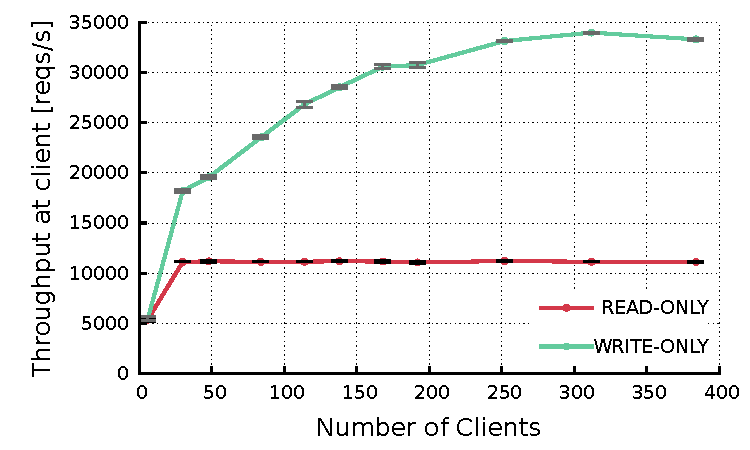
\includegraphics[width=0.5\linewidth]{../plots/baseline_nomidd_1server/THROUGHPUT.pdf}
		\label{Figure:baseline_nomidd_1server:a}}\hfill
	\subfloat[Response time]{%
		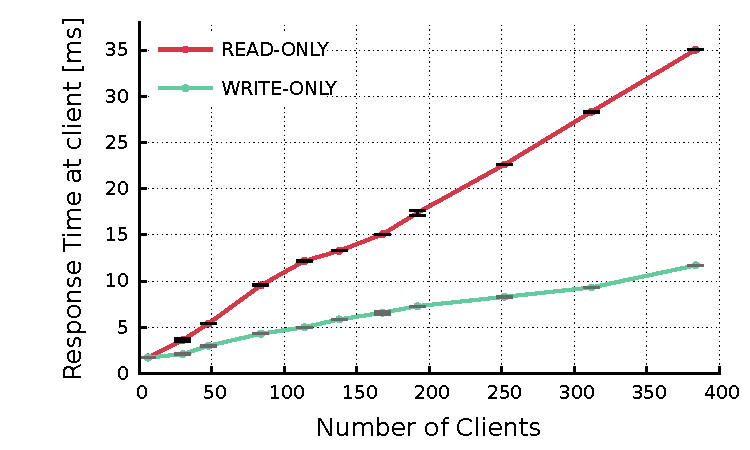
\includegraphics[width=0.5\linewidth]{../plots/baseline_nomidd_1server/RESPONSE_TIME.pdf}
		\label{Figure:baseline_nomidd_1server:b}}\\
	\caption{\textit{Baseline without middlewares, 3 memtier virtual machines and 1 memcached machine.} Mean throughput (a) and response times (b) measured at memtier client vs varying number of clients for both, read-only and write-only loads. Each point represents mean value between repetitions, and error bars illustrate one standard deviation between different repetitions.}
	\label{Figure:baseline_nomidd_1server} 	
\end{figure}

\begin{figure}[ht!]
	\centering	
	\subfloat[Under read-only load]{%
		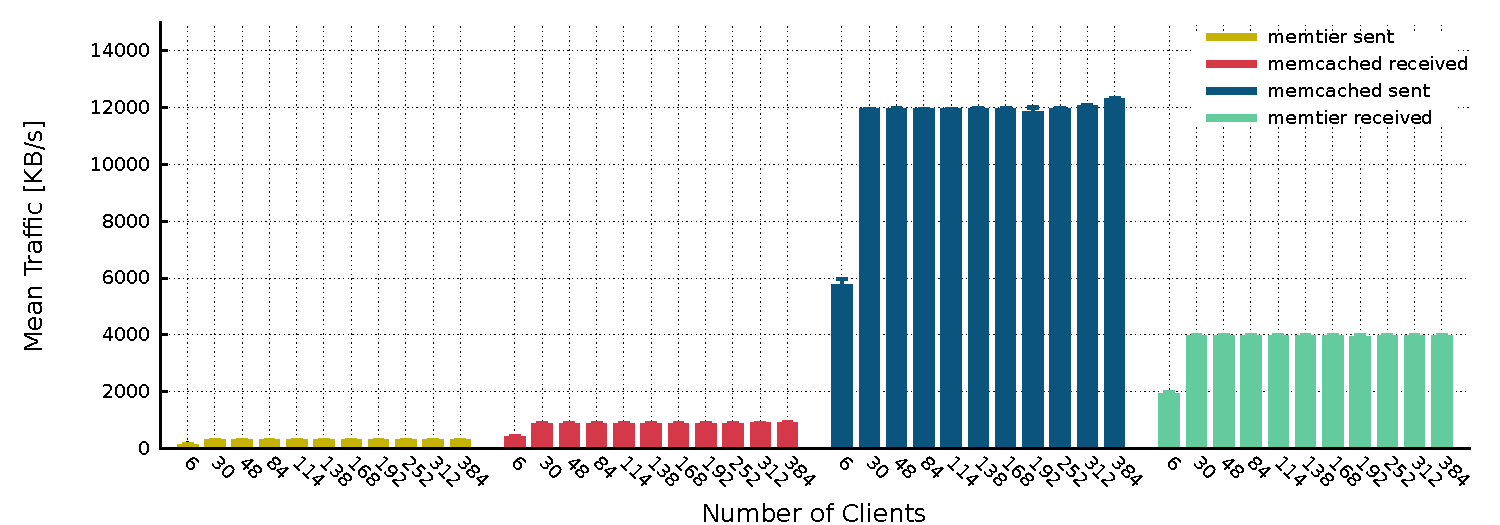
\includegraphics[width=1\linewidth]{../plots/baseline_nomidd_1server/NETWORK_READ-ONLY.pdf}
		\label{Figure:baseline_nomidd_1server_dstat:a}}\\
	\subfloat[Under write-only load]{%
		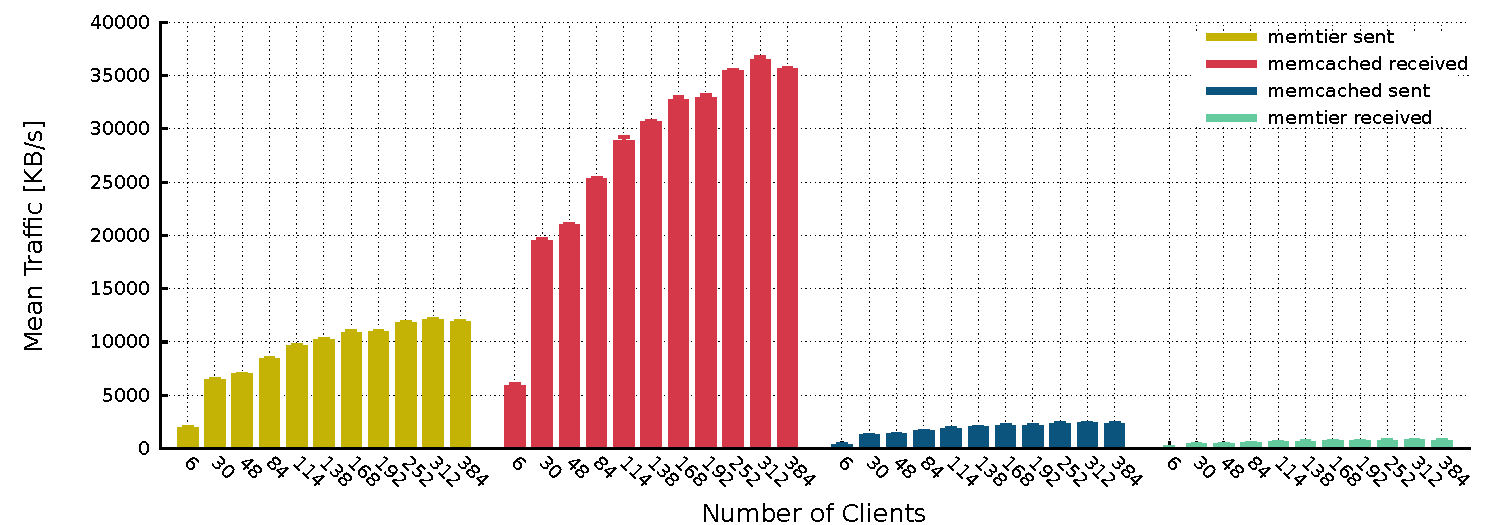
\includegraphics[width=1\linewidth]{../plots/baseline_nomidd_1server/NETWORK_WRITE-ONLY.pdf}
		\label{Figure:baseline_nomidd_1server_dstat:b}}\\
	\caption{\textit{Baseline without middlewares, 3 memtier virtual machines and 1 memcached machine.} Mean traffic \textbf{per virtual machine} measured at memtier and memcached side versus number of clients, illustrated for both loads. Error bars indicate one standard deviation between mean values over repetitions. Error bars are visible only above bars, but this confidence interval is symmetric.}
	\label{Figure:baseline_nomidd_1server_dstat} 	
\end{figure}

\subsubsection{Explanation}
Under read-only load (Figure \ref{Figure:baseline_nomidd_1server:a}), with increasing number of clients, throughput increases up to 30-clients load, but further increase in number of clients does not affect throughput in this case. On the other hand, for write-only load, throughput increases with increase in number of clients until 252 clients, after which throughput stabilizes. Response time (Figure \ref{Figure:baseline_nomidd_1server:b}) for read-only load grows faster with number of clients compared to response time under write-only load, which correlates to the throughput plot (higher response time under equal-client load leads to lower throughput).

In case of read-only load, with increase in number of clients (after 30 clients) throughput varies less than 1\%, but response time increases on average for 30\% between 2 consecutive number-of-client points, which clearly indicates that server was under-saturated until 30 clients, and is saturated afterwards. Under write-only load, from the beginning until 252-clients point, throughput has increased more than 5 times and response time has increased around 4 times, but afterwards throughput varies for 2\% while response times increases for 25\%. This means that the server was under-saturated until 252-clients point, when it reaches saturation.

Diagnostics with \texttt{dstat} tool provided Figure \ref{Figure:baseline_nomidd_1server_dstat} where average inbound and outbound traffic per memtier and memecached machine vs number of clients is illustrated. Under read-only load (Figure \ref{Figure:baseline_nomidd_1server_dstat:a}), each memtier machine sends around 300 KB/s and memcached machine receives around 900 KB/s which is 300 KB/s from each of memtier machines. Small outbound traffic from memtier machines is a result of short length of GET request (18 bytes) and the fact that memtier client is blocked until response is received. However, we can observe that increasing number of clients didn't increase outbound traffic at each of memtier machines. Reason for this lies at memcached machine: Outbound traffic of the memcached server reaches 12000 KB/sec, and given that length of GET response (with 1 key) is 1058 B, outbound troughput of (on average) 11614.37 GET responses per second is achieved, which is almost the limit outbound traffic for memcached machine (Table \ref{table:iperf}). This theoretical upper bound will never be achieved in this real-world scenario, but it is clear that server is the bottleneck in this setting (actually it's I/O operations and outbound bandwidth). Finally, one third of total server's outbound traffic is received by each of memtier machines.

Under write-only load (Figure \ref{Figure:baseline_nomidd_1server_dstat:b}), we can observe that maximal outbound traffic of memtier machines are around 12000 KB/s, which is half the theoretical upper-bound, so memtier machines are not bottleneck here. Furthermore, SET responses are only 8 B each (\texttt{STORED\textbackslash r\textbackslash n}), and the maximal outbound traffic of servers machine is not reached, so server's bandwidth is not the bottleneck as well. The bottleneck is actual server, which has only 1 user-thread (\texttt{-t 1}) to process all incoming traffic from clients. Moreover, \texttt{dstat} logs show higher cpu usage on server's machine than on clients' machines (for example, 20\% system and 15\% user cpu usage at server vs 8\% system and 6\% user cpu usage per client machine, for 192 clients in total), which leads to conclusion that server itself is the bottleneck under write-only load.

\subsection{Two Servers}

The individual parameters for this experiment are given in Table \ref{table:baseline_nomidd_2server:params}. Throughput and Response time as measured at memtier client are given in Figure \ref{Figure:baseline_nomidd_2server}.  Small error bars indicate that all experiments and repetitions were stable. Interactive Law holds for all experiments (e.g. for read-only load and $numclients=384$, average measured throughput is $X=20242.55333$reqs/s, and average measured response time is $R=9.48167$ms. By interactive law, response time should be $R_{il}=numclients/X=9.485$ms which is 0.33\% difference.).

\begin{center}
	\scriptsize{	
		\begin{table}[!ht]
			\centering
			\begin{tabulary}{\linewidth}{ | L | C |}
				\hline Number of servers	&	2	\\
				\hline Number of client machines	&	1	\\
				\hline Instances of memtier per machine	&	2	\\
				\hline Threads per memtier instance	&	1	\\
				\hline Virtual clients per thread	&	\{ 1, 5, 8, 13, 20, 27, 32, 42, 52, 64, 78, 96 \}	\\
				\hline Workload	&	Write-only and Read-only	\\
				\hline 
			\end{tabulary}
			\caption{\textit{Individual parameters for baseline experiment without middleware, 1 memtier client machine and 2 memcached server machines.}}
			\label{table:baseline_nomidd_2server:params}
		\end{table}
	}
\end{center}

\begin{figure}[ht!]
	\centering	
	\subfloat[Throughput]{%
		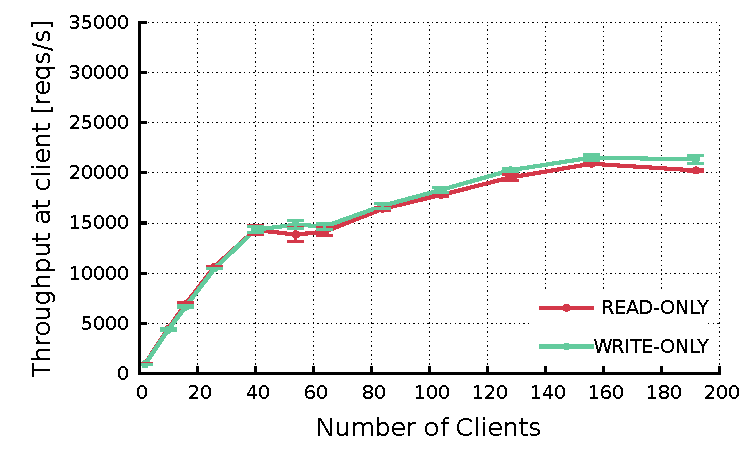
\includegraphics[width=0.49\linewidth]{../plots/baseline_nomidd_2servers/THROUGHPUT.pdf}
		\label{Figure:baseline_nomidd_2server:a}}\hfill
	\subfloat[Response time]{%
		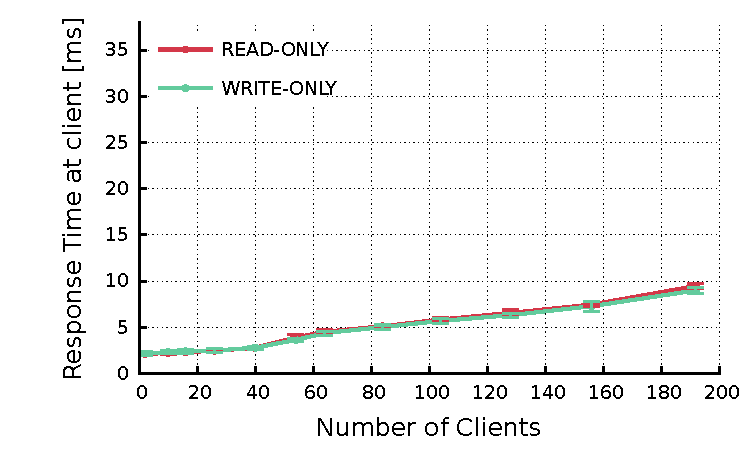
\includegraphics[width=0.49\linewidth]{../plots/baseline_nomidd_2servers/RESPONSE_TIME.pdf}
		\label{Figure:baseline_nomidd_2server:b}}\\
	\caption{\textit{Baseline without middleware, 1 memtier virtual machine and 2 memcached machines.} Mean throughput (a) and response times (b) measured at memtier client vs varying number of clients for both, read-only and write-only loads. Each point represents mean value between repetitions, and error bars illustrate one standard deviation between different repetitions.}
	\label{Figure:baseline_nomidd_2server} 	
\end{figure}

\begin{figure}[ht!]
	\centering	
	\subfloat[Under read-only load]{%
		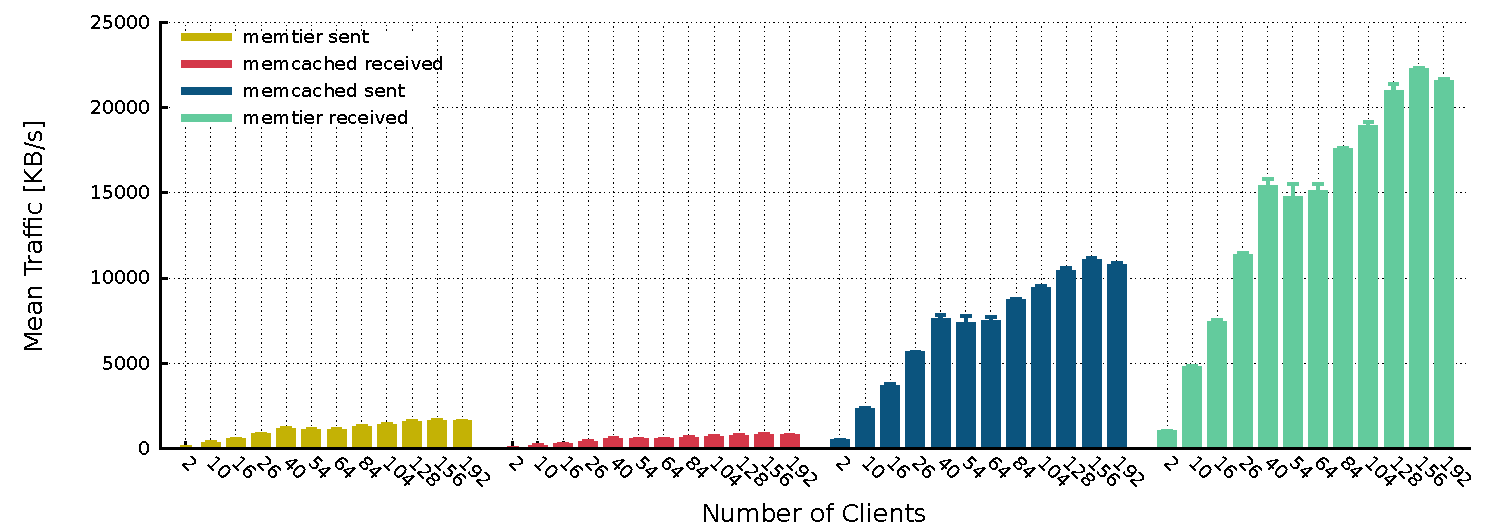
\includegraphics[width=1\linewidth]{../plots/baseline_nomidd_2servers/NETWORK_READ-ONLY.pdf}
		\label{Figure:baseline_nomidd_2server_dstat:a}}\\
	\subfloat[Under write-only load]{%
		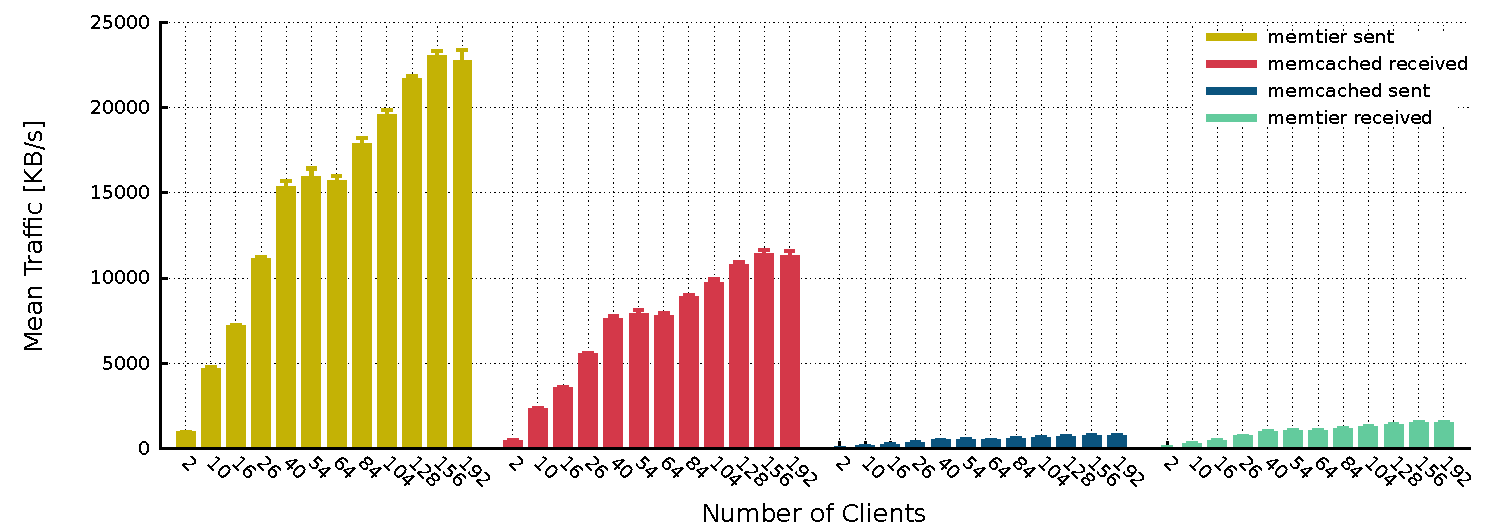
\includegraphics[width=1\linewidth]{../plots/baseline_nomidd_2servers/NETWORK_WRITE-ONLY.pdf}
		\label{Figure:baseline_nomidd_2server_dstat:b}}\\
	\caption{\textit{Baseline without middlewares, 1 memtier virtual machine and 2 memcached machines.} Mean traffic \textbf{per virtual machine} measured at memtier and memcached side versus number of clients, illustrated for both loads. Error bars indicate one standard deviation between mean values over repetitions. Error bars are visible only above bars, but this confidence interval is symmetric.}
	\label{Figure:baseline_nomidd_2server_dstat} 	
\end{figure}

\subsubsection{Explanation}

From Figure \ref{Figure:baseline_nomidd_2server} we can observe that throughput for both loads is very similar. In fact, system reaches saturation only at 156 clients for both loads, and until then system is under-saturated. During under-saturation phase (from 6 clients to 156 clients) throughput has increased 20.9 times and response time 2.56 times (which is 55\% and 13.9\% growth between every 2 consecutive client-loads on average, respectively), for both loads. In saturation phase, throughput is varying around 3\%, but response time increased 27\%, which clearly indicates saturation, for both loads.

Figure \ref{Figure:baseline_nomidd_2server_dstat} illustrates data obtained from \texttt{dstat} diagnostic tool. It illustrates inbound and outbound traffic \textbf{per machine} for both machine types and both load types. For read-only load (Figure \ref{Figure:baseline_nomidd_2server_dstat:a}), increasing number of clients resulted in increasing outbound traffic, which stabilized around 1600 KB/s, half of which is received by each of the memached machines. Each memcached server reaches it's upeer-limit for outbound traffic of 12000 KB/s during saturated phase, which controls throughput in this setting (throughput during saturated phase is double this limit, half from each of the servers). For this reason, the bottleneck of this setup under write-only load is the outbound bandwidth limit of servers machines. 

Under write-only load (Figure \ref{Figure:baseline_nomidd_2server_dstat:b}), increase in number of clients resulted in increase in outbound traffic that stabilized around 23000 KB/s during saturated phase. The reason for stabilization at this point is because upper-limit for outbound traffic at memtier machine is reached (Table \ref*{table:iperf}, this theoretical upper bound will never be reached in real-world setting because of all latencies and thinking times of machines). Logs from \texttt{dstat} show less than 15\% cpu usage at memtier, which verifies that machine has computational capabilities for higher performance, but is limited due to its outbound network bandwidth and I/O operations. For this reason, the bottleneck of this setup is limited maximal outbound bandwidth of clients machine. Half of memtier outbound traffic is received by each of memcached servers. Outbound traffic from memcached server machines is significantly lower due to the fact that size of SET response is only 8 B (\texttt{STORED\textbackslash r\textbackslash n}). Finally, inbound memtier machine traffic is double the outbound traffic from one server.

\subsection{Summary}

From the previous experiments, the following conclusions can be drawn:
\begin{itemize}
	\item Each memcached machine cannot process more than 11600 GET responses per second, and is bottleneck given sufficient read-only load. The bottleneck under write-only load is server itself, who runs on only 1 user-thread.
	\item Each memtier machine cannot generate more than 23000 SET requests per second, which is bottleneck assuming that server can handle this write-only load. Limitations on client's side regarding read-only load were not observed in given client range.
	\item One memcached server is saturated under read-only load with 30 clients, but saturates only with more than 252 clients under write-only load.
	\item Two memcached servers are saturated under read-only load with 156 clients, but for write-only load in second experiment bottleneck was memtier machine, reaching it's saturation with 156 clients as well.
\end{itemize}

Finally, maximal throughputs in first experiment are significantly different for two loads - throughput under read-only load is 3 times lower than under write-only load, and limitations are different as well: read-only load is bounded by maximal outbound bandwidth of server's machine, and write-only load by server itself, but not as strictly as read-only load. In second experiment however, throughputs for both loads are very similar, but as a result of different limiting factors: read-only load is again bounded by server's maximal outbound bandwidth and write-only load is bounded by outbound maximal bandwidth of memtier machine.

\begin{center}
	\scriptsize{	
		\begin{table}[ht!]
			\centering
			\begin{tabulary}{\linewidth}{ | L | C | C | C |}
				\hline	&	Read-only workload & Write-only workload & Configuration gives max. throughput	\\
				\hline One memcached server	&	11133.9 reqs/s	&	33.142.78 reqs/s	&	RO: 48 clients, WO: 252 clients	\\
				\hline One load generating VM	&	20906.7733 reqs/s	&	21526.67 reqs/s	&	both: 156 clients	\\
				\hline 
			\end{tabulary}
			\caption{\textit{Maximum throughput of different VMs.} Values are picked from the beginning of each of saturation phases. RO stands for Read-Only and WO stands for Write-Only}
			\label{table:baseline_nomidd:max_xput}
		\end{table}
	}
\end{center}


%%%%%%%%%%%%%%%%%%%%%%%%%%%%%%%%%%%%%%%%%%%%%%%%%%%%%%%%%%%%%%%%%%%%%%%%%%%%%%%%%%%%%%%%%%%%%%%%%%%%%%%%%
%%%%%%%%%%%%%%%%%%%%%%%%%%%%%%%%%%%%%%%%%%%%%%%%%%%%%%%%%%%%%%%%%%%%%%%%%%%%%%%%%%%%%%%%%%%%%%%%%%%%%%%%%
%%%%%%%%%%%%%%%%%%%%%%%%%%%%%%%  BASELINE WITH MIDDLEWARES
%%%%%%%%%%%%%%%%%%%%%%%%%%%%%%%%%%%%%%%%%%%%%%%%%%%%%%%%%%%%%%%%%%%%%%%%%%%%%%%%%%%%%%%%%%%%%%%%%%%%%%%%%
%%%%%%%%%%%%%%%%%%%%%%%%%%%%%%%%%%%%%%%%%%%%%%%%%%%%%%%%%%%%%%%%%%%%%%%%%%%%%%%%%%%%%%%%%%%%%%%%%%%%%%%%%

\section{Baseline with Middleware (90 pts)}

All middleware-related results presented here and in following sections were obtained offline. \texttt{Python} scripts process middleware logs in the following way: response times of all processed requests (by all workers in all middlewares) in each of the repetitions are averaged per 1 second window, and then averaged over stable-phase period resulting in 3 aggregates, one per each repetition. Final average and standard deviation of response time are calculated between these 3 values. Throughput is obtained in similar fashion, only throughputs of all workers and middlewares in each of repetitions are summed up. Every experiment in this report was run for 90 seconds, but first 10 seconds are considered warm-up phase and last 10 seconds are considered cool-down phase and results from these phases are not used in further calculations.

Before experiments, memcached server was pre-populated directly from memtier machine with following flags active: \texttt{--data-size=1024}, \texttt{--expiry-range = 9999-10000}, \texttt{--key-pattern = S:S} that iterates through keys sequentially making sure that server received at least one value for each of the possible keys, \texttt{--random-data} which generates bytes in value of SET requests uniformly at random. 

Because of the length of this experiment, for read-only load memcached server is populated with every change in number of clients.

%%%%%%%%%%%%%%%%%%%%%%%%%%%%%%%%%%%%%%%%%%%%%%%%%%%%%%%%%%%%%%%%%%%%%%%%%%%%%%%%%%%%%%%%%%%%%%%%%%%%%%%%%
%%%%%%%%%%%%%%%%%%%%%%%%%%%%%%%%%%%%%%%%%%%%%%%%%%%%%%%%%%%%%%%%%%%%%%%%%%%%%%%%%%%%%%%%%%%%%%%%%%%%%%%%%
%%%%%%%%%%%%%%%%%%%%%%%%%%%%%%%  BASELINE WITH 1 MIDDLEWARE
%%%%%%%%%%%%%%%%%%%%%%%%%%%%%%%%%%%%%%%%%%%%%%%%%%%%%%%%%%%%%%%%%%%%%%%%%%%%%%%%%%%%%%%%%%%%%%%%%%%%%%%%%
%%%%%%%%%%%%%%%%%%%%%%%%%%%%%%%%%%%%%%%%%%%%%%%%%%%%%%%%%%%%%%%%%%%%%%%%%%%%%%%%%%%%%%%%%%%%%%%%%%%%%%%%%

\subsection{One Middleware}

The goal of this section is to test and explain performance of the middleware. Parameters individual to this set of experiments are given in table \ref{table:baseline_1midd:params}. All experiments in this subsection are run on the same set of virtual machines.

\begin{center}
	\scriptsize{	
		\begin{table}[ht]
			\centering
			\begin{tabulary}{\linewidth}{ | L | C |}
				\hline Number of servers	&	1	\\
				\hline Number of client machines	&	1	\\
				\hline Instances of memtier per machine	&	1	\\
				\hline Threads per memtier instance	&	2	\\
				\hline Virtual clients per thread	&	\{ 1, 5, 8, 15, 22, 28, 32, 42, 52, 64 \}	\\
				\hline Workload	&	Write-only and Read-only	\\
				\hline Number of middlewares	&	1	\\
				\hline Worker threads per middleware	&	\{8, 16, 32, 64 \}	\\
				\hline 
			\end{tabulary}
			\caption{\textit{Individual parameters for baseline experiment with 1 middleware, 1 memtier client machine and 1 memcached server machine.}}
			\label{table:baseline_1midd:params}
		\end{table}
	}
\end{center}

\begin{figure}[ht]
	\centering	
	\subfloat[Mean queue size with read-only load]{%
		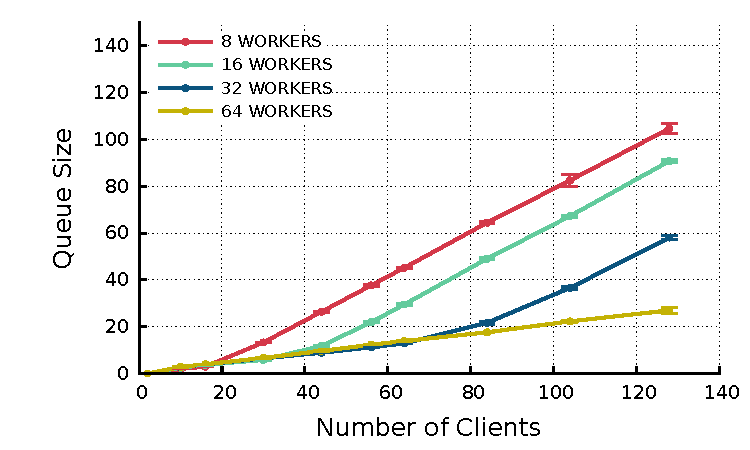
\includegraphics[width=0.49\linewidth]{../plots/baseline_1midd/timers/QUEUE_SIZE_READ-ONLY.pdf}
		\label{Figure:baseline_1midd_queue:a}}\hfill
	\subfloat[mean queue size with write-only load]{%
		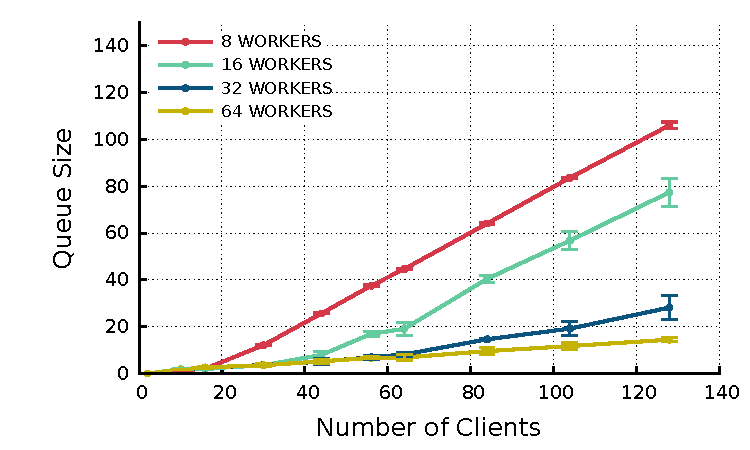
\includegraphics[width=0.49\linewidth]{../plots/baseline_1midd/timers/QUEUE_SIZE_WRITE-ONLY.pdf}
		\label{Figure:baseline_1midd_queue:b}}\\
	\caption{\textit{Baseline with 1 middleware machine, 1 memtier machine and 1 memcached machine.} Mean Queue size for different number of clients and workers for both loads.  Each point represents mean value between repetitions, and error bars illustrate one standard deviation between different repetitions.}
	\label{Figure:baseline_1midd_queue}	
\end{figure}

\begin{figure}[ht!]
	\centering	
	\subfloat[Throughput for read-only load]{%
		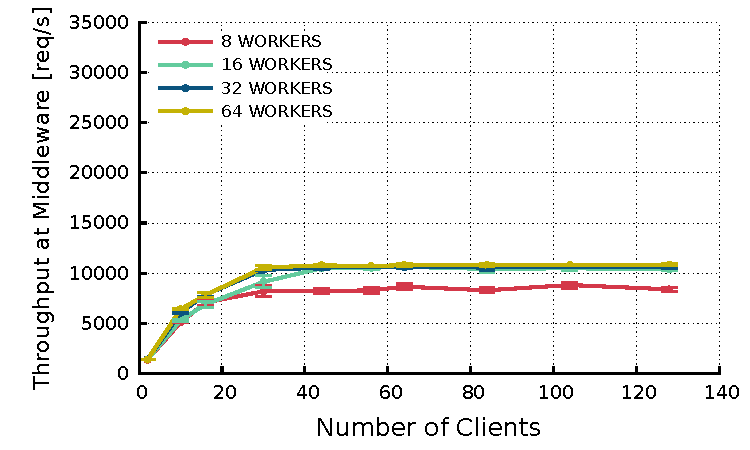
\includegraphics[width=0.49\linewidth]{../plots/baseline_1midd/timers/THROUGHPUT AT MIDDLEWARE - READ-ONLY.pdf}
		\label{Figure:baseline_1midd:a}}\hfill
	\subfloat[Throughput for write-only load]{%
		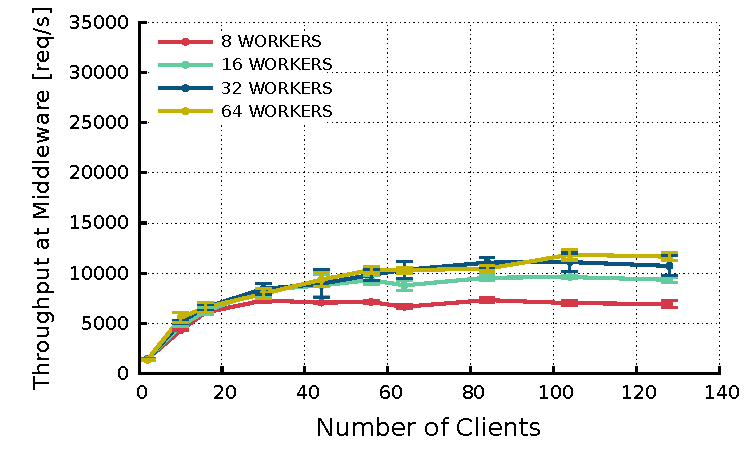
\includegraphics[width=0.49\linewidth]{../plots/baseline_1midd/timers/THROUGHPUT AT MIDDLEWARE - WRITE-ONLY.pdf}
		\label{Figure:baseline_1midd:b}}\\
	\subfloat[Response time for read-only load]{%
		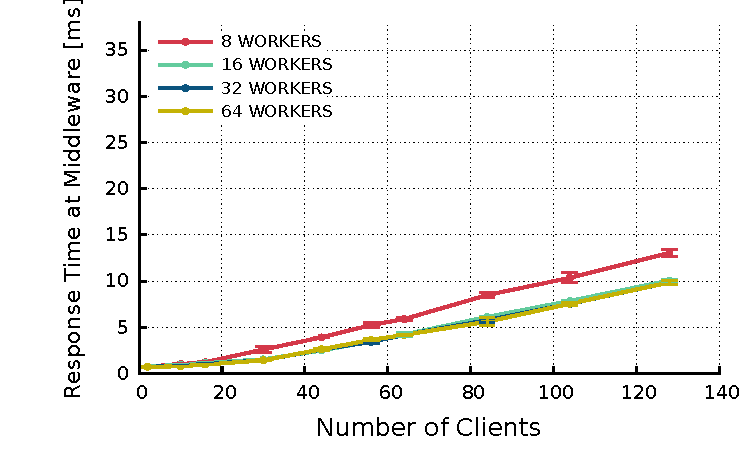
\includegraphics[width=0.49\linewidth]{../plots/baseline_1midd/timers/RESPONSE_TIME_READ-ONLY.pdf}
		\label{Figure:baseline_1midd:c}}\hfill
	\subfloat[Response time for write-only load]{%
		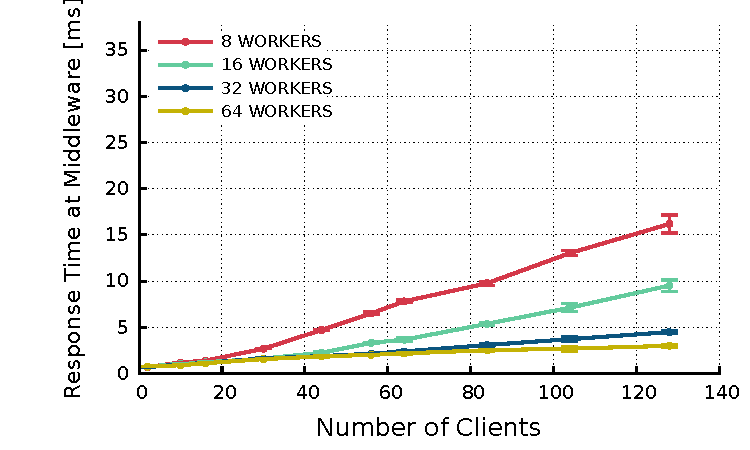
\includegraphics[width=0.49\linewidth]{../plots/baseline_1midd/timers/RESPONSE_TIME_WRITE-ONLY.pdf}
		\label{Figure:baseline_1midd:d}}\\
	\caption{\textit{Baseline with 1 middleware machine, 1 memtier machine and 1 memcached machine.} Mean throughput (a, b) and response times (c, d) measured at middleware vs varying number of clients for both, read-only and write-only loads and for 8, 16, 32 and 64 worker threads in middleware. Each point represents mean value between repetitions, and error bars illustrate one standard deviation between different repetitions.}
	\label{Figure:baseline_1midd}	
\end{figure}

\begin{figure}[ht!]
	\centering	
	\subfloat[Response times and its constituents for read-only load]{%
		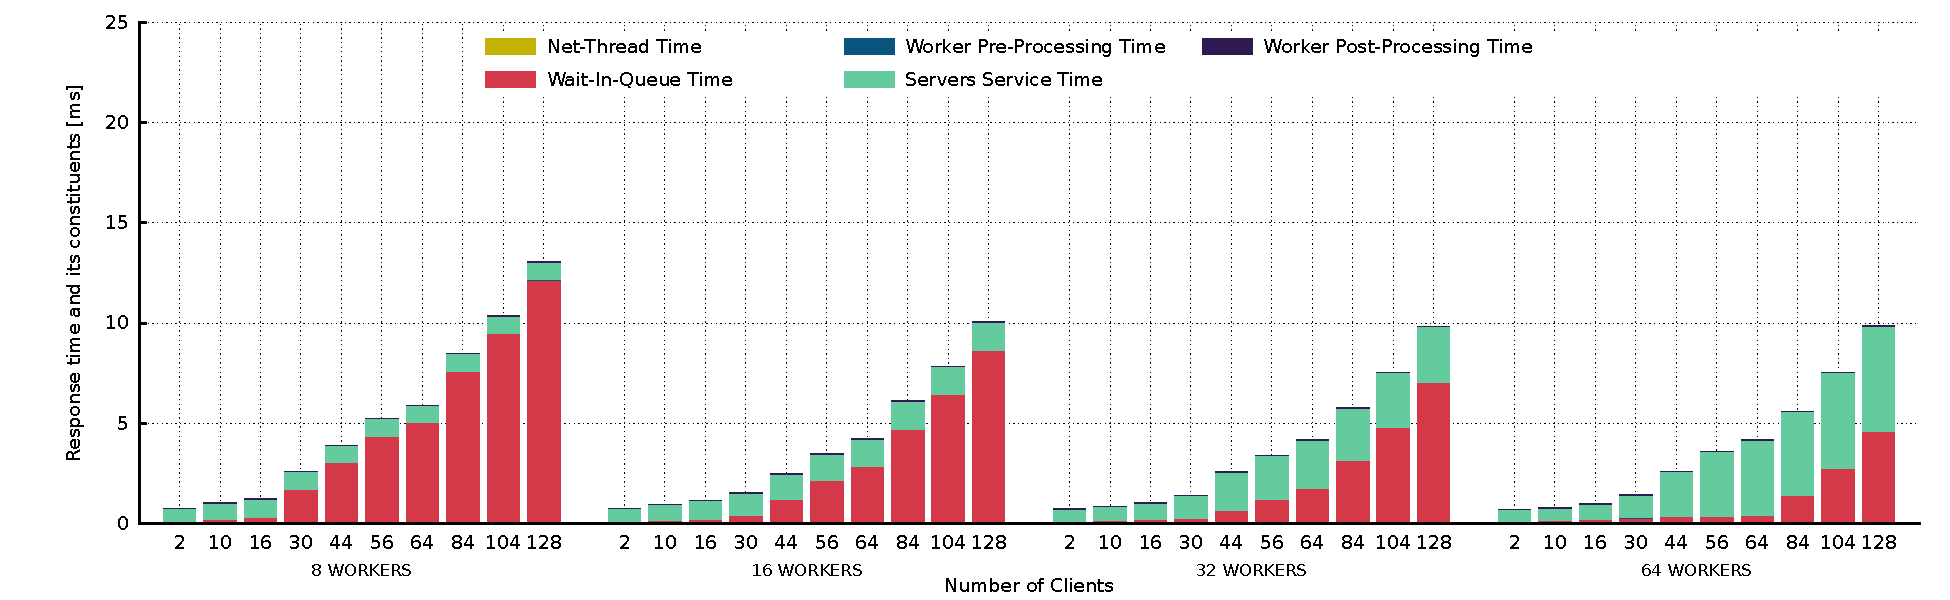
\includegraphics[width=1\linewidth]{../plots/baseline_1midd/timers/ALL_TIMES_TOGETHER_READ-ONLY.pdf}
		\label{Figure:baseline_1midd_all:a}}\\
	\subfloat[Response times and its constituents for write-only load]{%
		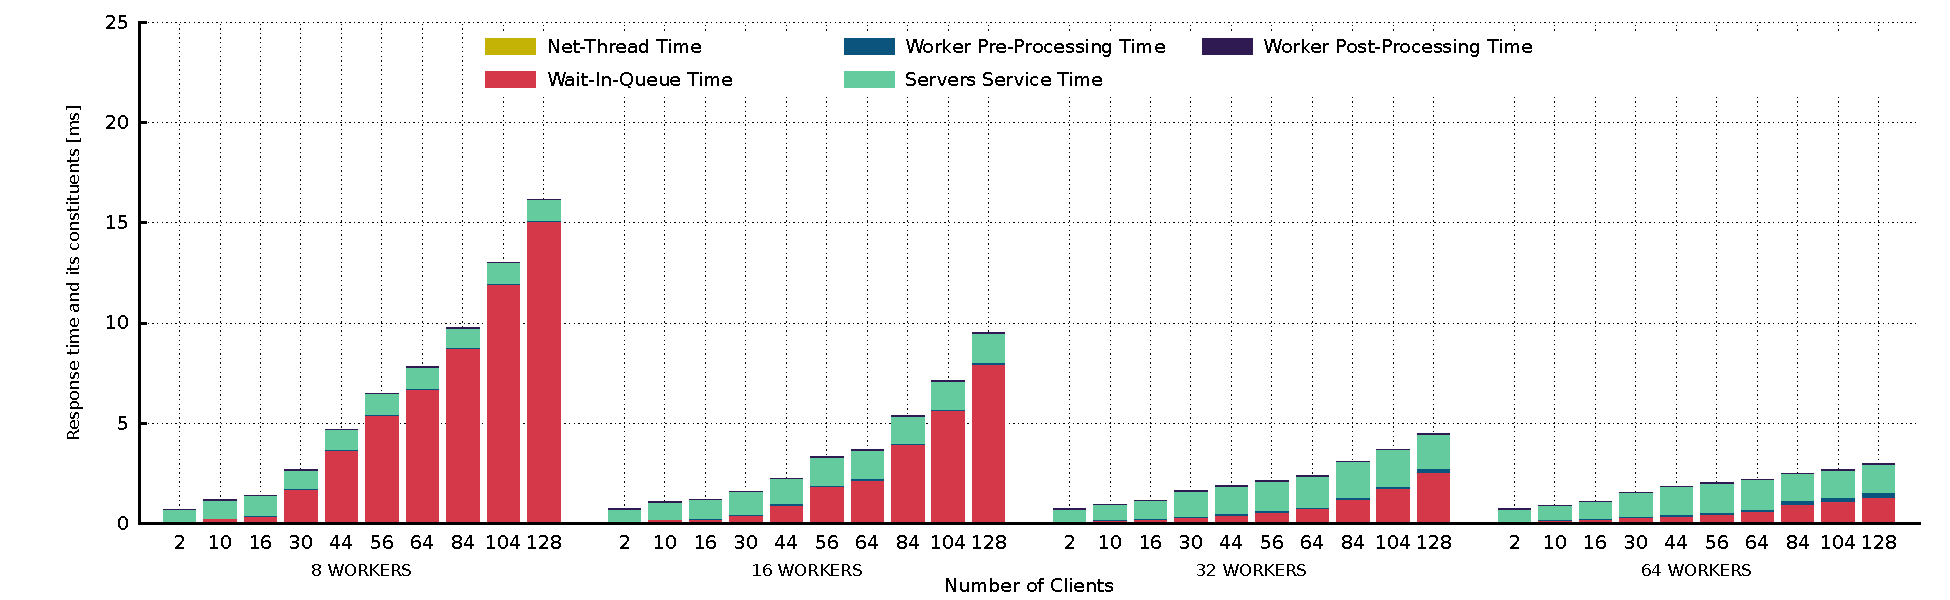
\includegraphics[width=1\linewidth]{../plots/baseline_1midd/timers/ALL_TIMES_TOGETHER_WRITE-ONLY.pdf}
		\label{Figure:baseline_1midd_all:b}}\\
	\caption{\textit{Baseline with 1 middleware machine, 1 memtier machine and 1 memcached machine.} Response time for different number of clients and workers for both loads, broken into constituents. Net-Thread processing time, worker pre-processing time and worker post-processing time are at all times lower than 1 ms, and therefore not visible on the plot.}
	\label{Figure:baseline_1midd_all}	
\end{figure}

\subsubsection{Explanation}

\textit{\textbf{Read-Only load.}} Increase in number of clients results in increase in throughput (Figure \ref{Figure:baseline_1midd:a}) but only to a point of 30-client-load, where system reaches saturation. For 8-workers configuration, the system saturates at a lower throughput than for the rest number of workers. This is because Net-Thread is faster at enqueueing requests than available workers are at dequeueing them. This can be verified in Figure \ref{Figure:baseline_1midd_all:a} - the most of the response time is spent waiting in the queue. 

Throughput for 16-, 32- and 64- client-configurations seems equal, which can be verified in Figure \ref{Figure:baseline_1midd:c}) where even response times for these configurations are equal. Throughput is fixed on the value corresponding to the maximal outbound bandwidth of memcached (A1) virtual machine, resulting in jobs waiting either in middleware's queue or server's. For lower number of workers (16), requests wait longer in the queue in the middleware, and jobs are processed in memcached with minimal server's queueing time up to the maximal available throughput. As number of workers increases, they are faster at dequeueing requests from middleware's queue, but now they are waiting at the server. This is illustrated in Figure \ref{Figure:baseline_1midd_all:a}. Finally, for configuration with 64 workers, request spends more time traveling to the server, being processed by the server and traveling back to the middleware than it spends waiting in the queue of the middleware.

Mean queue size plotted in Figure \ref{Figure:baseline_1midd_queue:a} follows break-down of response time illustrated in Figure \ref{Figure:baseline_1midd_all:a}: For 8 workers, requests wait longer in the queue because the queue contains more elements, but as number of workers is increased, requests are dequeued faster resulting in shorter queue length and shorter times spent waiting in it. Note that for 8-worker configuration, straight linear increase in queue length begins with 30-client-load, for 16-workers with 44-client load and for 32-worker configuration at 84-client load. At these points, time that requests spend in middelware's queue becomes longer than server service time. Queue-length-lines in the plot are parallel after these points, indicating that system is saturated. Finally, queue length for 64-workers configuration is fairly lower than for other configurations since, instead of waiting at the middleware, requests wait at the server.

To conclude, bottleneck of this system under read-only load is in middleware - increasing number of workers increases throughput, but only for 8-workers configuration. For the rest, the bottleneck is server's maximal outbound bandwidth. 

\textit{\textbf{Write-Only load.}} For 8-worker configuration, again there is not enough workers to support the load, leading to fast saturation (the system is saturated with only 30 clients) and low saturated throughput (Figure \ref{Figure:baseline_1midd:b}). For the rest worker-configurations, further increase in number of clients increases throughput and decreases response time (Figure \ref{Figure:baseline_1midd:d}). With 8 workers, after the 30-clients point, throughput varies less than 1\%, but response time increased 6 times until 128-client point. With 16 workers, 	throughput varies around 1.4\% after 44-client point, and response time increases 4.2 times. For these 2 configurations, we can say that saturation is reached with 30 and 44 clients respectively for 8 and 16 workers configuration. However, for 32 and 64 workers, situation is not as clear: after 64-client load, throughput seems stable ( vary for 1.36\% and 4.35\% ) but response time grows very slow (increased 1.88 and 1.37 times between 128-client and 64-client load). This suggests that maybe loads with more than 128 clients could increase throughput a little more.

In Figure \ref{Figure:baseline_1midd_all:b} break-down of response time shows that for low number of workers, requests spend majority of time waiting in middleware's queue - there is not enough workers to support the load and dequeueing from middleware's queue is slow resulting in requests waiting longer in the queue, but once dequeued, they get processed fast. As number of workers increases, requests are dequeued faster from middleware's queue, but are processed slower. More available workers push more requests to the server, and instead of waiting at the middleware, requests wait at the server to be processed. However, the response time still decreases with increase in number of workers. Another interesting thing we can observe from this plot is increase of worker pre-processing time as number of workers is increased. During this time, SET request is fully parsed, and with more workers it takes longer since more workers are still sharing same CPU resources resulting in more context switches and longer time that thread waits for the CPU. This was not visible in read-only load as GET requests are not parsed (only checked if final 5 bytes correspond to \texttt{END\textbackslash r\textbackslash n}), but just forwarded to the server.

Mean queue size (Figure \ref{Figure:baseline_1midd_queue:b}) follows response time (Figure \ref{Figure:baseline_1midd:d}). For 8- and 16- worker configuration, we can observe linear (and parallel) increase in queue size and for 32-worker configuration queue size is not yet parallel to the lines corresponding to 8 and 16 workers, but is close. For 64-worker configuration, queue size increases very slowly, indicating that with this configuration, the system could possibly handle more load efficiently.

Finally, throughput with 64 workers is always higher or equal to throughput with 32 workers, except for 84-clients load. After analyzing dstat (which showed no unexpected behavior of memcached and middleware machines) and ping logs, we can attribute this discrepancy to the network: average ping round-trip-time when experiment with 32 workers was run is 0.552ms and 0.932ms when experiment with 64 workers was run, which is 68.9\% increase.

To conclude, in this system under write-only load the bottleneck is number of worker threads since increasing their number improved both throughput and response time.


%%%%%%%%%%%%%%%%%%%%%%%%%%%%%%%%%%%%%%%%%%%%%%%%%%%%%%%%%%%%%%%%%%%%%%%%%%%%%%%%%%%%%%%%%%%%%%%%%%%%%%%%%
%%%%%%%%%%%%%%%%%%%%%%%%%%%%%%%%%%%%%%%%%%%%%%%%%%%%%%%%%%%%%%%%%%%%%%%%%%%%%%%%%%%%%%%%%%%%%%%%%%%%%%%%%
%%%%%%%%%%%%%%%%%%%%%%%%%%%%%%%  BASELINE WITH 2 MIDDLEWARES
%%%%%%%%%%%%%%%%%%%%%%%%%%%%%%%%%%%%%%%%%%%%%%%%%%%%%%%%%%%%%%%%%%%%%%%%%%%%%%%%%%%%%%%%%%%%%%%%%%%%%%%%%
%%%%%%%%%%%%%%%%%%%%%%%%%%%%%%%%%%%%%%%%%%%%%%%%%%%%%%%%%%%%%%%%%%%%%%%%%%%%%%%%%%%%%%%%%%%%%%%%%%%%%%%%%


\subsection{Two Middlewares}

Parameters individual to this set of experiments are given in table \ref{table:baseline_2midd:params}. All experiments in this subsection are run without deallocating virtual machines. Experiments with 2 client virtual machines are, however, run on different set of physical machines.

\begin{figure}[ht!]
	\centering	
	\subfloat[Throughput for read-only load]{%
		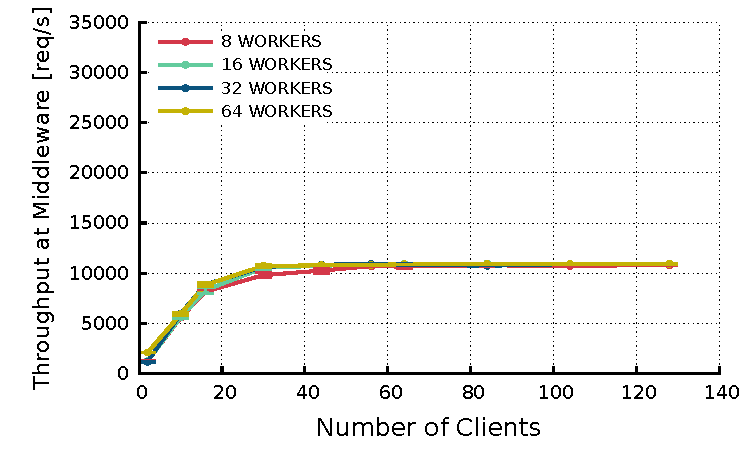
\includegraphics[width=0.49\linewidth]{../plots/baseline_2midd/timers/THROUGHPUT AT MIDDLEWARE - READ-ONLY.pdf}
		\label{Figure:baseline_2midd:a}}\hfill
	\subfloat[Throughput for write-only load]{%
		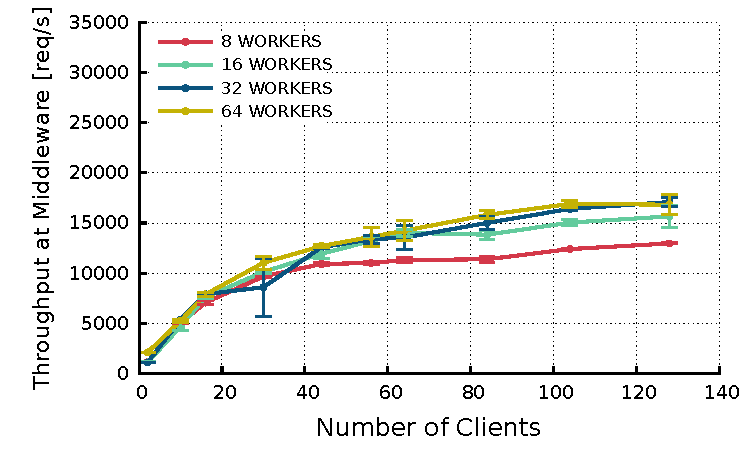
\includegraphics[width=0.49\linewidth]{../plots/baseline_2midd/timers/THROUGHPUT AT MIDDLEWARE - WRITE-ONLY.pdf}
		\label{Figure:baseline_2midd:b}}\\
	\subfloat[Response time for read-only load]{%
		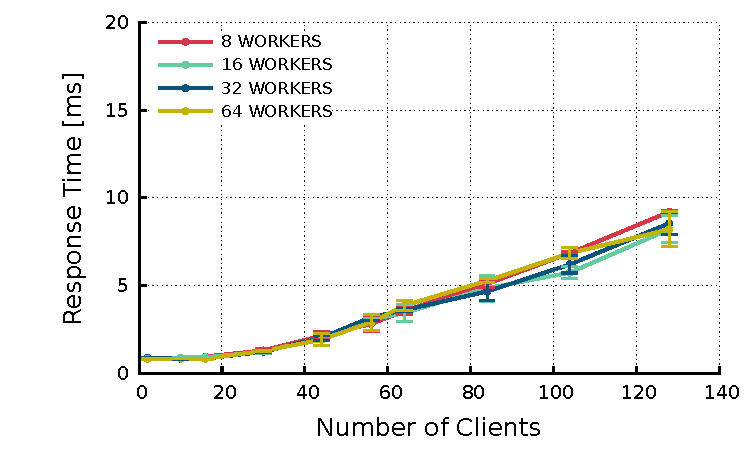
\includegraphics[width=0.49\linewidth]{../plots/baseline_2midd/timers/RESPONSE_TIME_READ-ONLY.pdf}
		\label{Figure:baseline_2midd:c}}\hfill
	\subfloat[Response time for write-only load]{%
		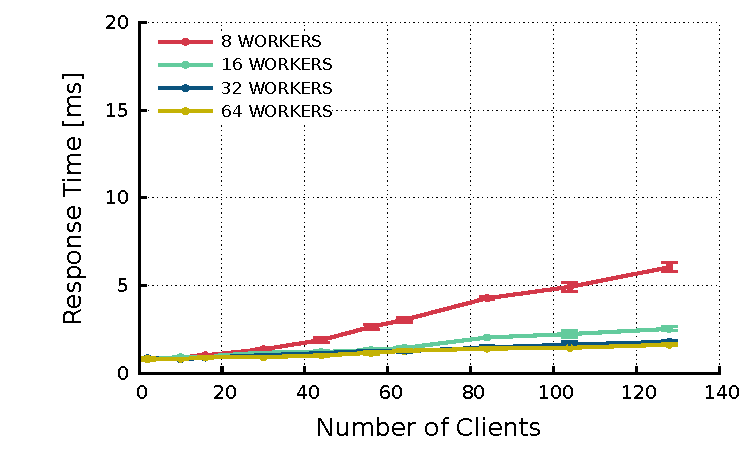
\includegraphics[width=0.49\linewidth]{../plots/baseline_2midd/timers/RESPONSE_TIME_WRITE-ONLY.pdf}
		\label{Figure:baseline_2midd:d}}\\
	\caption{\textit{Baseline with 2 middleware machines, 1 memtier machine and 1 memcached machine.} Mean throughput (a, b) and response times (c, d) measured at middlewares vs varying number of clients for both, read-only and write-only loads and for 8, 16, 32 and 64 worker threads in middleware. Each point represents mean value between repetitions, and error bars illustrate one standard deviation between different repetitions.}
	\label{Figure:baseline_2midd}	
\end{figure}

\begin{figure}[ht!]
	\centering	
	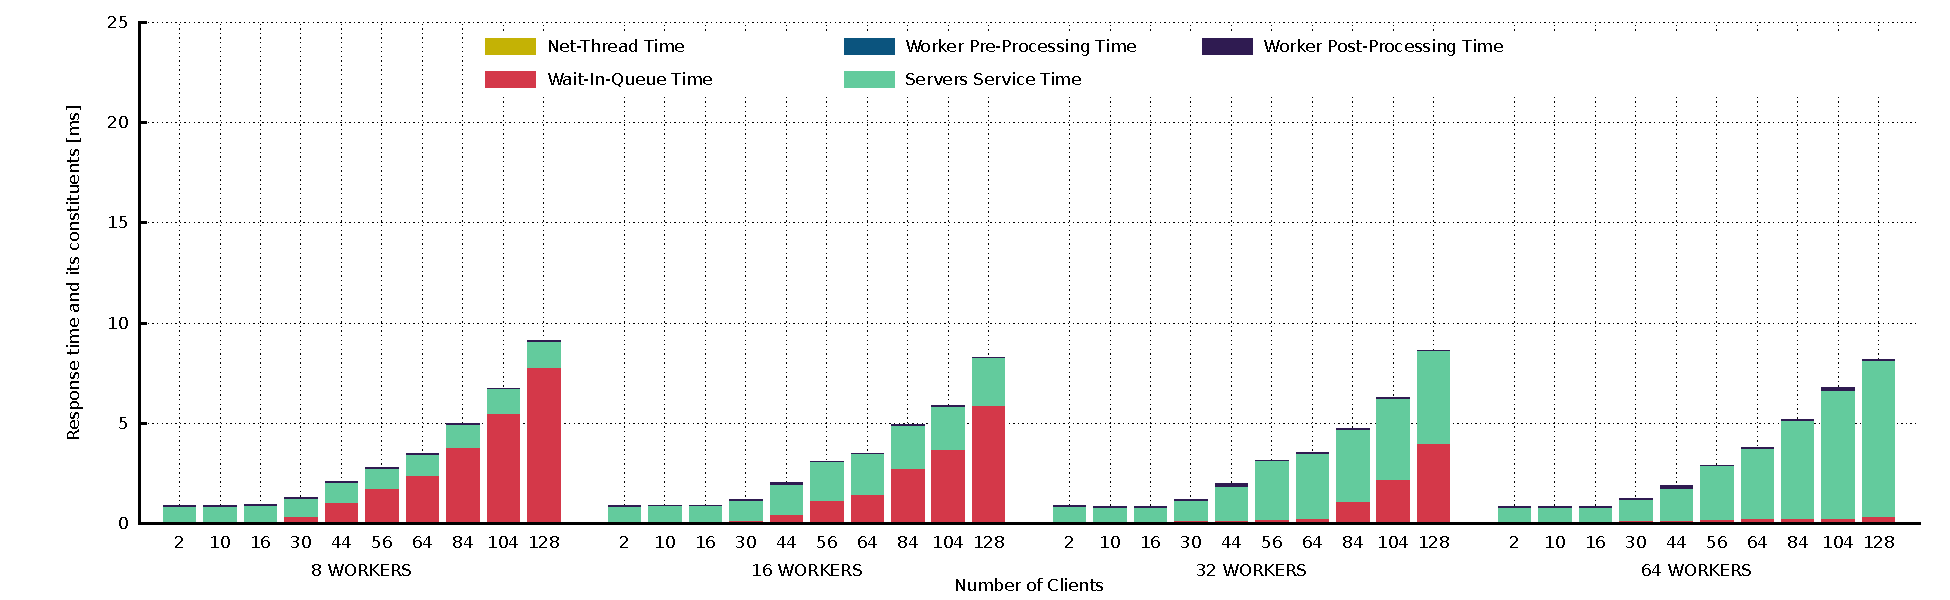
\includegraphics[width=1\linewidth]{../plots/baseline_2midd/timers/ALL_TIMES_TOGETHER_READ-ONLY.pdf}
	\label{Figure:baseline_2midd_all:a}\\
	\caption{\textit{Baseline with 1 middleware machine, 1 memtier machine and 1 memcached machine.} Response time for different number of clients and workers for read-only load, broken into constituents. Net-Thread processing time, worker pre-processing time and worker post-processing time are at all times lower than 1 ms, and therefore not visible on the plot.}
	\label{Figure:baseline_2midd_all}	
\end{figure}

\begin{figure}[ht!]
	\centering	
	\subfloat[Mean queue size with read-only load]{%
		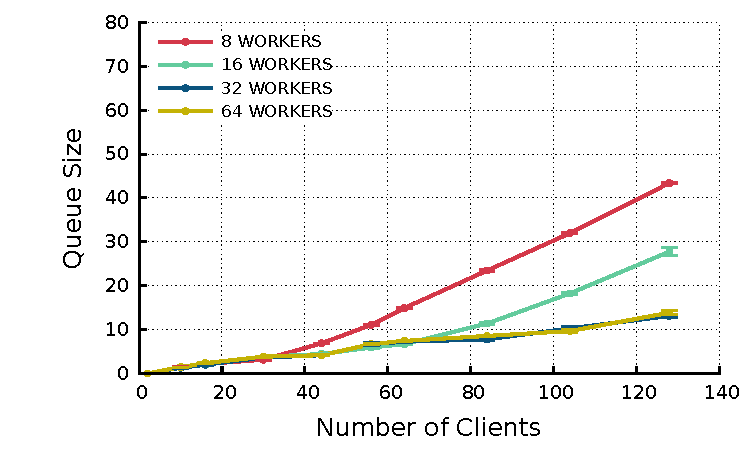
\includegraphics[width=0.49\linewidth]{../plots/baseline_2midd/timers/QUEUE_SIZE_READ-ONLY.pdf}
		\label{Figure:baseline_2midd_queue:a}}\hfill
	\subfloat[mean queue size with write-only load]{%
		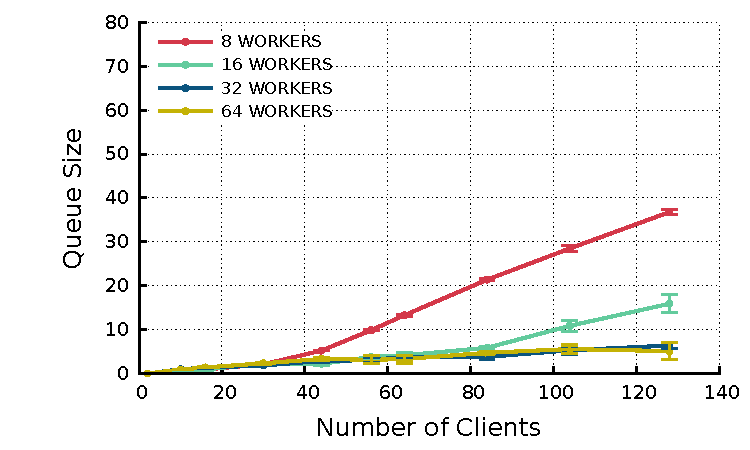
\includegraphics[width=0.49\linewidth]{../plots/baseline_2midd/timers/QUEUE_SIZE_WRITE-ONLY.pdf}
		\label{Figure:baseline_2midd_queue:b}}\\
	\caption{\textit{Baseline with 2 middleware machines, 1 memtier machine and 1 memcached machine.} Mean Queue size for different number of clients and workers for both loads.  Each point represents mean value between repetitions, and error bars illustrate one standard deviation between different repetitions.}
	\label{Figure:baseline_2midd_queue}	
\end{figure}

\begin{center}
	\scriptsize{	
		\begin{table}[!ht]
			\centering
			\begin{tabulary}{\linewidth}{ | L | C |}
				\hline Number of servers	&	1	\\
				\hline Number of client machines	&	1	\\
				\hline Instances of memtier per machine	&	2	\\
				\hline Threads per memtier instance	&	1	\\
				\hline Virtual clients per thread	&	\{ 1, 5, 8, 15, 22, 28, 32, 42, 52, 64 \}	\\
				\hline Workload	&	Write-only and Read-only	\\
				\hline Number of middlewares	&	2	\\
				\hline Worker threads per middleware	&	\{8, 16, 32, 64 \}	\\
				\hline 
			\end{tabulary}
			\caption{\textit{Individual parameters for baseline experiment with 2 middlewares, 1 memtier client machine and 1 memcached server machine.}}
			\label{table:baseline_2midd:params}
		\end{table}
	}
\end{center}

\subsubsection{Explanation}

\textbf{\textit{Read-Only load.}} Similar behavior is observed with 2 middlewares as was already observed in previous experiment. Throughput is again governed by the maximal bandwidth of the server. Increasing number of middlewares just improved throughput for 8-workers configuration, and response time for this configuration now follows response time of the rest. Figure \ref{Figure:baseline_2midd_all} verifies this: for low number of workers, dequeueing from middleware's queue is slow, but once dequeued, requests are processed fast. As number of workers increases, dequeueing from middleware's queue is faster, but now requests wait longer at the server. The bottleneck in this setup is, again, the maximal outbound bandwidth of server's machine, which controls and fixes throughput under any configuration to equal level. Saturation is reached already with 30 clients, as illustrated in Figure \ref{Figure:baseline_2midd:a}.

Mean queue size (Figure \ref{Figure:baseline_2midd_queue:a} shows mean size of both queues) is half the queue size from previous experiment which was to be expected since now there are 2 separate queues and equal load is now divided between them. Mean queue size increases faster for 8- and 16- worker configurations because they're slower at dequeueing than Net-thread is at enqueueing. On the other hand, mean queue size is very low for 32- and 16- worker configurations, since this many workers is fast at dequeueing requests, but requests wait longer at the server.

\textbf{\textit{Write-Only load.}} From Figure \ref{Figure:baseline_2midd:d} we can conclude that system is under-saturated in client range [0, 128] since response time remains almost constant (for 16, 32 and 64 workers) with increase in the load. This can also be seen in Figure \ref{Figure:baseline_2midd:b} where throughput doesn't seem to have reached saturation. Furthermore, mean queue size (Figure \ref{Figure:baseline_2midd_queue:b}) is also very low, especially with 32 and 64 workers. Given all aforementioned, this experiment is repeated with 2 client machines, only for write-only load. 

\subsubsection{Two middlewares with 2 client VMs}

Experiments in this subsection are not run on the same set of physical machines as experiments with 1 client machine and 2 middlewares. Only experiment under write-only load is repeated with 2 client machines, as for read-only load nothing would change since the bottleneck was outbound bandwidth of server's machine.

\begin{figure}[ht!]
	\centering	
	\subfloat[Mean throughput vs number of clients under write-only load]{%
		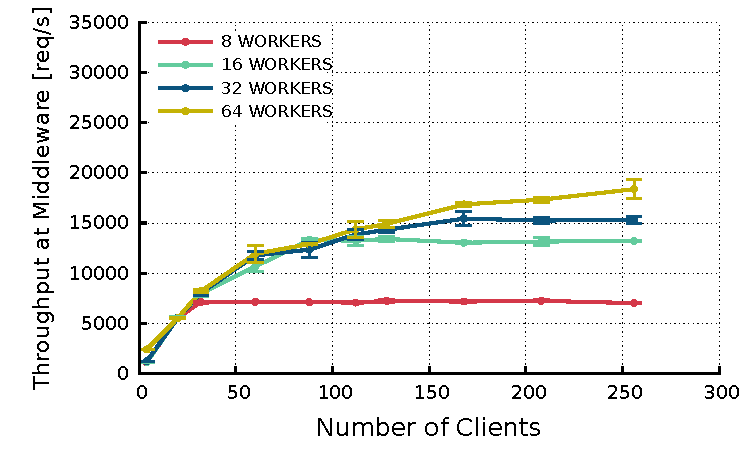
\includegraphics[width=0.49\linewidth]{../plots/baseline_2midd_2vms/timers/THROUGHPUT AT MIDDLEWARE - WRITE-ONLY.pdf}
		\label{Figure:baseline_2midd_2vms:a}}\hfill
	\subfloat[Mean response time vs number of clients uner write-only load]{%
		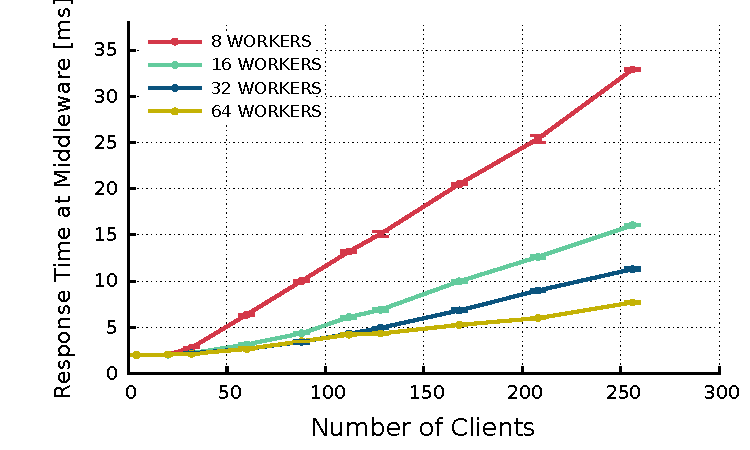
\includegraphics[width=0.49\linewidth]{../plots/baseline_2midd_2vms/timers/RESPONSE_TIME_WRITE-ONLY.pdf}
		\label{Figure:baseline_2midd_2vms:b}}\\
	\caption{\textit{Baseline with 2 middleware machines, 2 memtier machines and 1 memcached machine.}}
	\label{Figure:baseline_2midd_2vms}	
\end{figure}

\begin{figure}[ht!]
	\centering	
	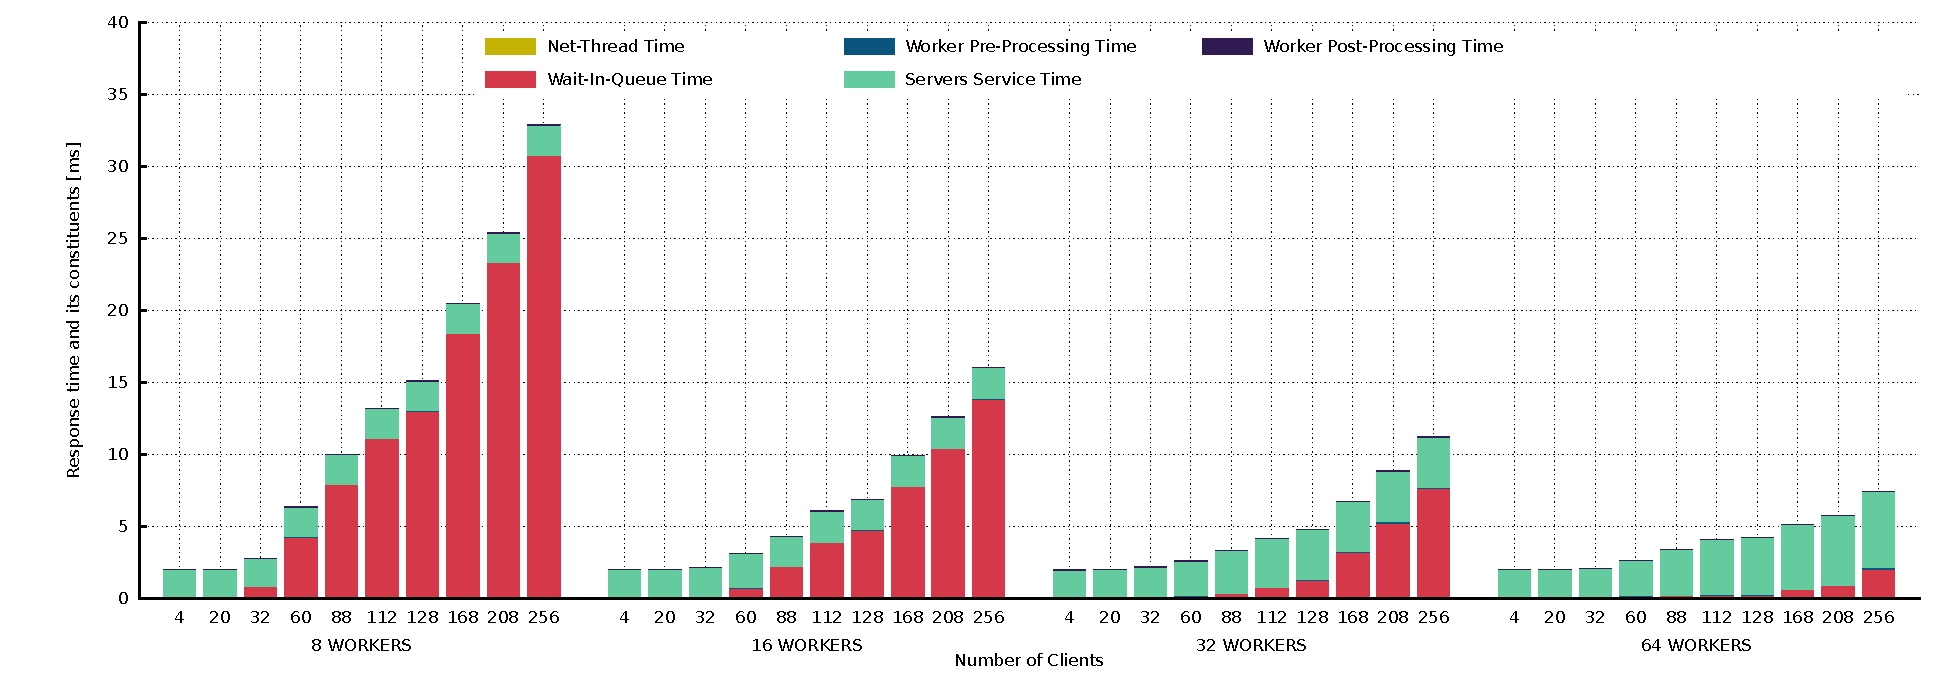
\includegraphics[width=1\linewidth]{../plots/baseline_2midd_2vms/timers/ALL_TIMES_TOGETHER_WRITE-ONLY.pdf}
	\label{Figure:baseline_2midd_2vms_all:a}\\
	\caption{\textit{Baseline with 2 middleware machines, 2 memtier machines and 1 memcached machine.} Response time for different number of clients and workers for write-only load, broken into constituents. Net-Thread processing time, worker pre-processing time and worker post-processing time are at all times lower than 1 ms, and therefore not visible on the plot.}
	\label{Figure:baseline_2midd_2vms_all}	
\end{figure}

\textit{\textbf{Write-Only load.}} As number of clients increases, throughput increases as well until saturation is reached: at 32-client load for 8 workers, 88-client load for 16 workers and 168-client load for 32 workers. In range of clients [0, 256] on 2 virtual machines, saturation is not reached for configuration with 64 workers, as both throughput and response time increase steadily with increasing load.

For low number of workers, requests again spend most of the time in middleware's queue, and as number of workers increases, response time decreases, requests spend less and less time in middleware's queue, but wait longer at the server. Here, more workers send more jobs to the server and the server takes longer time to process them. Analysis of \texttt{dstat} logs shows that user and system CPU usage are around 2.3\% and 3.2\% for 8-workers configuration, but for 64-workers respective values are 7.8\% and 9.99\%. Although these values are not large and there is room for improvement, let us remember that memcached has only 1 user thread (flag \texttt{-t 1}) to deal with all incoming jobs.

Finally, in this setup, the bottleneck is number of workers in the middleware, as most of the response time is spent waiting in middlewares' queues, and increasing number of workers improves both response time and throughput, until 64-worker configuration, where dominant amount of time is spent in traveling to the server and being processed at the server, in client range [0, 256]. However, as it was mentioned above, saturations has not been observed in this client range, and it is my guess that with increased load, the bottleneck would be insufficient number of workers.

\subsection{Summary}

\textit{\textbf{Read-Only load.}} As mentioned before, the bottleneck in both experiments (with 1 and 2 middlewares) is maximal outbound throughput of the server, and while throughput is fixed for increasing load, response time increases with the load. Therefore, maximal throughput values in the tables \ref{table:baseline_1midd:max_xput} and \ref{table:baseline_2midd:max_xput} correspond to configuration with 64 workers under load for which the flat part of throughput begins (44 client-load for both 1 and 2 middlewares). Adding a middleware did not change much in terms of throughput. Regarding response time, first we can observe a slight difference between response times measured on the client and ones measured on the middlewares. We can attribute this to network delay, since response time as measured on the client includes 2 traveling times between client and middleware and response time as measured on the middleware. Furthermore, aggregates provided by the client include warm-up and cool-down phases while aggregates measured on the middleware do not. This is why throughput at middleware is a bit higher than throughput measured on the client. Second, adding a middleware seems to decrease response times. Reported values occur for the same load, but in case with 2 middlewares, each of them receives half of it, and network between client and each of the middlewares is less utilized compared to the case with 1 middleware. This is especially important for sending responses back to the client as they are longer than GET requests. However, these 2 experiments were run on 2 different sets of physical machines, and comparing them might be unfair.

Finally, average time spent in middleware's queue is very short under max-thourghput configuration of 64 workers. This is because workers are fast at dequeueing, but requests are waiting longer at the server. Wait-in-queue time is halved as number of middlewares is doubled (equal load now goes to 2 different queues). Miss-rate is 0 since memcached is frequently populated before running experiments under read-only load.

\begin{center}
	\scriptsize{	
		\begin{table}[!ht]
			\centering
			\begin{tabulary}{\linewidth}{ | l | C | C | C | C |}
				\hline									&	Throughput [req/s]	&	Response Time [ms]	&	Average time in queue [ms]	&	Miss rate	\\
				\hline	Reads: Measured on middleware	&	10790.09	&	2.63	&	0.33	&	0.0	\\
				\hline	Reads: Measured on clients		&	10647.42	&	4.13	&	n/a		&	0.0	\\
				\hline	Writes: Measured on middleware	&	11842.02	&	2.69	&	1.02	&	n/a	\\
				\hline	Writes: Measured on clients		&	11740.03	&	8.85	&	n/a 	&	n/a	\\
				\hline 
			\end{tabulary}
			\caption{\textit{Max throughput for 1 middleware.}}
			\label{table:baseline_1midd:max_xput}
		\end{table}
	}
\end{center}

\textit{\textbf{Write-Only load.}} Maximal throughput reported in tables \ref{table:baseline_1midd:max_xput} and \ref{table:baseline_2midd:max_xput} correspond to the maximal observed mean throughput. In both experiments (with 1 and 2 middlewares) it occurs in configuration with 64 workers, but under different loads. It can seem that throughput has increased with increase in number of middlewares, but note that in experiment with 1 middleware, clear saturation with 64 workers has not been observed in client range [0, 128], and in second experiment the number of clients was doubled. However, for 128-client load in experiment with 1 middleware maximal throughput reached was 11648.67 req/s, but for the same load in experiment with 2 middlewares, throughput is 14907.17 reqs/s. Even though these 2 experiments were run on 2 different sets of physical machines, and in second one there were 2 memtier clients generating the load, we can accept conclusion that increasing number of middlewares increases write-only throughput, since increase is around 28\%.

SET requests are a little bit longer than 1 KB, and with large number of clients sending all of them to one net-thread results in not receiving full request in one packet. This behavior was observed during first run of the middleware on Azure machines, and required adding verification of received bytes to check if they represent complete request. If not, the bytes are left in \texttt{ByteBuffer}, Net-Thread moves to another \texttt{SocketChannel} and tries to read message from that client. Note that in one iteration of main loop, Net-Thread tries to serve all observed incoming messages from all the clients sequentially, but if the message is not complete, it must wait for some other iteration to be read fully and enqueued in the system. Partially received messages are clear indicator of high traffic in the network which results in longer waiting times of (partially received) messages in streams of \texttt{SocketChannel}-s, which cannot be measured by the middleware, but is captured by the client. 

For this reason, 128-client load split between 2 middlewares in second experiment leads to a better performance compared to the first experiment (14907.17 reqs.s vs 11648.67 req/s), as a result of having less messages between clients and each middleware. Reported maximal throughput for 2 middlewares was observed under 256-client load, which means that each middleware is hit by 128-client load, resulting in almost the same difference between response times measured at client and middleware in both experiments - around 6ms.

These longer waiting times before request is fully read by Net-Thread combined with 2 traveling times between clients and middleware(s) and the fact that reported values at middleware exclude warm-up and cool-down phase explain the somewhat large difference in response times measured at the client and the middleware. This behavior was not observed in read-only load because GET requests are very short compared to SET requests. Furthermore, throughput measurements were not affected by this as throughput is number of \textbf{completed} jobs in some time span, and time of completion was measured precisely by the middleware.

Finally, average time spent in middleware's queue seems to increase with increase in number of middlewares. However, difference is only 1 ms, experiments are run on 2 different sets of physical machines and max-throughput configuration is observed for different client-load, hence comparing these two values might be unfair. But, saturation with 64 workers under write-only load was not observed in either experiment and throughput per middleware is higher in second experiment which naturally increases wait-in-queue time.

\begin{center}
	\scriptsize{	
		\begin{table}[!ht]
			\centering
			\begin{tabulary}{\linewidth}{ | l | C | C | C | C |}
				\hline									&	Throughput [req/s]	&	Response Time [ms]	&	Average time in queue [ms]	&	Miss rate	\\
				\hline	Reads: Measured on middleware	&	10726.8		&	1.29	&	0.15	&	0.0	\\
				\hline	Reads: Measured on clients		&	10660.49	&	2.83	&	n/a		&	0.0	\\
				\hline	Writes: Measured on middleware	&	18372.19	&	7.68	&	2.02	&	n/a \\
				\hline	Writes: Measured on clients		&	18468.64	&	13.99	&	n/a 	&	n/a \\
				\hline 
			\end{tabulary}
			\caption{\textit{Max throughput for 2 middlewares.}}
			\label{table:baseline_2midd:max_xput}
		\end{table}
	}
\end{center}

%%%%%%%%%%%%%%%%%%%%%%%%%%%%%%%%%%%%%%%%%%%%%%%%%%%%%%%%%%%%%%%%%%%%%%%%%%%%%%%%%%%%%%%%%%%%%%%%%%%%%%%%%
%%%%%%%%%%%%%%%%%%%%%%%%%%%%%%%%%%%%%%%%%%%%%%%%%%%%%%%%%%%%%%%%%%%%%%%%%%%%%%%%%%%%%%%%%%%%%%%%%%%%%%%%%
%%%%%%%%%%%%%%%%%%%%%%%%%%%%%%%  THROUGHPUT FOR WRITES
%%%%%%%%%%%%%%%%%%%%%%%%%%%%%%%%%%%%%%%%%%%%%%%%%%%%%%%%%%%%%%%%%%%%%%%%%%%%%%%%%%%%%%%%%%%%%%%%%%%%%%%%%
%%%%%%%%%%%%%%%%%%%%%%%%%%%%%%%%%%%%%%%%%%%%%%%%%%%%%%%%%%%%%%%%%%%%%%%%%%%%%%%%%%%%%%%%%%%%%%%%%%%%%%%%%

\section{Throughput for Writes (90 pts)}

\subsection{Full System}

In this section, performance of middleware is tested in full system - 2 middlewares, 3 client machines and 3 server machines. Unlike previous write-only experiments, in full system SET requests are replicated and forwarded to all 3 servers. All experiments in this section were run without deallocating virtual machines. Individual parameters for this experiment are given in the Table \ref{table:writes:params}. 

\begin{center}
	\scriptsize{	
		\begin{table}[!ht]
			\centering
			\begin{tabulary}{\linewidth}{ | L | C |}
				\hline Number of servers	&	3	\\
				\hline Number of client machines	&	3	\\
				\hline Instances of memtier per machine	&	2	\\
				\hline Threads per memtier instance	&	1	\\
				\hline Virtual clients per thread	&	\{ 1, 5, 8, 15, 22, 28, 32, 42, 52, 64 \}	\\
				\hline Workload	&	Write-only	\\
				\hline Number of middlewares	&	2	\\
				\hline Worker threads per middleware	&	\{8, 16, 32, 64 \}	\\
				\hline 
			\end{tabulary}
			\caption{\textit{Individual parameters for "Throughput for Writes" experiment.}}
			\label{table:writes:params}
		\end{table}
	}
\end{center}

\begin{figure}[ht!]
	\centering	
	\subfloat[Mean Throughput at middleware]{%
		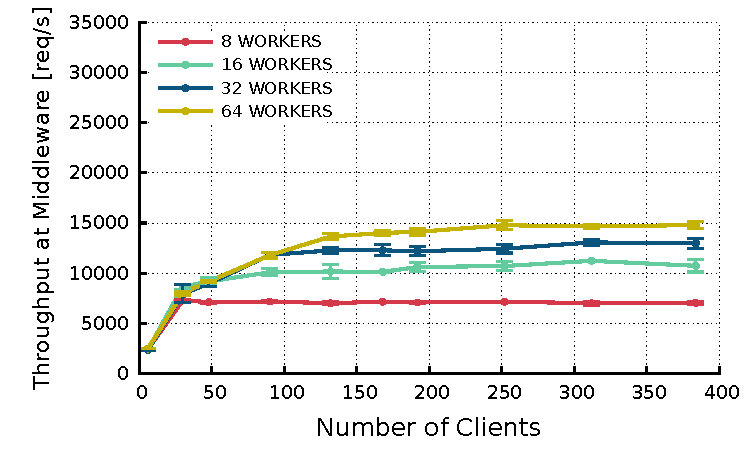
\includegraphics[width=0.49\linewidth]{../plots/experiment_write-only/timers/THROUGHPUT AT MIDDLEWARE - WRITE-ONLY.pdf}
		\label{Figure:experiment_write-only:a}}\hfill
	\subfloat[Mean Response time at middleware]{%
		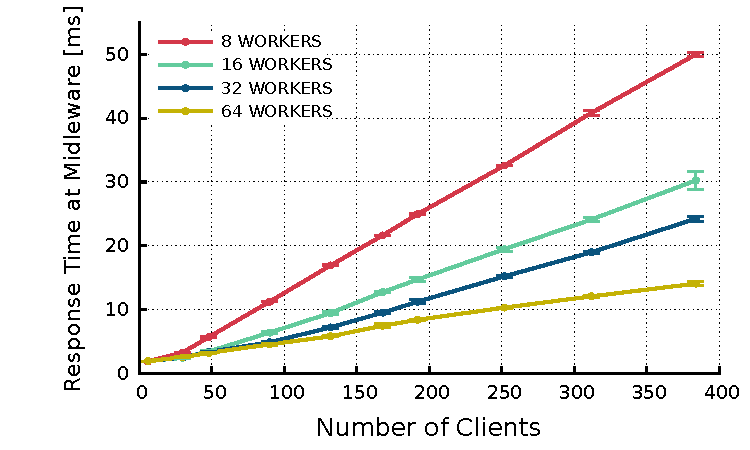
\includegraphics[width=0.49\linewidth]{../plots/experiment_write-only/timers/RESPONSE_TIME_WRITE-ONLY.pdf}
		\label{Figure:experiment_write-only:b}}\\
	\caption{\textit{Throughput for Writes} Mean throughput and response time as measured on the middleware vs number of clients.}
	\label{Figure:experiment_write-only}	
\end{figure}

\subsubsection{Explanation}

With increasing load, throughput (Figure \ref{Figure:experiment_write-only:a}) increases as well, until saturation is reached: at 48-clients load for 8 workers, at 90-clients load for 16, at 132-clients load for 32 workers and at 252-clients load for 64 workers. After these points throughput flattens out. Response time (\ref{Figure:experiment_write-only:b}) starts increasing significantly after these points as well.

Figure \ref{Figure:experiment_write-only_all} illustrates break-down of response time into constituents. For low number of workers, most of the time requests spend waiting in middleware's queue, and once dequeued, they are processed faster. As number of workers increases, wait-in-queue time in middleware decreases, but time spent traveling between middlewares and servers and processing time in servers increases. This is to be expected, as more workers push more requests towards servers resulting in longer processing times at server. However, for fixed number of workers, even with load increasing, server-service-time remains almost the same. This is because the bottleneck is middleware, more specifically number of workers who tend to keep requests in the queue of the middleware, thus controlling the load that servers need to process.

\begin{figure}[ht!]
	\centering	
	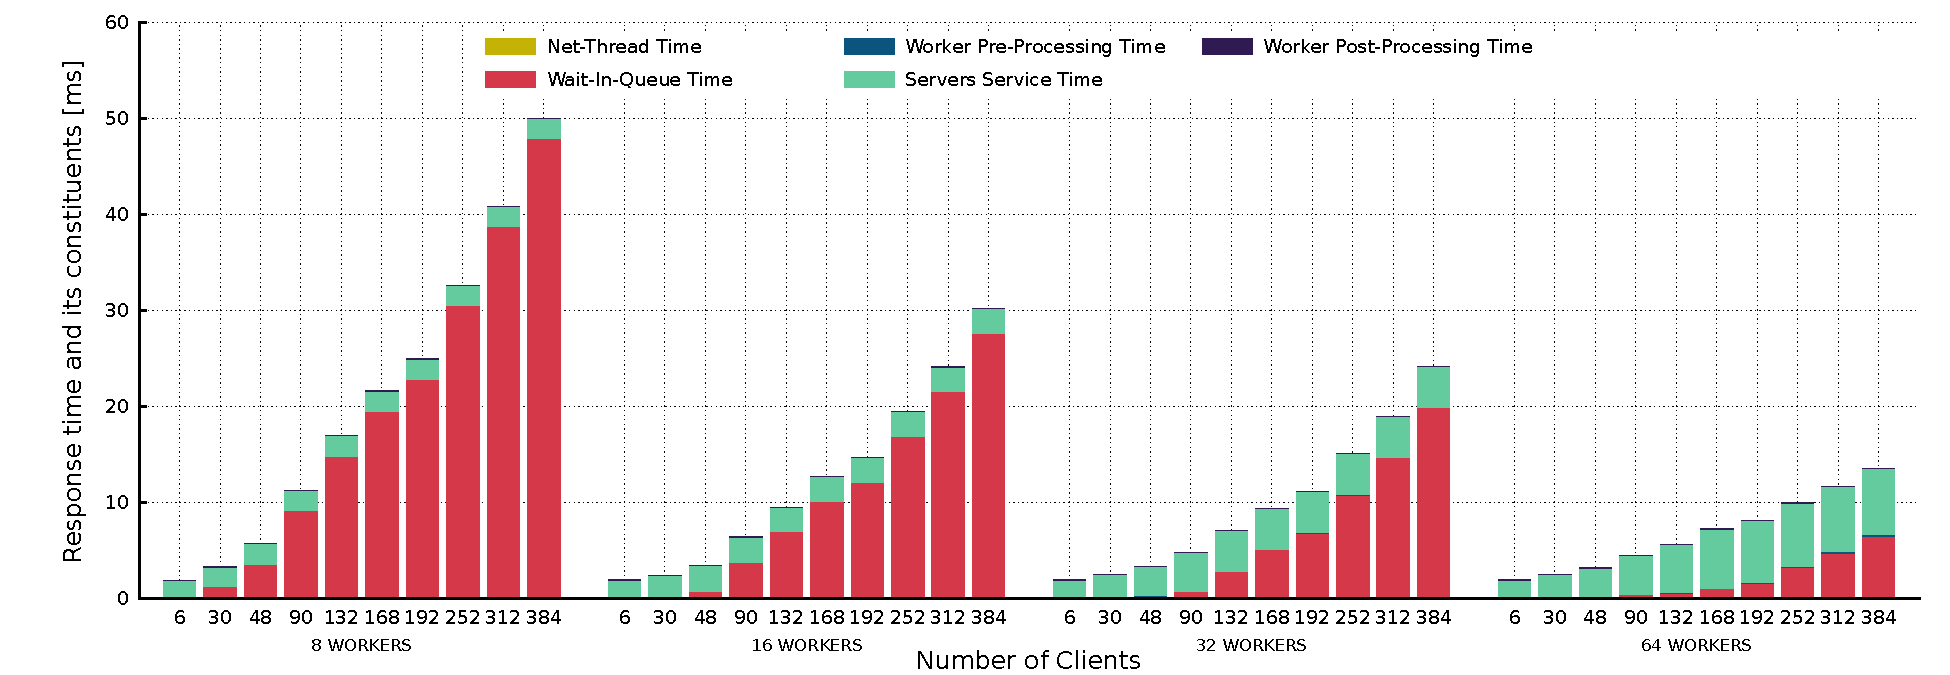
\includegraphics[width=1\linewidth]{../plots/experiment_write-only/timers/ALL_TIMES_TOGETHER_WRITE-ONLY.pdf}\\
	\caption{\textit{Throughput for Writes.} Response time for different number of clients and workers, broken into constituents. Net-Thread processing time, worker pre-processing time and worker post-processing time are at all times lower than 1 ms, and therefore not visible on the plot.}
	\label{Figure:experiment_write-only_all}	
\end{figure}

\subsection{Summary}

Values in the table correspond to mean throughput observed at the beginning of flat part of throughput (correspond to the points for which saturation is reached, and are mentioned above).
	
\begin{table}[!ht]
	\begin{adjustbox}{center}		
		\begin{tabulary}{\linewidth}{ | l | c | c | c | c |}
			\hline                                           			& 	\textbf{WT=8}	&	\textbf{WT=16}	&	\textbf{WT=32}		&	\textbf{WT=64} 		\\ 
			\hline \textbf{Throughput} [req/s] (Middleware)             			&	7121.35	&	10093.46	&	12275.80	&	14782.43	\\ 
			\hline \textbf{Throughput} [req/s] (Derived from MW response time)	&	8413.59	&	14028.95	&	18268.10	&	24416.38	\\ 
			\hline \textbf{Throughput} [req/s] (Client)                        	&	7232.32	&	10107.53	&	12066.8		&	14835.66	\\ 
			\hline \textbf{Average time in queue} [ms]							&	3.56	&	3.72		&	2.74		&	3.15		\\ 
			\hline \textbf{Average length of queue}                    			&	11.46	&	19.51		&	15.17		&	20.89       \\ 
			\hline \textbf{Average time waiting for memcached} [ms]				&	2.09	&	2.62		&	4.26		&	6.64       \\ 
			\hline 
		\end{tabulary}
	\end{adjustbox}
	\caption{\textit{Maximal Throughput for "Throughput for Writes" experiment.}}
	\label{table:writes:max_xput}
\end{table}

Increasing number of workers in the middlewares increases throughput. Throughputs as measured on the client and middleware are almost equal. Small differences come from the fact that aggregates on the client include warm-up and cool-down phase, but aggregates at middleware do not. Throughput derived from response time measured at middleware is significantly different than measured one. The reason, I believe, is the same as described in Summary of "Baseline with Middlewares" section. Average queue lengths are similar, as are times spent waiting in that queue (note that these values correspond to different client-loads, hence no pattern is observed\footnote{Queue size plot is available in repository and shows that queue length decreases with increase in number of workers.}). This is because points picked represent beginning of saturation phase, and similar state of the system (corresponding to available number of workers). If we model the system as closed network with $num of clients$ jobs circulating in it, then 23.87\%, 21.68\%, 11.49\% and 8.29\% of them are on average waiting in the queue, respectively for configuration with 8, 16, 32 and 64 workers. Time waiting for memcached or, as indicated in Figure \ref{Figure:experiment_write-only_all}, servers-service-time, increases as number of worker threads increases. As mentioned above, this is to be expected, since more workers push more load towards servers, and there is still only 1 thread per server to process all incoming traffic.

Finally, for all workers-configuration, bottleneck is insufficient number of workers in middleware.

%%%%%%%%%%%%%%%%%%%%%%%%%%%%%%%%%%%%%%%%%%%%%%%%%%%%%%%%%%%%%%%%%%%%%%%%%%%%%%%%%%%%%%%%%%%%%%%%%%%%%%%%%
%%%%%%%%%%%%%%%%%%%%%%%%%%%%%%%%%%%%%%%%%%%%%%%%%%%%%%%%%%%%%%%%%%%%%%%%%%%%%%%%%%%%%%%%%%%%%%%%%%%%%%%%%
%%%%%%%%%%%%%%%%%%%%%%%%%%%%%%%  GETS AND MULTI-GETS
%%%%%%%%%%%%%%%%%%%%%%%%%%%%%%%%%%%%%%%%%%%%%%%%%%%%%%%%%%%%%%%%%%%%%%%%%%%%%%%%%%%%%%%%%%%%%%%%%%%%%%%%%
%%%%%%%%%%%%%%%%%%%%%%%%%%%%%%%%%%%%%%%%%%%%%%%%%%%%%%%%%%%%%%%%%%%%%%%%%%%%%%%%%%%%%%%%%%%%%%%%%%%%%%%%%

\section{Gets and Multi-gets (90 pts)}

The purpose of this section is to test and explain performance of middleware(s) under mixed load with varying size of GET requests. All experiments in this section were run without deallocating virtual machines. Memtier clients were run using the same general flags mentioned before, with 2 differences: \texttt{--multi-key-get=}$N$ and \texttt{ratio=1:}$N$, where $N$ is number of keys in one GET request. This way, number of SET and GET messages is equal, only one GET message contains N keys. Individual parameters for this set of experiments are given in table \ref{table:gets:params}.

\begin{center}
	\scriptsize{	
		\begin{table}[!ht]
			\centering
			\begin{tabulary}{\linewidth}{ | L | C |}
				\hline Number of servers				&	3	\\
				\hline Number of client machines		&	3	\\
				\hline Instances of memtier per machine	&	2	\\
				\hline Threads per memtier instance		&	1	\\
				\hline Virtual clients per thread		&	2	\\
				\hline Multi-Get behavior               & sharded and non-sharded  \\
				\hline Multi-Get size                   & $N$ = {1, 3, 6, 9}   \\
				\hline Workload							&	1:$N$	\\
				\hline Number of middlewares			&	2	\\
				\hline Worker threads per middleware	&	64	\\
				\hline 
			\end{tabulary}
			\caption{\textit{Individual parameters for "Gets and Multi-gets" experiment.}}
			\label{table:gets:params}
		\end{table}
	}
\end{center}

\begin{figure}[ht!]
	\centering	
	\subfloat[Response time in non-sharded case]{%
		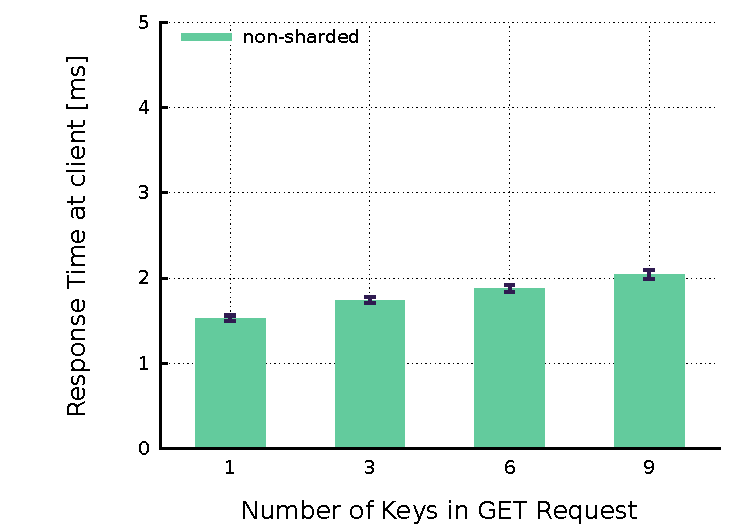
\includegraphics[width=0.49\linewidth]{../plots/experiment_gets/RESPONSE_TIME_NONSHARDED.pdf}
		\label{Figure:experiment_gets:a}}\hfill
	\subfloat[Response time in sharded case]{%
		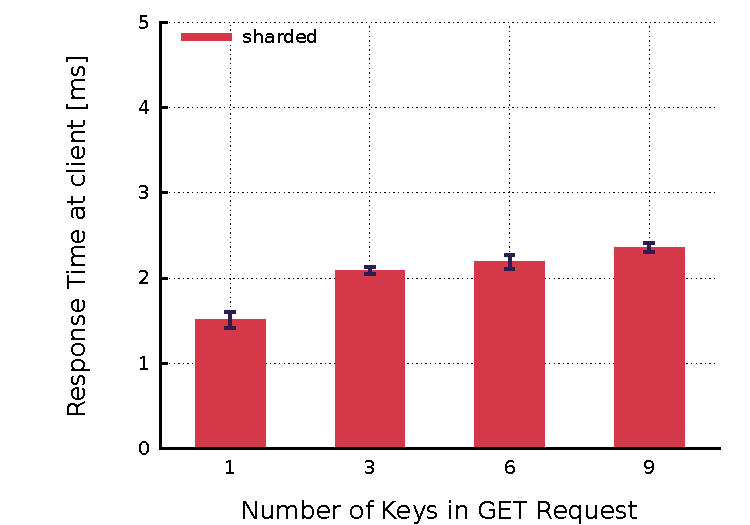
\includegraphics[width=0.49\linewidth]{../plots/experiment_gets/RESPONSE_TIME_SHARDED.pdf}
		\label{Figure:experiment_gets:b}}\\
	\caption{\textit{Experiment with GETs and multi-GETs.} Mean response time vs number of keys in GET request in both, sharded and non-sharded case. Error bars show 1 standard deviation between repetitions.}
	\label{Figure:experiment_gets}	
\end{figure}

\subsection{Sharded Case}

With sharding activated, GET request with multiple keys is divided into smaller GET requests, one for each server. Examples of sharding are given in table \ref{(Table:sharding_example)}.

\begin{figure}[ht!]
	\centering	
	\subfloat[Percentiles without sharding]{%
		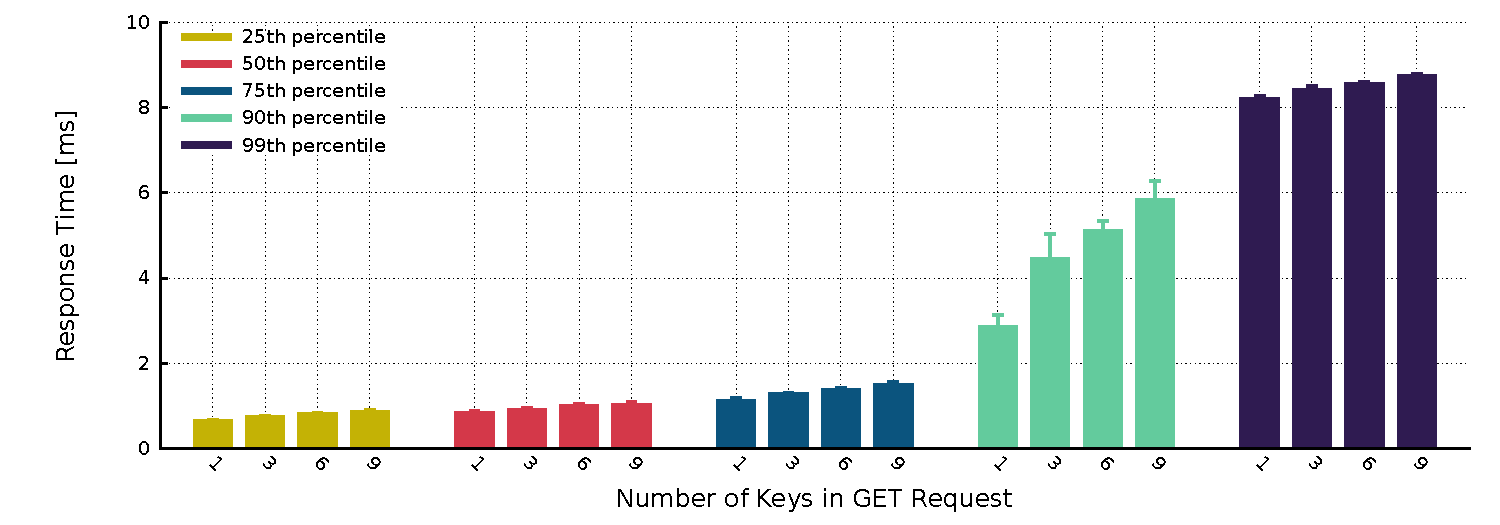
\includegraphics[width=1\linewidth]{../plots/experiment_gets/PERCENTILES_NONSHARDED.pdf}
		\label{Figure:experiment_gets_all:a}}\\
	\subfloat[Percentiles with sharding]{%
		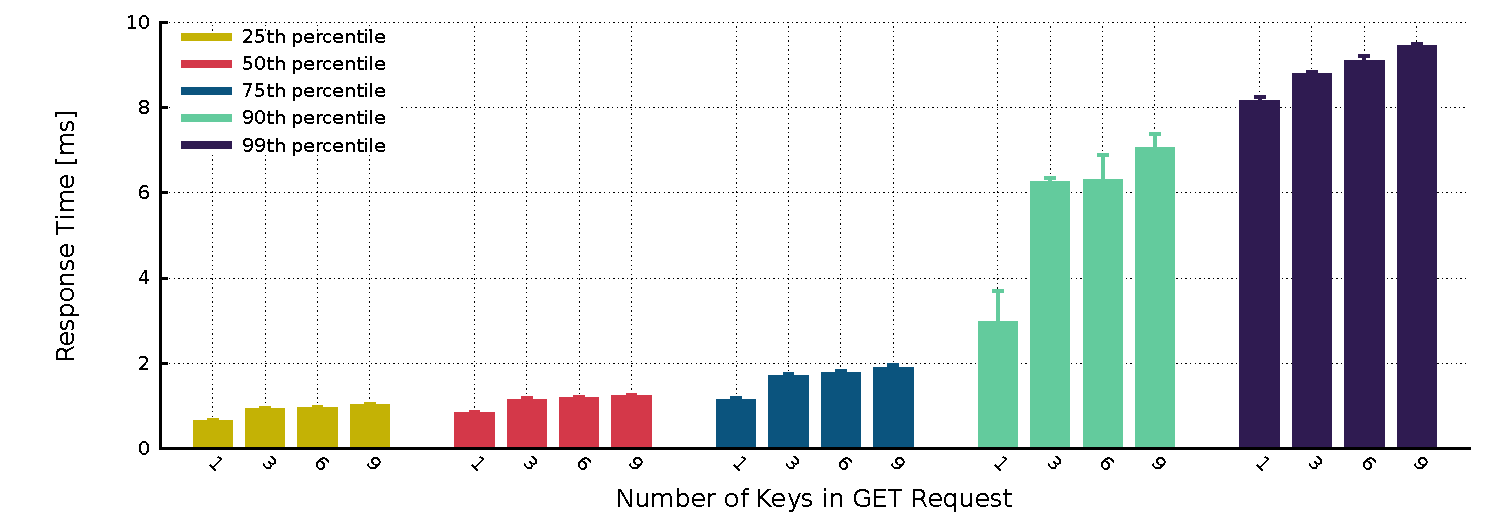
\includegraphics[width=1\linewidth]{../plots/experiment_gets/PERCENTILES_SHARDED.pdf}
		\label{Figure:experiment_gets_all:b}}\\
	\caption{\textit{Experiment with GETs and multi-GETs.} 25\textsuperscript{th}, 50\textsuperscript{th}, 75\textsuperscript{th}, 90\textsuperscript{th} and 99\textsuperscript{th} percentiles for response time as measured on the client vs number of keys in GET request. Error bars show one standard deviation between repetitions.}
	\label{Figure:experiment_gets_all}	
\end{figure}

\subsubsection{Explanation}

Response time vs number of keys in GET message is illustrated in Figure \ref{Figure:experiment_gets:b}, and we can observe that it increases as number of keys per request increases, and is significantly higher for GET messages with more than 1 keys. GET message with 1 key does not require splitting. Therefore, it is forwarded to 1 chosen server as it is. On the other hand, GET message with 3, 6 and 9 keys is divided in such a way that each server receives 1, 2 and 3 keys respectively. More keys require more processing time at middleware, which we can observe in Figure \ref{Figure:experiment_gets_break-down} as increase in worker post-processing time that is spent in assembling responses. But more importantly, more keys result in higher server-service time (Figure \ref{Figure:experiment_gets_break-down}) which includes 2 travel times between middleware and servers and processing on server. The reason for this, I believe, is that responses are not received in one packet since their size is 1 KB, 2 KB and 3KB for 1, 2 and 3 keys per request received by the server, respectively.

Response time percentiles, as measured on the client, are showcased in Figure \ref{Figure:experiment_gets_all:b}. Note that percentile data provided by memtier clients is organized by time (starting from 0 and incrementing response time in steps of 0.01ms, number of requests having response time lower or equal to it is calculated), so calculating exact percentile was not possible. However, granularity of client data was sufficient to find requested percentiles in $\pm$ 0.5\% range. From Figure \ref{Figure:experiment_gets_all:b} we can observe that 25\textsuperscript{th}, 50\textsuperscript{th} and 75\textsuperscript{th} percentiles for requests with 1 key are lower than for the rest. As mentioned before, it is expected, as no sharding takes place in this case. Interestingly, 25\textsuperscript{th}, 50\textsuperscript{th} and 75\textsuperscript{th} percentile in cases with 3, 6 and 9 keys per request are almost equal (per percentile) and all below 2ms. However, 90\textsuperscript{th} and 99\textsuperscript{th} percentiles are significantly higher. For 99\textsuperscript{th} percentiles, differences between number of keys are even more visible, but 99\% of jobs are finished in under 10ms. Possible reasons for this are discussed in "Histogram" subsection.

From Figure \ref{Figure:experiment_gets_break-down} we can observe that, on average, request spends the most time in traveling between middleware and server and being processed by servers, and wait-in-queue time is very low. Hence, we can conclude that system is not saturated and the bottleneck with this (\#client, \#worker) configuration is on servers' side (including network between middleware and servers). Note also that total response time as measured on the middleware (\ref{Figure:experiment_gets_break-down}) is lower than as measured on the client (\ref{Figure:experiment_gets:b}), due to additional traveling time between middleware and clients.

\begin{figure}[ht!]
	\centering	
	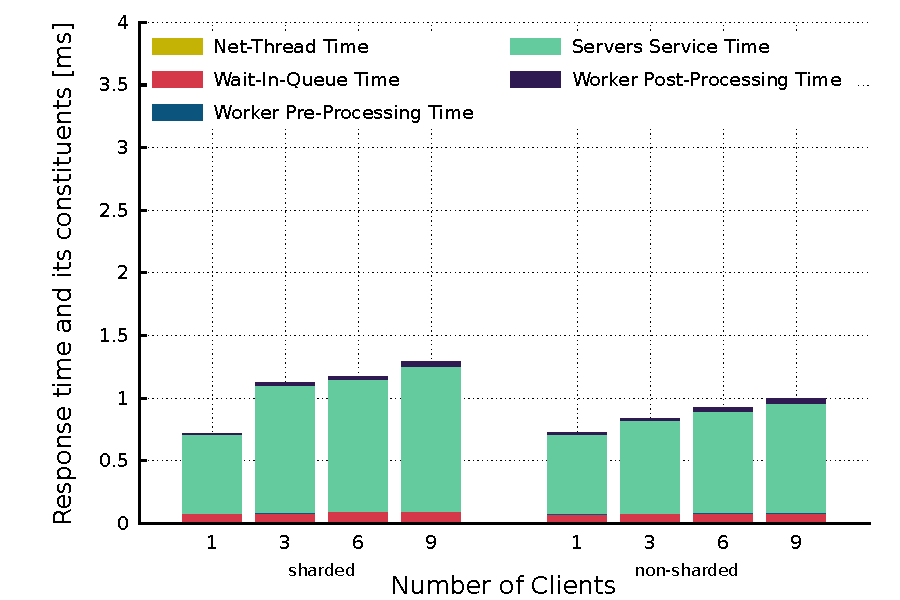
\includegraphics[width=0.5\linewidth]{../plots/experiment_gets/timers_2/ALL_TIMES_TOGETHER.pdf}
	\caption{\textit{Experiment with GETs and multi-GETs.} Break-down of response time (as measured on the middleware) into it's constituents vs number of keys in both, sharded and non-sharded case. Error bars are omitted for clearance.}
	\label{Figure:experiment_gets_break-down}	
\end{figure}

\subsection{Non-sharded Case}

All parameters remain the same, only sharding is disabled on the middleware.

\subsubsection{Explanation}

As sharding is now disabled, request is not replicated at the middleware, which should save processing time, but one message in the network is of approximate length 1KB, 3KB, 6KB and 9kB, for 1, 3, 6 and 9 keys respectively. Response time (Figure \ref{Figure:experiment_gets:a}) is increasing with increase in number of keys because of this, yet on average, even request with 9 keys is processed in around 2ms.

We observe similar behavior in percentile plot (Figure \ref{Figure:experiment_gets_all:a}): individual percentiles are increasing with increase in number of keys, slightly for 25\textsuperscript{th}, 50\textsuperscript{th} and 75\textsuperscript{th} percentiles, but more significantly for 90\textsuperscript{th} and 99\textsuperscript{th} percentiles. This is again consequence of longer messages and is further discussed in subsection "Histogram". Finally, values for GET requests with 1 key are the same here as in previous subsection, since in both cases sharding does not occur.

From Figure \ref{Figure:experiment_gets_break-down}, conclusion is that system is not saturated with current (\#clients, \#workers) configuration since waiting-in-queue times are very low. The bottleneck of this setup is after the middleware (servers and network between middlewares and servers).

\subsection{Histogram}

Histograms from Figure \ref{Figure:histograms} display density distribution of requests with 6 keys over response time duration. They are plotted with bucket size of 0.1ms and in range [0, 10 ]ms they display on average around 99.5\% of all requests.

Generally, for both sharded and non-sharded case, majority of requests are concentrated below 2ms. Furthermore, histograms at middleware seem to be "closer to 0" than histograms at clients. This is because of additional travel times between middleware and memtier. Also, histograms at middleware are "more narrow" (more concentrated) than histograms at clients. I believe this is due to responses traveling between middleware and clients, where network adds some additional latency that varies from message to message. When comparing histograms at client for sharded and non-sharded case (Figures \ref{Figure:histograms:a} and \ref{Figure:histograms:b}), we can observe that histogram in non-sharded case is more concentrated ("more narrow") and closer to 0 than in sharded case. This complies with response times (Figure \ref{Figure:experiment_gets}) that are higher for sharded case. Reasons for this are discussed below.

Histogram plots conform with percentile plots in Figure \ref{Figure:experiment_gets_all}: around 75\% of requests are processed in around 2ms, 90\% of requests are processed in around 6ms, and 99\% of requests are processed in around 9ms - 9\% of requests have response times between 6 and 9ms and they are visible as small "hill" around 8ms point in histograms. It is difficult to claim the reason for this, but since each worker has processed no more than 4000 requests, this is not due to logging (reminder, logging takes place only after 20000 processed requests, or in the end from shut-down thread). Most probably it is due to the network fluctuations: request travels 4 times, twice between client and middleware and twice between middleware and servers, and packets could be delayed on some of these sections. This delay (if happens between middleware and server) can prolong server-service-time at the middleware since it must wait for all responses from all servers to assemble them. In non-sharded case where assembling takes no place, messages are longer and are not sent in one packet, so middleware still needs to wait to collect full response. Furthermore, this "hill" is lower and concentrated around 7.5ms point when measured on the middleware, but is higher and concentrated around 8ms point when measured on the client. Since there is only network between client and middleware, this is another proof that network latencies are responsible for this discrepancy. As for why this is not random, but concentrated around 8ms, I have no explanation, but it's not because of middleware. From histogram of server service time (Figure \ref{Figure:histograms_sst}), this discrepancy comes from after the middleware, and netowrk and middleware just add on top of it.

\begin{figure}[ht!]
	\centering	
	\subfloat[non-sharded case at client]{%
		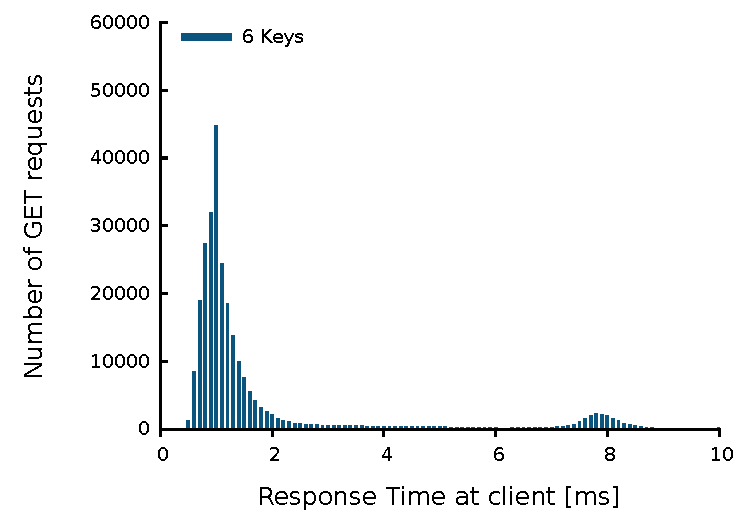
\includegraphics[width=0.49\linewidth]{../plots/experiment_gets/HISTOGRAM_MT_6KEYS_NONSHARDED.pdf}
		\label{Figure:histograms:a}}\hfill
	\subfloat[sharded case at client]{%
		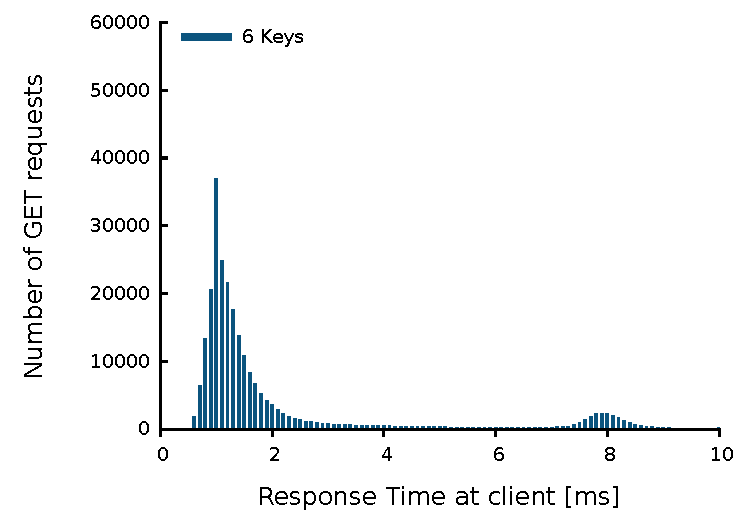
\includegraphics[width=0.49\linewidth]{../plots/experiment_gets/HISTOGRAM_MT_6KEYS_SHARDED.pdf}
		\label{Figure:histograms:b}}\\
	\subfloat[non-sharded case at middleware]{%
		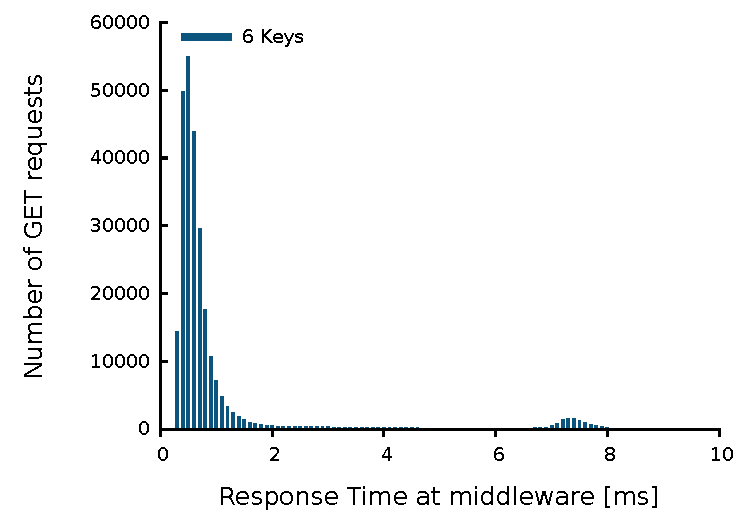
\includegraphics[width=0.49\linewidth]{../plots/experiment_gets/HISTOGRAM_MW_6KEYS_NONSHARDED.pdf}
		\label{Figure:histograms:c}}\hfill
	\subfloat[sharded case at middleware]{%
		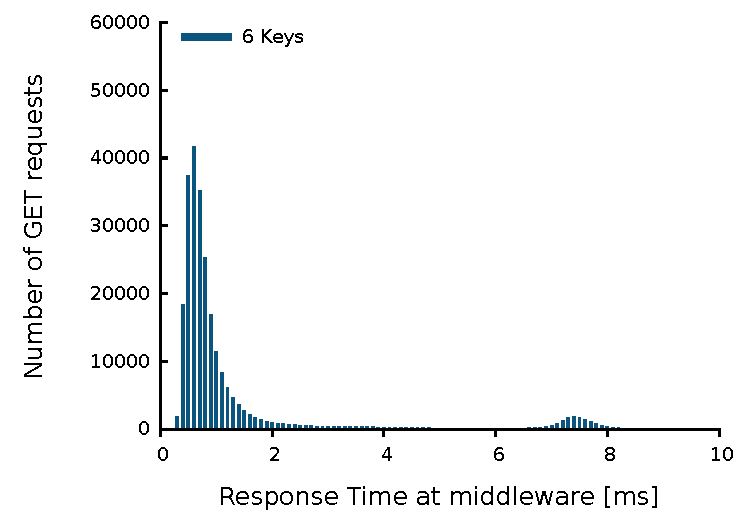
\includegraphics[width=0.49\linewidth]{../plots/experiment_gets/HISTOGRAM_MW_6KEYS_SHARDED.pdf}
		\label{Figure:histograms:d}}\\
	\caption{\textit{Experiment with GETs and multi-GETs.} Histograms of response time for requests with 6 keys as measured on the client and on the middleware, in both, sharded and non-sharded case.}
	\label{Figure:histograms}	
\end{figure}

\begin{figure}[ht!]
	\centering	
	\subfloat[non-sharded case]{%
		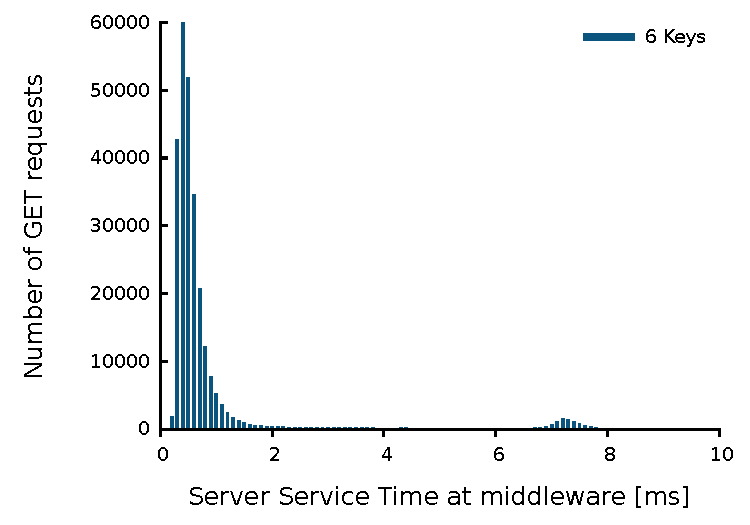
\includegraphics[width=0.49\linewidth]{../plots/experiment_gets/HISTOGRAM_MW_6KEYS_NONSHARDED_SST.pdf}
		\label{Figure:histograms_sst:a}}\hfill
	\subfloat[sharded case]{%
		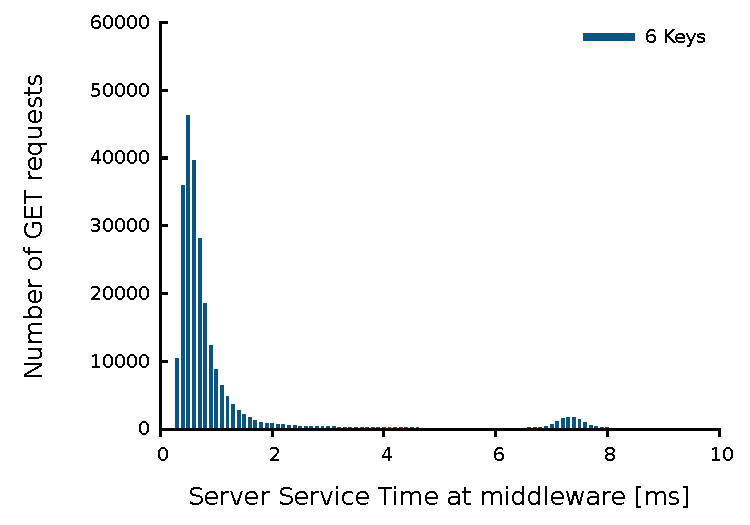
\includegraphics[width=0.49\linewidth]{../plots/experiment_gets/HISTOGRAM_MW_6KEYS_SHARDED_SST.pdf}
		\label{Figure:histograms_sst:b}}\\
	\caption{\textit{Experiment with GETs and multi-GETs.} Histograms of server service time for requests with 6 keys in both, sharded and non-sharded case.}
	\label{Figure:histograms_sst}	
\end{figure}

\subsection{Summary}

Response times are lower in non-sharded case and also corresponding percentiles are lower. Even though first assumption may be that it takes longer for server to process more keys (9 in non-sharded case compared to 3 in sharded case for example), this is not dominant factor in this setup. Sending 3 messages (to 3 servers) and waiting for 3 responses takes longer time because of network latency. Hence, for multiple keys, it is (on average) faster to disable sharding. However, the difference is not very large - less than 0.5ms. 

In both cases, 75\% of requests are processed in around 2ms and 99\% in under 10ms. The discrepancy ("the hill") is present with sharding enabled and disabled and for all keys\footnote{Histogram plots for other keys are available in the repository.}.

%%%%%%%%%%%%%%%%%%%%%%%%%%%%%%%%%%%%%%%%%%%%%%%%%%%%%%%%%%%%%%%%%%%%%%%%%%%%%%%%%%%%%%%%%%%%%%%%%%%%%%%%%
%%%%%%%%%%%%%%%%%%%%%%%%%%%%%%%%%%%%%%%%%%%%%%%%%%%%%%%%%%%%%%%%%%%%%%%%%%%%%%%%%%%%%%%%%%%%%%%%%%%%%%%%%
%%%%%%%%%%%%%%%%%%%%%%%%%%%%%%%  2K ANALYSIS
%%%%%%%%%%%%%%%%%%%%%%%%%%%%%%%%%%%%%%%%%%%%%%%%%%%%%%%%%%%%%%%%%%%%%%%%%%%%%%%%%%%%%%%%%%%%%%%%%%%%%%%%%
%%%%%%%%%%%%%%%%%%%%%%%%%%%%%%%%%%%%%%%%%%%%%%%%%%%%%%%%%%%%%%%%%%%%%%%%%%%%%%%%%%%%%%%%%%%%%%%%%%%%%%%%%

\section{2K Analysis (90 pts)}

In this section results from 2k analysis are presented. Individual parameters used in this section are listed in table \ref{table:2k:params}. All experiments in this section are run on the same set of physical machines. The results are calculated using "sign table" method, where $-1$ corresponds to lower level and $+1$ to higher level of 3 variable factors - Number of memcached servers (\textbf{MC}), number of middlewares (\textbf{MW}) and number of workers per middleware (\textbf{WC}). This is listed in table \ref{table:2k:symbols}.

\begin{center}
	\scriptsize{	
		\begin{table}[!ht]
			\centering
			\begin{tabulary}{\linewidth}{ | L | C |}
				\hline Number of servers	&	2 and 3	\\
				\hline Number of client machines	&	3	\\
				\hline Instances of memtier per machine	&	2	\\
				\hline Threads per memtier instance	&	1	\\
				\hline Virtual clients per thread	&	32	\\
				\hline Workload	&	Write-only, Read-only and 50-50-read-write	\\
				\hline Number of middlewares	&	1 and 2	\\
				\hline Worker threads per middleware	&	8 and 32	\\
				\hline 
			\end{tabulary}
			\caption{\textit{Individual parameters for 2k analysis experiments.}}
			\label{table:2k:params}
		\end{table}
	}
\end{center}

\begin{center}
	\scriptsize{	
		\begin{table}[!ht]
			\centering
			\begin{tabulary}{\linewidth}{ | C | C | C | C | }
				\hline 	&	Number of servers (\textbf{MC})	&	Number of middlewares (\textbf{MW})	& Number of workers (\textbf{WC})	\\
				\hline	-1	&	2	&	1	&	8	\\
				\hline	1	&	3	&	2	&	32	\\
				\hline 
			\end{tabulary}
			\caption{\textit{2k Analysis.} Correspondence between values in sing table and parameter levels.}
			\label{table:2k:symbols}
		\end{table}
	}
\end{center}

Input to 2k Analysis is throughput and response time in each repetition of expriments under varying configuration. Output of the analysis is the effect each of factors has on overall performance. Additive model was used to perform this analysis. Results are presented in tables \ref{table:2k:read-only}, \ref{table:2k:write-only} and \ref{table:2k:50-50} where: MC-MW illustrates joint effect of number of servers and middlewares and so on, and finally MC-MW-WC illustrates joint effect of varying number of servers, middlewares and workers per middleware. Column "Effects" showcases effects values ($q$-values in "sign table" notation), column "Variation" displays what percent of variation is explained by each of the effects, and finally in column "Confidence Interval", 90\% confidence interval is displayed for each of the effects. Note that "mean" is mean of all values from all repetitions and configurations, hence has no variation percentage. "Error" is error due to repetitions and has no effect value nor can have estimate of confidence interval. Confidence interval with * are not significant since they include 0. Due to rounding, values that are smaller than $10^{-3}$ appear as just $0.00$.
	
\begin{table}[!ht]
	\begin{adjustbox}{center}
		\begin{tabulary}{\linewidth}{ C | C | C | C | c | C | C | }
			\cline{2-7}	&	\multicolumn{3}{| c |}{\textbf{Throughput}}	&	\multicolumn{3}{| c |}{\textbf{Response Time}}	\\
			\cline{2-7} &	Effects	&	Variation [\%]	&	Confidence Interval	&	Effects	&	Variation [\%]	&	Confidence Interval	\\
			\hline	\multicolumn{1}{| c |}{mean}	&	10877.34	&	-		&	(10748.8, 11005.8)	&	22.66	&	-	& (21.9, 23.4)
			\\
			\hline	\multicolumn{1}{| c |}{MC}	&	-291.13	&	0.24	&	(-419.6, -162.6)	&	0.04	&	0.0	&	(-0.7, 0.8)*	\\
			\hline	\multicolumn{1}{| c |}{MW}	&	3772.56	&	\textbf{40.66}	&	(3644.1, 3901.1)	&	-7.54	&	\textbf{42.23}	&	(-8.3, -6.8)	\\
			\hline	\multicolumn{1}{| c |}{WC}	&	4242.75	&	\textbf{51.43}	&	(4114.3,  4371.2)	&	-8.28	&	\textbf{50.9}	&	(-9.0, -7.5)	\\
			\hline	\multicolumn{1}{| c |}{MC-MW}	&	-119.54	&	0.04	&	(-248.0, 8.9)*	&	-0.004	&	0.0	&	(-0.7, 0.7)*	\\
			\hline	\multicolumn{1}{| c |}{MC-WC}	&	41.42	&	0.005	&	(-87.1, 169.2)*	&	-0.02	&	0.0	&	(-0.8, 0.7)*	\\
			\hline	\multicolumn{1}{| c |}{MW-WC}	&	1606.25	&	\textbf{7.37}	&	(1477.8, 	1734.7)	&	2.51	&	\textbf{4.7}	&	(1.8, 3.3)	\\
			\hline	\multicolumn{1}{| c |}{MC-MW-WC}	&	-23.72	&	0.00	&	(-152.2, 104.8)*	&	0.14	&	0.01	&	(-0.6, 0.9)*	\\
			\hline	\multicolumn{1}{| c |}{Error}	&	-	&	0.25	&	-	&	-	&	2.2	&	-	\\
			\hline 
		\end{tabulary}
	\end{adjustbox}		
	\caption{\textit{2k Analysis.} Results under read-only load. Confidence intervals with * are not significant.}
	\label{table:2k:read-only}
\end{table}

\textbf{\textit{Read-Only load.}} In all previous experiments with read-only load, the bottleneck was server's maximal outbound bandwidth that fixed throughput, and we were not able to notice the influence of varying number of workers and middlewares. Here, however, 2 servers can theoretically send maximum of 24 MB/s which is also theoretical maximum for outbound traffic of one client machine. Now that bottleneck is not on servers' side, influence of these factors is observed and discussed.

Analysis shows(table \ref{table:2k:read-only}) that for both throughput and response time, most variation is explained by varying number of workers (51.43\% and 50.9\%, respectively) and varying number of middlewares (40.66\% and 42.23\%, respectively). Mixed effect of these two factors explains 7.37\% and 4.7\% of variation, which is significantly lower than their individual effect, but still more significant then any other effect. From the sign of effects we can conclude that increasing number of middlewares and workers per middleware increases throughput ("+" sign in corresponding "Effects" cells), and decreases response time ("-" sign in corresponding "Effects" cells). Interestingly, effect of varying number of servers is very low for throughput (only 0.21\%), but for response time it's insignificant (confidence interval contains 0). Since all GET requests contain only 1 key, requests are forwarded to only one chosen server, and with bottleneck lifted from servers' side, having 2 or 3 servers does not make a difference. High percentages of variation explained by number of middlewares and workers show that bottleneck in this setup is middleware since increasing either number of middlewares, worker threads or both, improves performance.

The remaining combination of effects are insignificant. Error, however, explains variation in higher percentage than number of servers, both for throughput and response time. This most probably comes from network latencies.

	
\begin{table}[!ht]
	\begin{adjustbox}{center}
		\begin{tabulary}{\linewidth}{ C | C | C | C | c | C | C | }
			\cline{2-7}	&	\multicolumn{3}{| c |}{\textbf{Throughput}}	&	\multicolumn{3}{| c |}{\textbf{Response Time}}	\\
			\cline{2-7} &	Effects	&	Variation [\%]	&	Confidence Interval	&	Effects	&	Variation [\%]	&	Confidence Interval	\\
			\hline	\multicolumn{1}{| c |}{mean}	&	7582.66	&	-		&	(7324.5, 7840.8)	&	31.74	&	-	&	(31.0, 32.5)	\\
			\hline	\multicolumn{1}{| c |}{MC}	&	-6.53	&	0.00	&	(-264.7, 251.6)*	&	-0.02	&	0.00	&	(-0.8, 0.7)*	\\
			\hline	\multicolumn{1}{| c |}{MW}	&	2333.0	&	\textbf{39.82}	&	(2074.8, 2591.2)	&	-9.47	&	\textbf{40.5}	&	(-10.2, -8.7)	\\
			\hline	\multicolumn{1}{| c |}{WC}	&	2659.02	&	\textbf{51.72}	&	(2400.9, 2917.2)	&	-10.97	&	\textbf{54.34}	&	(-11.7, -10.2)	\\
			\hline	\multicolumn{1}{| c |}{MC-MW}	&	31.66	&	0.01	&	(-226.5, 289.8)*	&	0.006	&	0.00	&	(-0.7, 0.8)*	\\
			\hline	\multicolumn{1}{| c |}{MW-WC}	&	-7.25	&	0.00	&	(-265.4, 250.9)*	&	0.14	&	0.01	&	(-0.6, 0.9)*	\\
			\hline	\multicolumn{1}{| c |}{MW-WC}	&	895.99	&	\textbf{5.87}	&	(637.8, 1154.2)	&	2.89	&	\textbf{3.76}	&	(2.1, 3.6)	\\
			\hline	\multicolumn{1}{| c |}{MC-MW-WC}	&	57.52	&	0.02	&	(-200.6, 315.7)*	&	-0.26	&	0.03	&	(-1.0, 0.5)*	\\
			\hline	\multicolumn{1}{| c |}{Error}	&	-	&	2.56	&	-	&	-	&	1.36	&	-	\\
			\hline 
		\end{tabulary}
	\end{adjustbox}	
	\caption{\textit{2k Analysis.} Results under write-only load. Confidence intervals with * are not significant.}
	\label{table:2k:write-only}
\end{table}


\textbf{\textit{Write-Only load.}} In previous experiments the bottleneck was always in middleware(s), and we have already observed that increasing number of workers improves throughput and lowers response time (Figure \ref{Figure:baseline_1midd:b} and \ref{Figure:baseline_1midd:d} for 1 middleware and 1 server and Figures \ref{Figure:baseline_2midd_2vms:a} and \ref{Figure:baseline_2midd_2vms:b} with 2 middlewares and 1 server and Figures \ref{Figure:experiment_write-only:a} and \ref{Figure:experiment_write-only:b} with 2 middlewares and 3 servers).

This is verified with 2k Analysis results in table \ref{table:2k:write-only}. For both, throughput and response time, most variation is explained by varying number of workers (51.72\% and 54.34\%, respectively) and varying number of middlewares (39.82\% and 40.5\% respectively). According to the sign of corresponding "Effects" value, increasing these factors results in increased throughput and decreased response time, as was already observed based on previous experiments. This confirms again that the bottleneck in this setup is at middleware (number of them and number of workers per middleware). Joint effect of these 2 factors are not as influential (6.05\% for throughput and 3.6\% for response time), but are more significant than any other. However, with increasing number of middlewares and number of workers per middleware together (MW-WC), both throughput and response time are increased.

The rest of effects are statistically insignificant, including varying number of servers. In write-only load, servers' side was never bottleneck, so it was expected that increasing number of servers will make no difference. Note that with increasing number of servers, SET requests must be replicated and sent to all available servers, so it was fair to assume that increase of servers count will make more significant difference - to decrease throughput and increase response time. However, effects of sending one additional SET request (between having 2 and 3 servers) contributes much less than number of workers. Moreover, even error explains higher percentage of variation than number of servers - 2.56\% and 1.36\% for throughput and response time respectively. These can again be contributed to network latency.
	
\begin{table}[!ht]
	\begin{adjustbox}{center}
		\begin{tabulary}{\linewidth}{ C | C | C | C | c | C | C | }
			\cline{2-7}	&	\multicolumn{3}{| c |}{\textbf{Throughput}}	&	\multicolumn{3}{| c |}{\textbf{Response Time}}	\\
			\cline{2-7} &	Effects	&	Variation [\%]	&	Confidence Interval	&	Effects	&	Variation [\%]	&	Confidence Interval	\\
			\hline	\multicolumn{1}{| c |}{mean}	&	9203.53	&	-	&	(8984.1, 9422.9)	&	26.05	&	-	&	(25.0, 27.1)	\\
			\hline	\multicolumn{1}{| c |}{MC}	&	9.61	&	0.00	&	(-209.8, 229.0)*	&	-0.17	&	0.02	&	(-1.2, 0.9)*	\\
			\hline	\multicolumn{1}{| c |}{MW}	&	2924.87	&	\textbf{43.7}	&	(2705.5, 3144.3)	&	-8.03	&	\textbf{43.23}	&	(-9.1, -7.0)	\\
			\hline	\multicolumn{1}{| c |}{WC}	&	3094.99	&	\textbf{48.93}	&	(2875.6, 3314.4)	&	-8.58	&	\textbf{49.36}	&	(-9.6, -7.5)	\\
			\hline	\multicolumn{1}{| c |}{MC-MW}	&	-73.58	&	0.03	&	(-293.0, 145.8)*	&	0.24	&	0.04	&	(-0.8, 1.3)*	\\
			\hline	\multicolumn{1}{| c |}{MC-WC}	&	-3.4	&	0.00	&	(-222.8, 216.0)*	&	0.03	&	0.00	&	(-1.0, 1.1)*	\\
			\hline	\multicolumn{1}{| c |}{MW-WC}	&	1088.28	&	\textbf{6.05}	&	(868.9, 1307.7)	&	2.32	&	\textbf{3.6}	&	(1.3, 3.3)	\\
			\hline	\multicolumn{1}{| c |}{MC-MW-WC}	&	-41.37	&	0.01	&	(-260.8, 178.0)*	&	-0.03	&	0.00	&	(-1.1, 1.0)*	\\
			\hline	\multicolumn{1}{| c |}{Error}	&	-	&	1.29	&	-	&	-	&	\textbf{3.75}	&	-	\\
			\hline 
		\end{tabulary}
	\end{adjustbox}	
	\caption{\textit{2k Analysis.} Results under 50-50-write-read load. Confidence intervals with * are not significant.}
	\label{table:2k:50-50}
\end{table}

\textbf{\textit{50-50-read-write load.}} Even under mixed load, 2k Analysis gives similar results: for both, throughput and response time, most of variation is explained by number of workers (48.93\% and 49.36\%, respectively) and number of middlewares (43.7\% and 43.23\%, respectively). From the sign of corresponding "Effects" values, increasing these 2 factors will increase throughput and decrease response time, which complies with results obtained under read-only and write-only load. Mixture of these 2 factors is less influential (6.05\% and 3.6\% for throughput and response time, respectively), but still more significant than any other effect. Increasing both these factors simultaneously results in increased throughput and response time. All of this implies that bottleneck under mixed load is at middleware(s).

The rest of the factors and their mixtures are insignificant. Again, increasing number of servers makes no difference, which conforms with findings obtained under read-only and write-only load. More variation is explained by errors than by number of servers - 1.29\% for throughput and 3.75\% for response time. Furthermore, percentage explained by errors for response time is the highest recorded, and is higher than influence of mixed effects of number of workers and number of middlewares. The reason for this, I believe, is due to the fact that response times for write-only is higher than for read-only load. In case of read-only load, mean response time over all configurations and repetitions is  22.66ms, but in case of write-only load it is 31.74ms.


%%%%%%%%%%%%%%%%%%%%%%%%%%%%%%%%%%%%%%%%%%%%%%%%%%%%%%%%%%%%%%%%%%%%%%%%%%%%%%%%%%%%%%%%%%%%%%%%%%%%%%%%%
%%%%%%%%%%%%%%%%%%%%%%%%%%%%%%%%%%%%%%%%%%%%%%%%%%%%%%%%%%%%%%%%%%%%%%%%%%%%%%%%%%%%%%%%%%%%%%%%%%%%%%%%%
%%%%%%%%%%%%%%%%%%%%%%%%%%%%%%%  QUEUEING THEORY
%%%%%%%%%%%%%%%%%%%%%%%%%%%%%%%%%%%%%%%%%%%%%%%%%%%%%%%%%%%%%%%%%%%%%%%%%%%%%%%%%%%%%%%%%%%%%%%%%%%%%%%%%
%%%%%%%%%%%%%%%%%%%%%%%%%%%%%%%%%%%%%%%%%%%%%%%%%%%%%%%%%%%%%%%%%%%%%%%%%%%%%%%%%%%%%%%%%%%%%%%%%%%%%%%%%


\section{Queuing Model (90 pts)}

This section focuses on modeling and mathematical formulation of the system. First, we start off with the simplest model and moving on to more complex ones. Input values to the model(s) are used from already conducted experiments. The following notation is used for first 2 models:
\begin{itemize}
	\item $\lambda$ is arrival rate, calculated as $1/\mathbb{E}[\tau]$, where $\tau$ is interarrival time - time between arrivals (to middleware) of 2 consecutive requests, and $\mathbb{E}[\tau]$ is mean interarrival time. These values are obtained directly from middleware logs.
	\item $\mu$ is service rate. True service rate value is difficult to obtain, but here we are using the best estimate we can - the highest service rate observed under configuration that gives the highest throughput. Service rate of each worker is calculated as $1/\mathbb{E}[s]$ where $s$ is service time of a worker thread - time between dequeuing from internal request queue until sending final response to the client, and $\mathbb{E}[s]$ is mean value of all service times of all requests processed by worker. The highest service rate obtained this way is used in further calculations.
	\item $\rho$ is traffic intensity and is calculated differently, depending on a model.
	\item $p_0$ and $p_q$ is probability of having zero jobs in the system, and queueing probability (with m services, probability of at least m jobs in the system), respectively
	\item $U$ is component utilization
	\item $\mathbb{E}[n]$, $\mathbb{E}[n_q]$ and $\mathbb{E}[n_s]$ are expected number of jobs in the system, in the queue and in service, respectively
	\item $\mathbb{E}[r]$ and $\mathbb{E}[w]$ are expected response time and time spent waiting in the queue, respectively
\end{itemize} 

\subsection{M/M/1}

In this section, the system we are modeling is from Section 4 with 3 client machines, 2 middlewares and 3 servers, each middleware having 8, 16, 32 or 64 worker threads. $M/M/1$ models the system as one queue and one service where jobs arrive by rate $\lambda$ and the service services one request at a time with speed $\mu$. These 2 values are input to the system. Service rate $\mu$ is extracted from configuration that gave the highest throughput in these experiments: 30 clients for 8 workers, 312 clients for 16 workers and 384 clients for 32 and 64 workers, and arrival rate $\lambda$ corresponds to 192-client load. Given that we have 2 middlewares, total number of workers is 16, 32, 64 and 128 for 8, 16, 32 and 64 worker configuration, respectively. Since in this model we have only 1 service, its service rate is total service rate of all workers in both middlewares, hence $m\cdot\mu$ where $m$ is total number of workers and $\mu$ is highest service rate per worker (in the table \ref{table:MM1}, $m\cdot\mu$ value is displayed). 

Results are displayed in table \ref{table:MM1}. Input values are only measured (and not predicted) and some of the parameters are not measured on the middleware (like $p_0$ and $U$), for the rest both values are displayed. Although equal number of clients are generating load, we consider systems with different number of workers as separate individual systems. This is why arrival rate and service rate are different for different worker configurations.

Utilization is decreasing as number of workers increases, and that matches our findings from Section 4 - 8 workers are more busy resulting in higher queue size, while 64 workers with the same load are less busy and have lower queue size. Note that service time of this one service includes servers-service time as well, and component utilization cannot differentiate between the two, but utilization percentages are very high matching to our findings that bottleneck is in middleware (but model is not correct for our setup as will be discussed later in the paragraph). Probability of having 0 jobs in the system $p_0$ are, in my opinion, over-estimated, but it is increasing as number of workers increases which was expected as more workers are faster, hence queue size is shorter. Mean number of jobs in the system, in the queue and in the service are very under-estimated. As $M/M/1$ models only 1 service and service can process only 1 job at the time, values for $\mathbb{E}[n_s]$ between 0.93 and 0.81 seem reasonable, indicating that only 1 job can indeed be processed at the time. Because of this, total number of jobs in the system and number of jobs waiting in the queue differ by around 1. This is first indicator that the model gives correct results with given input values, but is just not correct model of our system. Mean response times and mean times spent in the queue are also very under-estimated. 

Note that the best estimate for service rate is used in these calculations which is over-estimation by itself comparing to real-world measured values, and can lead to "too good" results. However, the model itself does not correspond to actual setup: there are multiple threads working in parallel, while in $M/M/1$ there is only 1 service; there are 2 internal request queues in actual setup, but in the model there is only 1, and these are the reasons behind very large differences between predicted and measured values.
	
\begin{table}[!ht]
	\begin{adjustbox}{center}
		\begin{tabulary}{\linewidth}{ C | C | C | C | c | C | C | C | C | }
			\cline{2-9}	&	\multicolumn{2}{| c |}{\textbf{WORKERS = 8}}	&	\multicolumn{2}{| c |}{\textbf{WORKERS = 16}}	&	\multicolumn{2}{| c |}{\textbf{WORKERS = 32}}	&	\multicolumn{2}{| c |}{\textbf{WORKERS = 64}}	\\
			\cline{2-9} &	predicted	&	measured	&	predicted	&	measured	&	predicted	&	measured	&	predicted	&	measured	\\
			\hline	\multicolumn{1}{| c |}{$\lambda$ [req/s]}	&	-	&	7166.93	&	-	&	10126.99	&	-	&	11950.1	&	-	&	14098.71	\\
			\hline	\multicolumn{1}{| c |}{$\mu$ [req/s]}	&	-	&	7712.73	&	-	&	11875.77	&	-	&	13677.9	&	-	&	17387.41	\\
			\hline	\multicolumn{1}{| c |}{$\rho$}	&	0.93	&	-	&	0.85	&	-	&	0.87	&	-	&	0.81	&	-	\\
			\hline	\multicolumn{1}{| c |}{$p_0$ [\%]}	&	7.08	&	-	&	14.73	&	-	&	12.63	&	-	&	18.91	&	-	\\
			\hline	\multicolumn{1}{| c |}{$U$ [\%]}	&	92.92	&	-	&	85.27	&	-	&	87.37	&	-	&	81.09	&	-	\\
			\hline	\multicolumn{1}{| c |}{$\mathbb{E}[n]$}	&	13.13	&	99.44	&	5.79	&	102.57	&	6.92	&	106.75	&	4.29	&	139.15	\\
			\hline	\multicolumn{1}{| c |}{$\mathbb{E}[n_q]$}	&	12.2	&	83.44	&	4.94	&	70.57	&	6.04	&	42.75	&	3.48	&	11.15	\\
			\hline	\multicolumn{1}{| c |}{$\mathbb{E}[n_s]$}	&	0.93	&	16	&	0.85	&	32	&	0.87	&	64	&	0.81	&	128	\\
			\hline	\multicolumn{1}{| c |}{$\mathbb{E}[r]$ [ms]}	&	1.83	&	24.96	&	0.57	&	14.72	&	0.58	&	11.24	&	0.30	&	8.42	\\
			\hline	\multicolumn{1}{| c |}{$\mathbb{E}[w]$ [ms]}	&	0.002	&	22.81	&	0.0005	&	12.07	&	0.0005	&	6.77	&	0.0002	&	1.50	\\
			\hline 
		\end{tabulary}
	\end{adjustbox}	
	\caption{\textit{Queueing Models.} Predicted and measured parameters of M/M/1 model for all worker configurations under 192-clients load.}
	\label{table:MM1}
\end{table}


\subsection{M/M/m}

In this section we try to improve previous model by adding more services. Experiment setup remains the same, and instead of modeling the system as $M/M/1$ we model it as $M/M/16$, $M/M/32$, $M/M/64$ and $M/M/128$ for 8, 16, 32 and 64 workers per middleware, respectively. Worker service rate $\mu$ is calculated as before (and in table \ref{table:MMm} only $\mu$ is displayed), and $\lambda$ is calculated again for 192-client load. Results for all 4 worker configurations are displayed in table \ref{table:MMm}.

\begin{table}[!ht]
	\begin{adjustbox}{center}
		\begin{tabulary}{\linewidth}{ C | C | C | C | c | C | C | C | C | }
			\cline{2-9}	&	\multicolumn{2}{| c |}{\textbf{WORKERS = 8}}	&	\multicolumn{2}{| c |}{\textbf{WORKERS = 16}}	&	\multicolumn{2}{| c |}{\textbf{WORKERS = 32}}	&	\multicolumn{2}{| c |}{\textbf{WORKERS = 64}}	\\
			\cline{2-9} &	predicted	&	measured	&	predicted	&	measured	&	predicted	&	measured	&	predicted	&	measured	\\
			\hline	\multicolumn{1}{| c |}{$\lambda$ [req/s]}	&	-	&	7166.93	&	-	&	10126.99	&	-	&	11950.1	&	-	&	14098.71	\\
			\hline	\multicolumn{1}{| c |}{$\mu$ [req/s]}	&	-	&	482.05	&	-	&	371.12	&	-	&	213.72	&	-	&	135.84	\\
			\hline	\multicolumn{1}{| c |}{$\rho$}	&	0.93	&	-	&	0.85	&	-	&	0.87	&	-	&	0.81	&	-	\\
			\hline	\multicolumn{1}{| c |}{$p_q$}	&	0.7	&	-	&	0.29	&	-	&	0.21	&	-	&	0.01	&	-	\\
			\hline	\multicolumn{1}{| c |}{$U$ [\%]}	&	92.92	&	-	&	85.27	&	-	&	87.37	&	-	&	81.09	&	-	\\
			\hline	\multicolumn{1}{| c |}{$\mathbb{E}[n]$}	&	24.03	&	99.44	&	28.97	&	102.57	&	57.37	&	106.75	&	103.85	&	139.15	\\
			\hline	\multicolumn{1}{| c |}{$\mathbb{E}[n_q]$}	&	9.16	&	83.44	&	1.68	&	70.57	&	1.46	&	42.75	&	0.06	&	11.15	\\
			\hline	\multicolumn{1}{| c |}{$\mathbb{E}[n_s]$}	&	14.87	&	16	&	27.29	&	32	&	55.91	&	64	&	103.79	&	128	\\
			\hline	\multicolumn{1}{| c |}{$\mathbb{E}[r]$ [ms]}	&	3.35	&	24.96	&	2.86	&	14.72	&	4.8	&	11.24	&	7.37	&	8.42	\\
			\hline	\multicolumn{1}{| c |}{$\mathbb{E}[w]$ [ms]}	&	1.28	&	22.81	&	0.17	&	12.07	&	0.12	&	6.77	&	0.004	&	1.50	\\
			\hline 
		\end{tabulary}
	\end{adjustbox}	
	\caption{\textit{Queueing Models.} Predicted and measured parameters of M/M/m model for all 4 worker configurations under 192-clients load.}
	\label{table:MMm}
\end{table}

Even though, theoretically, service rate of individual service should be constant and independent of load and external factors, this is just best-effort estimation, and systems with varying number of workers with same physical resources (CPU, RAM..) are considered different independent systems. Hence, service rate per worker varies with number of workers. Arrival rates are the same as in previous subsection, and so is traffic intensity $\rho$.

Average utilization $U$ per service remains the same and are decreasing as number of worker increases, which was expected for the reasons mentioned above. These percentages are now per service, which matches our findings that the bottleneck is insufficient number of workers (even though service time per worker here includes servers-service time as well). Probability that there are at least $m$ jobs in the system ($m$ is number of services), $p_q$, is displayed in the table instead of $p_0$ since it is essential for further results. We can observe that for 8-workers-per-middleware configuration this probability is very high, and given that there are 192 clients (and theoretically maximum 192 jobs in the whole system) and only 16 services, it is very likely that there are at least 16 jobs in the system. However, for 64 worker configuration, this probability is very small, and, I believe, under-estimated. 

Measured values reported in table \ref{table:MMm} for number of jobs in the queue correspond to average queue length over \textit{both} queues in 2 middlewares, which means that twice as many jobs are actually waiting in parallel in the system. Measured number of jobs currently under service equals to number of worker threads $m$, and measured total number of jobs in the system equals to $m + queue size$. Predicted mean number of jobs in the system, in the queue and in the service are again under-estimated, but are better predictions than in $M/M/1$ model. Predictions for $\mathbb{E}[n_s]$ are very good, and they are very close to the total number of services in the system ($m$) where each of them can process only 1 job at the time. Estimates for mean number of jobs in the queue are still under-estimated. Overall, prediction for total number of jobs in the system is also under-estimated, but for 64 worker configuration it gets the closest to measured value, with difference that all of them are being currently processed, whereas real situation shows that on average 11 jobs are waiting in the queue. 

Predictions for response times and times spent waiting in the queue are also under-estimated, but still better predictions compared to previous model. Predicted response time for 64 worker configuration is very close to measured value, but prediction for $\mathbb{E}[w]$ is not.

Although this model has improved some predictions, some other ones are still very under-estimated. The values used for service rate are again overly-optimistic - it is the fastest rate, and not all workers can have the same rate or even reach the fastest one, which can lead to under-estimation of some values, but, in my opinion, not this much. Having $m$ services in parallel did help, but there is still issue that we model only 1 queue and there are 2 queues in real setup.
	


\subsection{Network of Queues}

To overcome problems of models in previous subsections, we move to Network of Queues model. All network of queues are modeled as closed networks which implies that fixed number of jobs are circulating in the network. This perfectly fits actual implementation where client is blocked until it receives response from previous request, and only then generates another one, which means that number of jobs in the system at any time point is equal to number of clients.

All modeling in this subsection is based on Section 3, with 1 and 2 middlewares. Network is modeled as delay center (has infinitely many services, so queueing time is 0, but service time is not) since we just want to "slow-down" jobs, and not to enqueue them. Half of difference between response time as measured on the client and as measured on the middleware is taken as service time of network delay center ($(r_{client} - r_{mw})/2$). 

Client machine is modeled as delay-center as well. Service time of client delay-center is very small, and is often used to tune the system to avoid numerical instabilities \footnote{http://www.moreno.marzolla.name/software/queueing/queueing.html\#References  Chapter 5.2.2}.

Middleware is broken into 2 parts: net-thread modeled as $M/M/1$ because there is only 1 net-thread per middleware and requests are queued in \texttt{Selector} object of Net-Thread; and internal request queue with workers is modeled as $M/M/m$ where $m$ is number of workers. Service time of workers is calculated as the shortest service time observed (over all workers in all middlewares) in configuration that gives highest throughput.Net-thread service time is calculated in the same way (only among net-threads). Configuration with highest throughput is chosen since it should provide the best estimate of true service time.

Note that memcached server is not modeled. Assume that server is modeled as $M/M/1$ for example, and that all jobs departing from middleware are sent to server. From this follows that as soon as worker finishes with preprocessing phase and sends request to the server, it \textit{must} take another request, which would mean that 2 jobs are processed at the same time by the same worker-thread, which is contradiction to \textit{Single-Resource Possesion} necessary condition of product-form networks \footnote{Raj K. Jain - The Art of Computer Systems Performance Analysis, Chapter 32.2} (such as this one): "A job may not be present (waiting for service or receiving service) at two or more devices at the same time.". For this reason, time spent in traveling (2 times!) between middleware and server and server-processing time are included in service time of worker thread.

All models are implemented using \texttt{queueing}\footnote{http://www.moreno.marzolla.name/software/queueing/} package in Octave. Since closed networks and \texttt{qnsolve} method supports delay-centers only of form \texttt{"-/g/inf"}, this is actual model of network and client machine. The following notation (adopted from this package) is used:
\begin{itemize}
	\item $R$ is component response time. Here we are focusing on response time as measured on the middleware, $R_{mw}$.
	\item $X$ is total throughput in the system
	\item $Q$ is number of jobs in queue, per component. Here, we are focusing on queue size as measured on the middleware, $Q_{mw}$.
	\item $U$ is component utilization: $U_{mw}$ of middleware and $U_{nt}$ of net-thread.
\end{itemize}

\subsubsection{Network of Queues with 1 middleware}

Results of modeling system with 1 middleware are presented in this subsection. All input values are from baseline experiment with 1 middleware (Section 3.1) under read-only load and varying load and number of workers. Visualization of the network is given in figure \ref{Figure:noq_1midd}.

\begin{figure}[ht!]
	\centering		
	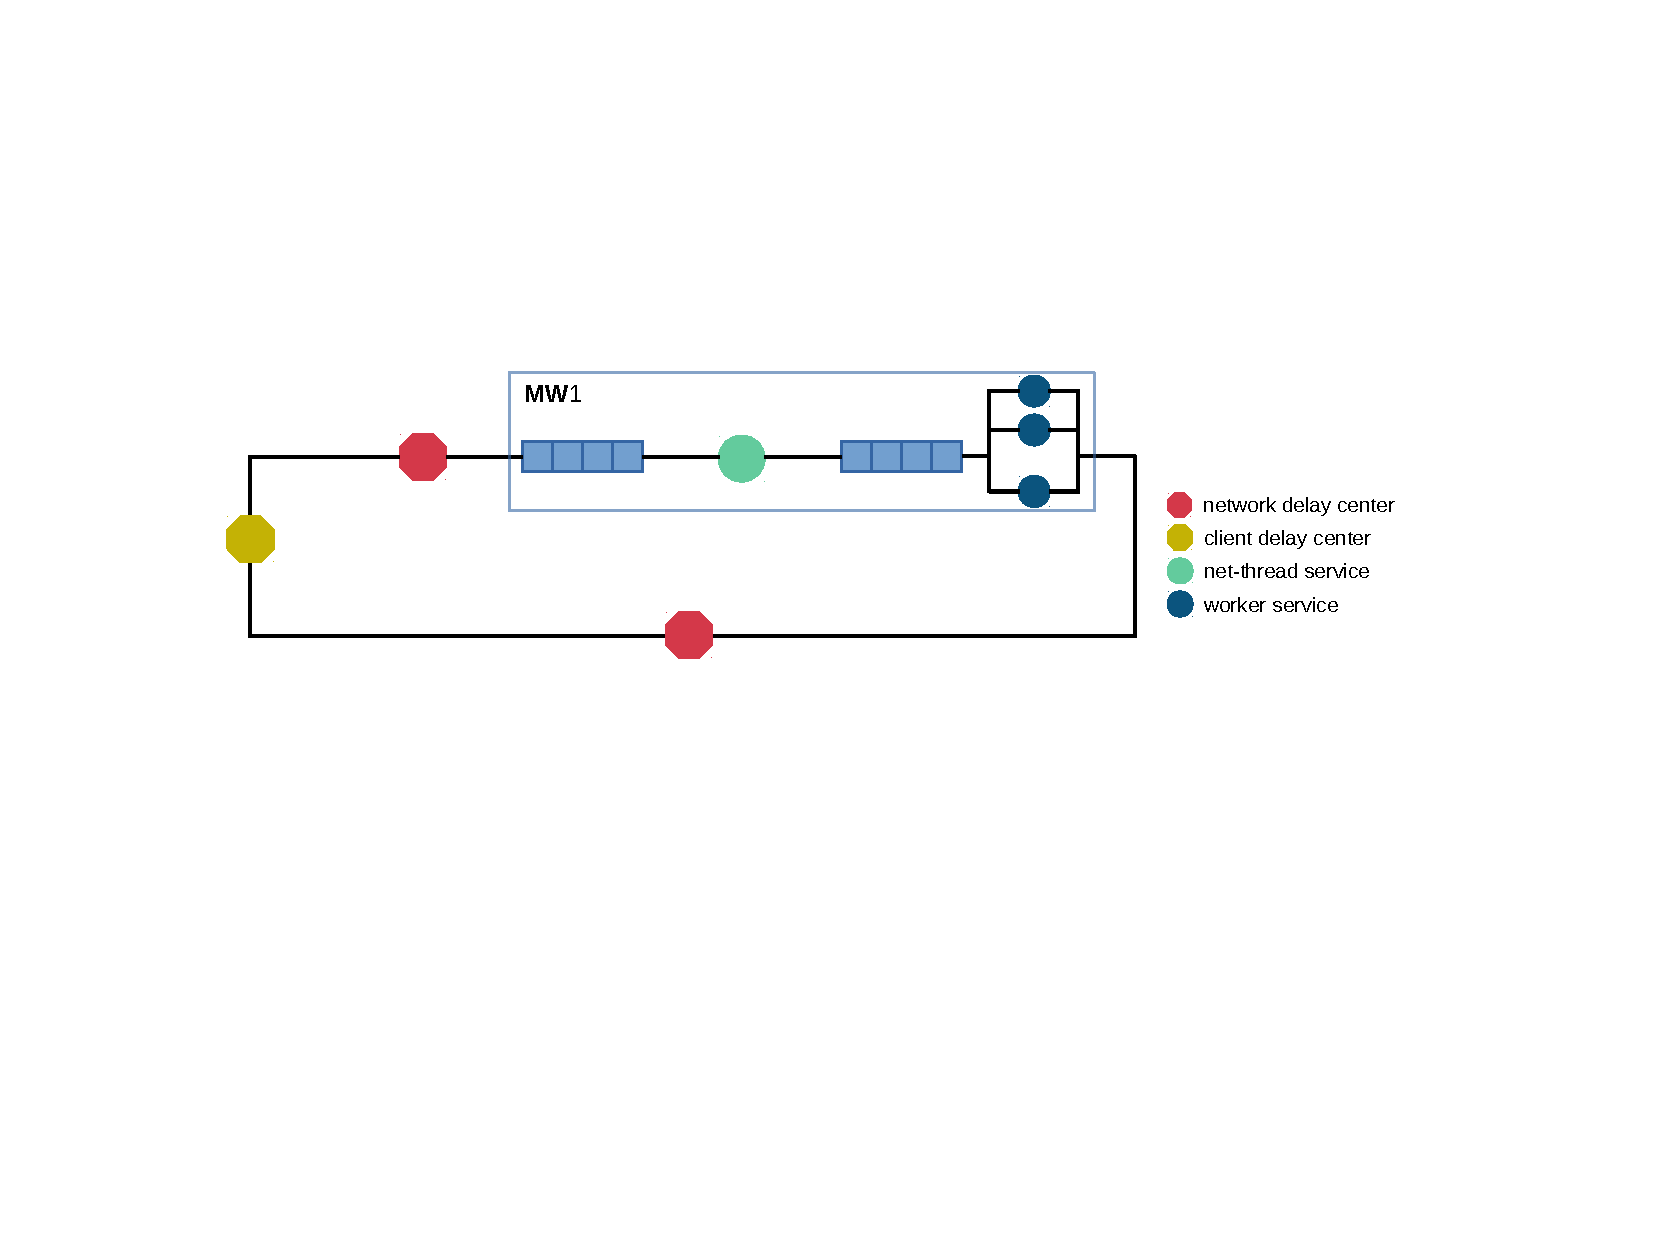
\includegraphics[width=1\linewidth]{../plots/noq_model_1midd.pdf}	
	\caption{\textit{Illustration of Network of Queues model with 1 middleware.} Net-thread is modeled as $M/M/1$ center and request queue with workers is modeled as $M/M/m$, where $m$ is number of workers.}
	\label{Figure:noq_1midd}	
\end{figure}

\textbf{\textit{Configuration with 8 workers.}} Predicted and measured results for varying read-only load (10-clients, 30-clients and 84-clients load) are displayed in table \ref{table:noq_1midd_8w}. Input to this model is: 10, 30 and 84 jobs circulating in the network, worker service time 0.89959 ms and net-thread service time is $3.830478 \cdot 10^{-3}$ ms.


\begin{table}[!ht]
	\begin{adjustbox}{center}
		\begin{tabulary}{\linewidth}{ C | C | C | C | C | C | C | }
			\cline{2-7}	&	\multicolumn{2}{| c |}{\textbf{10 clients}}	&	\multicolumn{2}{| c |}{\textbf{30 clients}}	&	\multicolumn{2}{| c |}{\textbf{84 clients}}	\\
			\cline{2-7} &	predicted	&	measured	&	predicted	&	measured	&	predicted	&	measured	\\
			\hline	\multicolumn{1}{| c |}{$R_{mw}$ [ms]}	&	0.90	&	1.03	&	2.17	&	2.6		&	5.49	&	8.49	\\
			\hline	\multicolumn{1}{| c |}{$X$ [req/s]}		&	5249	&	5106.61	&	8891.8	&	8194.38	&	9439.7	&	8299.94	\\
			\hline	\multicolumn{1}{| c |}{$Q_{mw}$}		&	4.73	&	2.02	&	19.29	&	13.29	&	51.87	&	64.43	\\
			\hline	\multicolumn{1}{| c |}{$U_{mw}$ [\%]}	&	59	&	-		&	99.98	&	-		&	\textgreater100	&	-	\\
			\hline	\multicolumn{1}{| c |}{$U_{nt}$ [\%]}	&	2	&	-		&	3.4	&	-		&	3.6	&	-	\\
			\hline 
		\end{tabulary}
	\end{adjustbox}	
	\caption{\textit{Results for Queueing Model with configuration: 1 middleware, 8 workers, read-only load}}
	\label{table:noq_1midd_8w}
\end{table}

Predicted response time and throughput under 10-client load are slightly over-optimistic, but very close to measured values. Predicted queue size is double the measured queue size, but both values are very small. Utilization of middleware is just above 50\%, implying that system is under-saturated, which can be verified in Figure \ref{Figure:baseline_1midd:a}. Net-thread is utilized around 2\%, which leaves the middleware as bottleneck. Under 30-client load, throughput is higher and response time is lower compared to corresponding measured values, but estimated values are still very good approximation of measured ones. Estimated queue size is again higher than measured one, but the difference is only 6 requests. Utilization of middleware increased to 99.98\% which clearly indicates that bottleneck is middleware. Note that for 30-clients load, system with 8 workers reaches saturation. Under 84-clients load, again, throughput is higher and response time lower than measured values, but still close to each other. Most importantly, queue size follows measured queue size, with around 19\% less requests predicted. However, numerical instabilities are observed here for the first time, expressed as middleware utilization higher than 1. Note that with this load, the system is well into saturated phase and busy all the time, and utilization should be very high.

From above mentioned, we can conclude that this network of queues models real-world system satisfactory, as all tendencies observed in experiments are visible in predictions (response time increases with load, and so does queue size for example) and predicted values are close to measured ones. However, for configuration where system is well into saturated phase, numerical instabilities were observed, hence results are not as representative.


\textbf{\textit{Configuration with 32 workers.}} Predicted and measured results for varying read-only load (10-clients, 30-clients and 84-clients load) are displayed in table \ref{table:noq_1midd_32w}. Input to this model is: 10, 30 and 84 jobs circulating in the network, worker service time 2.77046 ms and net-thread service time is $3.9558 \cdot 10^{-3}$ ms.

\begin{table}[!ht]
	\begin{adjustbox}{center}
		\begin{tabulary}{\linewidth}{ C | C | C | C | C | C | C | }
			\cline{2-7}	&	\multicolumn{2}{| c |}{\textbf{10 clients}}	&	\multicolumn{2}{| c |}{\textbf{30 clients}}	&	\multicolumn{2}{| c |}{\textbf{84 clients}}	\\
			\cline{2-7} &	predicted	&	measured	&	predicted	&	measured	&	predicted	&	measured	\\
			\hline	\multicolumn{1}{| c |}{$R$ [ms]}		&	2.77	&	0.85	&	2.77	&	1.44	&	3.04	&	5.77	\\
			\hline	\multicolumn{1}{| c |}{$X$ [req/s]}		&	3604.3	&	6050.78	&	10812	&	10330.25	&	10991	&	10565.1	\\
			\hline	\multicolumn{1}{| c |}{$Q_{mw}$}		&	9.99	&	2.76	&	29.96	&	6.51	&	33.39	&	21.66	\\
			\hline	\multicolumn{1}{| c |}{$U_{mw}$ [\%]}	&	15.6	&	-		&	93.6	&	-	&	95.2	&	-	\\
			\hline	\multicolumn{1}{| c |}{$U_{nt}$ [\%]}	&	1.42	&	-		&	4.28	&	-	&	4.35	&	-	\\
			\hline 
		\end{tabulary}
	\end{adjustbox}	
	\caption{\textit{Results for Queueing Model with configuration: 1 middleware, 32 workers, read-only load}}
	\label{table:noq_1midd_32w}
\end{table}

Predictions for 10-client load are not very accurate: estimated throughput is half the measured value, response time is 3 times higher and queue size is around 4 times higher. We can conclude that for very low utilizations (when number of jobs is significantly lower than number of workers), the model is not accurate. However, under 30-clients load, estimated throughput is very good approximation of measured value, but slightly too optimistic. Estimated response time is slightly higher than measured value, but queue size is significantly higher than measured value. Note that in this configuration, the bottleneck was server (the maximal outbound bandwidth of server physical machine, to be exact), and instead of waiting in the queue of the middleware, requests wait on server's side. As worker services in this model "absorb" the server, this high queue size values actually make sense, because they represent jobs waiting in the middleware and in the server. Similar situation for 84-clients load: throughput slightly higher, queue size higher than measured, response time lower, but close to measured value.

Generally, the model indicates that bottleneck is always the middleware, as it has the highest utilization value. However, in the experiments, middleware was bottleneck only for 8-workers configuration (which matches with findings here), but for 32-workers configuration, it was server, but since it's absorbed by middleware, findings of the model match the bottleneck identified through experiments.

It seems that higher number of workers leads to slightly worse results in predictions. This can be due to the fact that we use overly-optimistic service rates for net-thread and workers, and more workers will lead to higher deviations. On the other hand, tendencies identified in the experiments, like increase in throughput and queue size with increase in load, are visible in predictions as well, with keeping in mind that workers include processing time of the server.

\subsubsection{Network of Queues with 2 middleware}

As in baseline experiment with 2 middlewares under read-only load the bottleneck was again the server, here results for write-only load with 2 middlewares and 2 client machines are presented. Individual components remained the same: each network section is modeled as delay-center, each net-thread is modeled as $M/M/1$ and each queue with workers is modeled as $M/M/m$, only now there are 2 middlewares. Full visualization of the network is illustrated in Figure \ref{Figure:nog_2midd}. Note that half the load from client goes to each middleware.

\begin{figure}[ht!]
	\centering		
	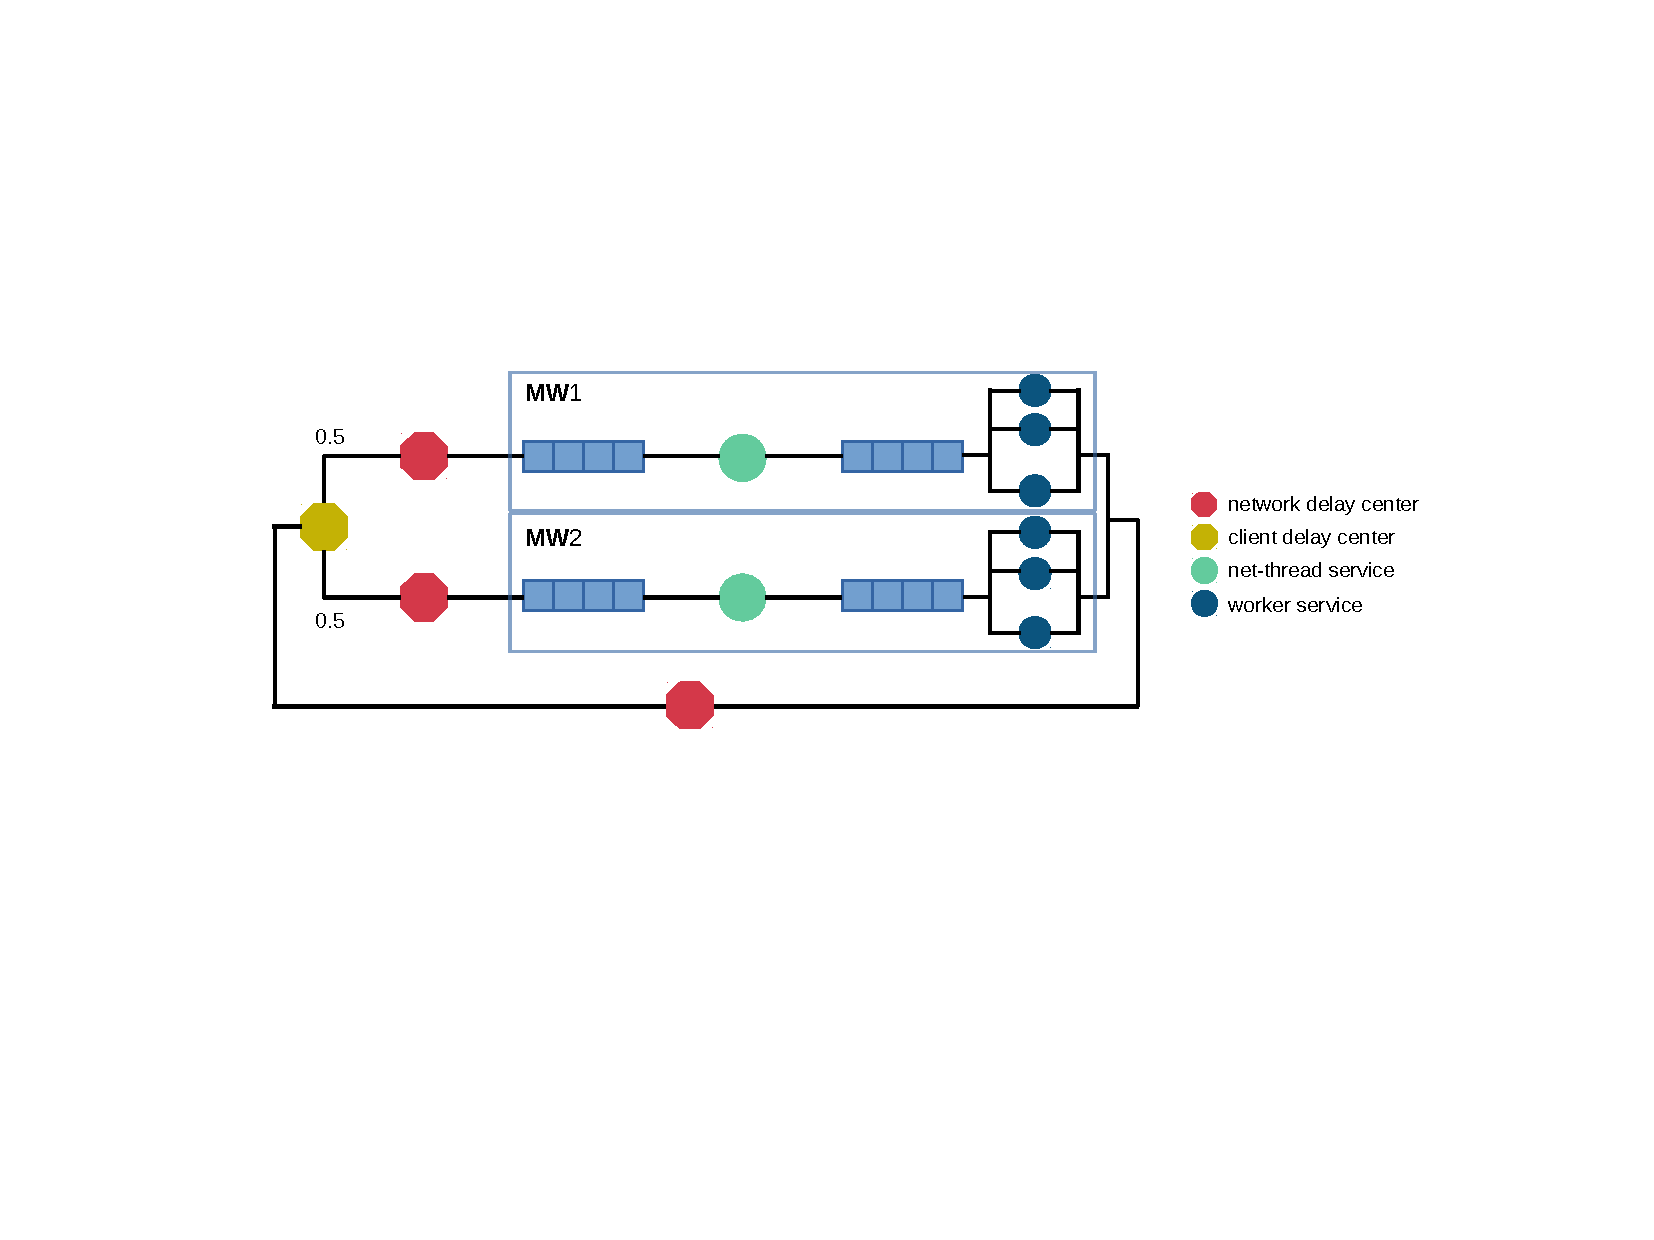
\includegraphics[width=1\linewidth]{../plots/noq_model_2midd.pdf}	
	\caption{\textit{Illustration of Network of Queues model with 2 middlewares.} Half of the load from the client (modeled as delay center) goes to each of the middlewares through network. Net-Thread is modeled as $M/M/1$ and internal request queue with workers as $M/M/m$ where $m$ is number of workers.}
	\label{Figure:nog_2midd}	
\end{figure}

With network modeled as in figure \ref{Figure:nog_2midd} and with input values obtained from experiments, numerical instabilities of MVA algorithm were observed more frequently, making it impossible to reach values that make sense for load higher than 168 clients. This instability manifests as either utilization higher than 1 on middleware(s), and/or as negative values in response time, throughput and queue size. Even though significant effort was put into tuning input parameters to find stable solution, it was impossible to do it for client-loads higher than 168 clients. Therefore, results for 60- and 168-client load are presented. Under these loads, system required little or no tuning.

\textbf{\textit{Configuration with 8 workers.}} Predicted and measured results for varying write-only load (60-clients, 168-clients) are displayed in table \ref{table:noq_2midd_8w}. Input to this model is: 60 and 168 jobs circulating in the network, worker service time 2.085 ms and net-thread service time is $1.1661 \cdot 10^{-2}$ ms.

\begin{table}[!ht]
	\begin{adjustbox}{center}
		\begin{tabulary}{\linewidth}{ C | C | C | C | C | }
			\cline{2-5}	&	\multicolumn{2}{| c |}{\textbf{60 clients}}	&	\multicolumn{2}{| c |}{\textbf{168 clients}}	\\
			\cline{2-5} &	predicted	&	measured	&	predicted	&	measured	\\
			\hline	\multicolumn{1}{| c |}{$R$ [ms]}		&	6.03	&	6.37	&	4.41	&	20.51	\\
			\hline	\multicolumn{1}{| c |}{$X$ [req/s]}		&	7461.9	&	7156.46	&	7173.6	&	7178.47	\\
			\hline	\multicolumn{1}{| c |}{$Q$}				&	22.49	&	13.87	&	15.81	&	67.69	\\
			\hline	\multicolumn{1}{| c |}{$U_{mw}$ [\%]}	&	93.5	&	-		&	97.23	&	-	\\
			\hline	\multicolumn{1}{| c |}{$U_{nt}$ [\%]}	&	4.18	&	-		&	4.35	&	-	\\
			\hline 
		\end{tabulary}
	\end{adjustbox}	
	\caption{\textit{Results for Queueing Model with configuration: 2 middlewares, 8 workers, write-only load}.}
	\label{table:noq_2midd_8w}
\end{table}

For 60-clients load, throughput and response time estimated by the model match measured values, but are slightly overly-optimistic. On the other hand, queue size approximation does not match measured value that well.The highest utilized component in the setup is middleware, and represents bottleneck, which is confirmed by findings from experiments. Utilization of net-thread is low as expected since net-thread performs very short processing (which is visible from input service time for net-thread as well). For 168-client load, throughput matches almost perfectly measured value, but the rest of the estimates do not match well. Utilization of the middleware is again the highest, and it is the bottleneck in the experiment, which again matches findings from experiments.

Finally, we have observed that for low-client load, model gives the most accurate estimates. For 8-workers configuration, the system has just reached saturation, but for 168-client load it is well into saturated phase, and the model is, unfortunately, not able to capture the behavior well with load that high, and for even higher load, the model is numerically unstable.

\textbf{\textit{Configuration with 32 workers.}} Predicted and measured results for varying write-only load (60-clients, 168-clients) are displayed in table \ref{table:noq_2midd_32w}. Input to this model is: 60 and 168 jobs circulating in the network, worker service time 2.08475 ms and net-thread service time is $1.16611 \cdot 10^{-2}$ ms. 

\begin{table}[!ht]
	\begin{adjustbox}{center}
		\begin{tabulary}{\linewidth}{ C | C | C | C | C | }
			\cline{2-5}	&	\multicolumn{2}{| c |}{\textbf{60 clients}}	&	\multicolumn{2}{| c |}{\textbf{168 clients}}	\\
			\cline{2-5} &	predicted	&	measured	&	predicted	&	measured	\\
			\hline	\multicolumn{1}{| c |}{$R$ [ms]}		&	3.68	&	2.66		&	1.23	&	6.83	\\
			\hline	\multicolumn{1}{| c |}{$X$ [req/s]}		&	11766	&	11778.92	&	15155	&	15437.57	\\
			\hline	\multicolumn{1}{| c |}{$Q$}				&	21.67	&	2.41		&	9.32	&	22.11	\\
			\hline	\multicolumn{1}{| c |}{$U_{mw}$ [\%]}	&	67.72	&	-			&	87.2	&	-	\\
			\hline	\multicolumn{1}{| c |}{$U_{nt}$ [\%]}	&	8.12	&	-			&	10.45	&	-	\\
			\hline 
		\end{tabulary}
	\end{adjustbox}	
	\caption{\textit{Results for Queueing Model with configuration: 2 middlewares, 32 workers, write-only load}}
	\label{table:noq_2midd_32w}
\end{table}

For 60-client load, estimated throughput matches almost perfectly throughput measured on the middleware and response times are similar with around 1 ms difference. Queue size, however, does not match measured value. The highest utilized component estimated by the model is middleware, indicating that middlewares are the bottleneck in the system which matches findings from experiments. Note that net-thread is utilized more with 32 workers than with 8 workers, even though the load is the same. The reason for this is faster circulation of the same number of jobs in the system that has 4 times more workers. For 168-client load (which demanded a lot of tuning) estimates match well only for throughput. The rest of estimated parameters are very different from measured values. Again, the bottleneck is middleware  since it is component with highest utilization. Utilization of net-thread is higher now, which was expected since the number of jobs circulating in the network increased.

\subsubsection{Conclusion}

The models designed are always correct when predicting the bottleneck of the system, since utilization of the middleware(s) is always the highest. Note that, in model for read-only load and 1 middleware, the bottleneck in real-world setup is server, but since it's "absorbed" by the workers, the model is still correct.

Throughput estimates often match measured values, response time estimates not so often, but are usually good. It has been observed that model estimates are more accurate under low load and low number of workers, and as either or both parameters increase, model becomes less accurate and then numerically unstable. Input values to the models are best-effort estimates of true service time of corresponding services, but these estimates are not reached by all threads in practice. It is my guess that with more workers on the same machine (same CPU), it is more difficult for individual thread to reach this service-time estimation, and this behavior cannot be captured by the model. Instead, model should show overly-optimistic estimates, which it does, especially for response time and queue size.

\end{document}
